\chapter{Cryogenic Instrumentation and Slow Controls}
\label{ch:dp-cisc}

% \fixme{Add more information about what is identical and what is different between DP and SP versions.} -- done (Glenn)

%%%%%%%%
\section{Introduction} 

The \dfirst{cisc} consortium provides comprehensive monitoring for all detector components and for liquid and gaseous argon quality and behavior as well as a control system for many detector components.
The \dword{dp} and \dword{sp} modules both use the same control
system and have nearly identical cryogenic instrumentation except
for differences in location due to the different \dword{tpc}
geometries and the presence of dedicated instrumentation for
monitoring temperature and pressure in the gas phase for the
\dword{dpmod} which is unnecessary in the \dword{spmod}.  
%The corresponding chapter of Volume~3 
\spchcisc{} of this \dword{tdr} is
virtually the same as this chapter apart from those few
differences.

The consortium responsibilities are split into 
two main branches: cryogenic instrumentation and slow controls (see Figure~\ref{fig:cisc-subsystem-chart}). 
% provides a subsystem chart for the \dword{cisc} system. 

\begin{dunefigure}[CISC subsystem chart]{fig:cisc-subsystem-chart}
  {CISC subsystem chart.}
  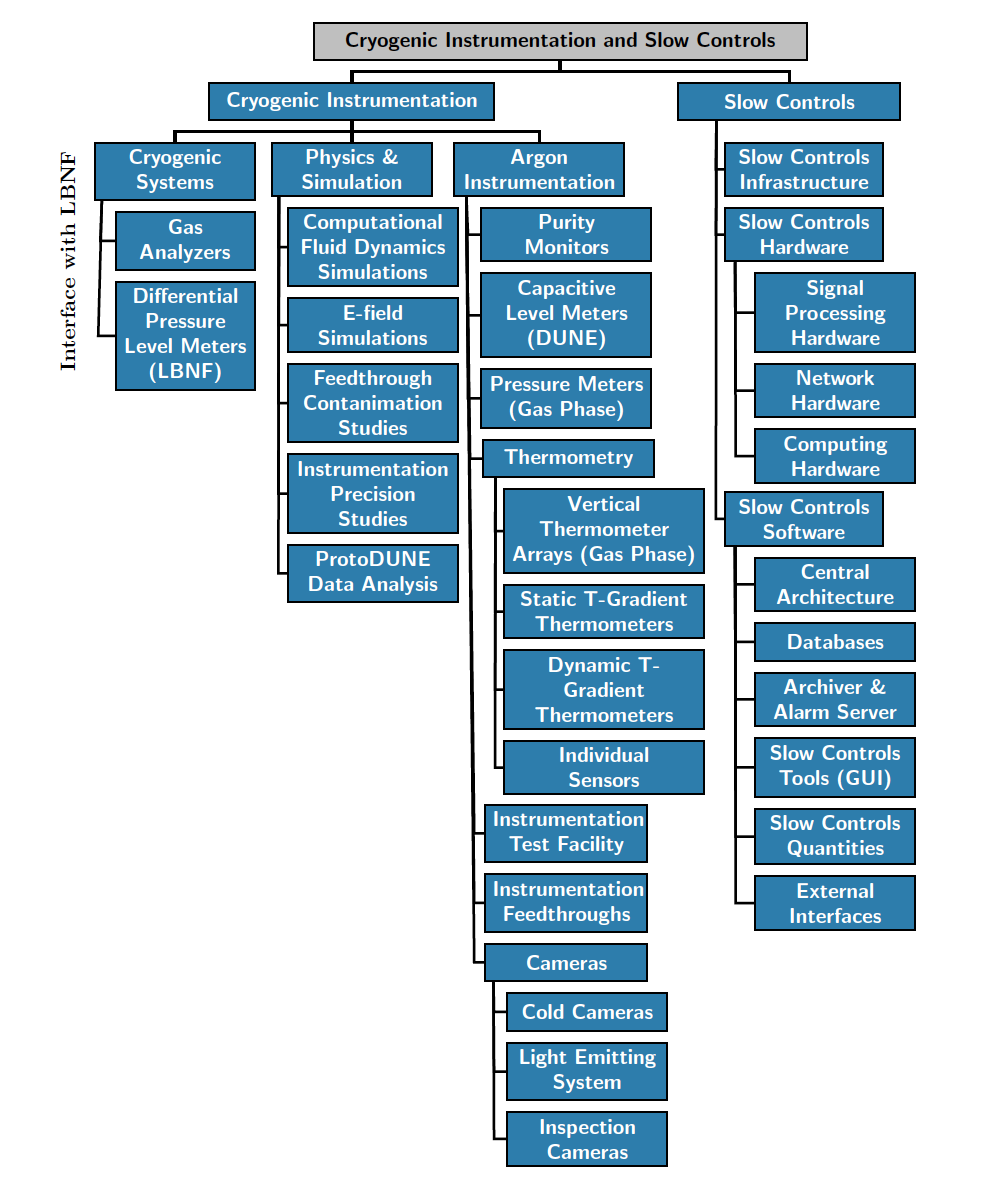
\includegraphics[width=0.8\textwidth]{graphics/CISC_scope-v2-dp-zoomed.png}
\end{dunefigure}

Each element of \dword{cisc} contributes to the DUNE physics program primarily by maintaining high detector live time.  As described in Volume~\volnumberphysics{}, \voltitlephysics{}, of this \dword{tdr}, neutrino \dword{cpv} and resolution of the neutrino mass hierarchy over the full range of possible neutrino oscillation parameters will require at least a decade of running the \dword{fd}.  Similar requirements apply to searches for nucleon decay and \dword{snb} events from within our galaxy.  Throughout this long run time, the interior of any DUNE cryostat remains completely inaccessible.  Repairs cannot be made to any damaged components within the \dword{tpc} structure; hence, environmental conditions that present risks must be detected and reported quickly and reliably. 
 
Detector damage risks peak during the initial fill of a module with \lar because temperature gradients take on their highest values during this phase.  For example, thermal contractions outside of the range of design expectations could result in broken extraction grid wires or poor connections at the cathode \dword{hv} feedthrough point that could lead to unstable \efield{}s. 
%broken \dword{apa} wires, \dwords{sipm} in \dwords{pd} that detach from the \dword{xarapu} light detectors, or 
Additional care is needed to monitor the
gas phase above the liquid level. The temperature and the pressure of the gas phase affect gas density, and consequently, the large electron multiplier (LEM) gain calibration. These considerations require a robust temperature monitoring system for the detector both in liquid and gas phase and a pressure monitoring system in the gas phase,  
%\todo{SG: list out devices for both temperature and pressure, and say liquid and gas phase} 
supplemented with liquid level monitors and a high-performance camera system for visual inspection of the interior of the cryostat during the filling process.  These systems are fully described in Section~\ref{sec:fdgen-cryo-instr} of this chapter.
 
Argon purity must be established as early as possible in the filling process, a period during which gas analyzers are most useful, and must maintain an acceptable value, corresponding to a minimum electron drift lifetime of \SI{3}{ms} %\todo{SG: the lifetime value needs to updated for DP}, 
throughout the data-taking period. Dedicated purity monitors (Section~\ref{sec:fdgen-slow-cryo-purity-mon}) provide precise lifetime measurements up to values of \SI{10}{ms} (current capability based on \dfirst{pdsp}). Purity requirements are more stringent in a dual phase detector due to longer drift paths, so \dword{cisc} plans to build longer purity monitors to increase this capability to approximately \SI{20}{ms} for the \dword{dp} \dword{fd}.
%,\todo{this will be longer for DP; contact Laura, Alan, Pordes, Jianming; modify the presentation.} the range over which electron attenuation most affects \dword{s/n} in the TPC. 
The purity monitors and gas analyzers remain important even after high lifetime has been achieved because periodic detector top-off  fills occur; the new \lar must be very high quality to be introduced into the cryostat.
 
 
The \dword{cisc} system must prevent fault conditions that could develop in the \dword{detmodule} over long periods of operation.
%\fixme{CP: specific for SP, to modify; SG: I don't know enough about DP to edit this. ACV is fixing this "[[ ]]"}
A drop in liquid level could affect the behavior of the extraction grid, which lies 5 mm below the liquid surface; the liquid level monitors must head off this possibility.  Very slow-developing outgassing phenomena could conceivably occur, with associated bubble generation creating another source of \dword{hv} breakdown events.
The cold camera system allows bubbling sites to be detected and identified, and mitigation strategies to be developed such as reducing \dword{hv} operation for some time.  A more subtle  fault is the formation of quasi-stable eddies in argon fluid flow that could prevent positive argon ions from being cleared from \dword{tpc} volume, resulting in space charge build up that would not otherwise be expected at the depth of the \dword{fd}.  The space charge could in turn cause distortions in the \dword{tpc} drift field that degrade tracking and calorimetry performance.  The high-performance thermometry  of the DUNE \dword{cisc} system creates input for well developed complex fluid flow models described in Section~\ref{sec:fdgen-cryo-cfd} that should enable detecting conditions associated with these eddies.
 
Finally, a high detector live-time fraction for operation over several years cannot be achieved without an extensive system for monitoring all aspects of detector performance, reporting this information intelligently to detector operators, and archiving the data for deeper offline studies.  Section~\ref{sec:dp-cisc-slowctrl} details the \dword{dune} slow controls system designed for this task.

%\fixme{SG: I edited the below for DP} 
Some of the baseline designs for the \dword{cisc} systems (e.g., pressure meters in gas, capacitive level meters, slow controls system) have been used in \dword{pddp}, % designs arethe baseline for all \lar instrumentation devices, and %requirements for 
and corresponding design parameters are extrapolated from these designs. For systems that are currently not deployed in \dword{pddp}, the goal is deploy them in \dword{pddp}-Run-II phase. The \dword{pddp} data from Run-I and Run-II will be used to validate the instrumentation designs and to understand their performance. For some of the \dword{cisc} systems (e.g., static and dynamic T-gradient thermometers, purity monitors), validation and performance in \dword{pdsp} will provide important inputs to \dword{dp} \dword{fd}. More details are provided in sections~\ref{sec:pddp-cfd-valid}, \ref{sec:pddp-cryo-valid}, and \ref{sec:cisc-slow-control-pdsp}.


%\subsection{Components}
\subsection{Scope}
\subsubsection{Cryogenic Instrumentation}
%The devices included under c
Cryogenic instrumentation includes purity monitors, various types of temperature monitors (gas and liquid phase), capacitive level meters, pressure meters (gas phase), and cameras with their associated light emitting systems. Also included are %components like 
gas analyzers and differential pressure level monitors that are directly related to the external cryogenics system, which have substantial interfaces with the \dword{lbnf}. \dword{lbnf} provides the needed expertise for these systems and is responsible for the design, installation, and commissioning, while the \dword{cisc} consortium provides the resources and supplements labor as needed. 

A \dword{citf} for the instrumentation devices is also part of the cryogenic instrumentation.
 \dword{cisc} is responsible for design through commissioning in the \dword{dpmod} %\dfirst{fd}.
of liquid and gaseous argon instrumentation devices: purity monitors, thermometers, capacitive level meters, pressure meters, cameras, and light-emitting system, and their associated feedthroughs.
%and the \dword{citf}.

Cryogenic instrumentation %also 
requires significant physics and
simulation work, such as \efield simulations and cryogenics modeling
studies using \dfirst{cfd}. \efield simulations
%are required to 
identify desirable locations for instrumentation
devices in the cryostat, away from %so they are not in 
regions of high \efield, so %and 
their presence does not induce large field distortions. 
% AC. What do we mean by distortions here ?
% Alternative: ``that their designs do not induce high \efields and risk of dielectric breakdown. ``
\dword{cfd} simulations help identify %are needed to understand 
expected temperature, impurity, and velocity flow distributions and guide the placement and distribution of instrumentation devices inside the cryostat.

%%%%%%%%%%%%
\subsubsection{Slow Controls}
\label{sec:dp-cisc-slowctrl}
The slow controls portion of \dword{cisc} comprises three main components: 
hardware, infrastructure, and software. The slow controls hardware and infrastructure comprises networking hardware, signal processing hardware, computing hardware, and associated rack infrastructure. The slow controls software provides, for every slow control quantity, the central slow controls processing architecture, databases, alarms, archiving, and control room displays.


%For slow controls, 
\dword{cisc} provides software and infrastructure for controlling and monitoring all detector elements that provide data on the health of the \dword{detmodule} or conditions important to the experiment, as well as  certain hardware. %Slow controls includes the systems detailed below.

%\textbf{Slow controls base software and databases:}
Slow controls base software and databases are the central tools needed to develop
control and monitoring for various detector systems and interfaces. These include:
\begin{itemize}
\item base input/output software;
\item alarms, archiving, display panels, and similar operator interface tools; and 
\item slow controls system documentation and operations guidelines.
\end{itemize}

%\textbf{Slow controls for external systems:} 
Slow controls for external systems collect data from systems
external to the \dword{detmodule} and provide status monitoring to operators
and for archiving. %These systems include 
They %will 
collect data on beam status, cryogenics status,
\dword{daq} status, facilities systems status, interlock
status bit monitoring (but not the actual interlock mechanism), ground
impedance monitoring, and possibly building and detector hall
monitoring, as needed. 

The \dword{ddss} can provide inputs to \dword{cisc} on safety interlock status, and \dword{cisc} will monitor and make that information available to the experiment operators and experts as needed. However, \dword{ddss} and \dword{cisc} are separate monitors, and the slow controls portion of \dword{cisc} does not provide any inputs to \dword{ddss}. A related question is whether \dword{cisc} can provide software intervention before a hardware safety interlock. In principle such intervention can be implemented in \dword{cisc}, presumably by (or as specified by) the hardware experts. For example, at \dword{pdsp}, the automatic lowering of \dword{hv} to clear streamers was implemented in the software for the \dword{hv} control using \dword{cisc}-level software. 

%\textbf{Slow controls for detector hardware systems:}\
Slow controls %for detector hardware systems %develop 
covers software interfaces for detector hardware devices:
\begin{itemize}
\item monitoring and control of all power supplies,
\item full rack monitoring (rack fans, thermometers and rack protection system),
\item \dword{cisc} instrumentation device monitoring (and control to the extent needed),
\item calibration device monitoring (and control to the extent needed),
\item \dword{crp} instrumentation device monitoring (and control to the extent needed),
\item power distribution unit and computer hardware monitoring,
\item \dword{hv} system monitoring through cold cameras, and
\item inspection of detector components using warm cameras.
\end{itemize}
%
%\textbf{Slow controls hardware:} 
\dword{cisc} will develop, install, and commission any hardware related to rack monitoring and control for the detector racks. Most power supplies may only require a cable from the device
to an Ethernet switch, but some power supplies might require special cables (e.g., GPIB or RS232) for communication. The \dword{cisc} consortium will provide these control cables.

%In addition to the listed activities, 
\dword{cisc} %also has 
participates in additional activities outside the scope of the consortium that require coordination with other groups. This is discussed in Section~\ref{sec:interfaces}.

%\subsection{Requirements}
\subsection{Design Considerations}
 
%Some common 
Important design considerations for instrumentation devices include stability, reliability, and longevity, so that devices can survive for at least \dunelifetime. 
Such longevity is uncommon for any device, so the overall design allows replacement of devices where possible.
Some devices are critical for filling and commissioning but less critical for later operations; for these devices we specify a minimum lifetime of 18 months and 20 years as a desirable goal.
\dword{dune} requires the \efield on any instrumentation devices inside the cryostat to be less than \localefield to minimize the risk of dielectric breakdown in \lar. 

An important consideration for event reconstruction is the maximum noise level, induced by instrumentation devices, that the readout electronics  can tolerate. \dword{pddp} is evaluating this. Table~\ref{tab:specs:DP-CISC} shows the selected top-level specifications for \dword{cisc} subsystems. 
%\todo{SG: Table 1.1 needs to be updated with DP-specific requirements if any. ACV/SG following up.} 
Tables~\ref{tab:fdgen-slow-cryo-requirements-1}, \ref{tab:fdgen-slow-cryo-requirements-2}, and \ref{tab:fdgen-slow-cryo-requirements-3} show the full set of specifications
for the \dword{cisc} subsystems. In all those tables two values are quoted for most of the design parameters: 1) specification, which is the minimal requirement to guarantee the detector performance, and 2) goal,  an improved version enabling more detailed studies which could lead to an improved design of the cryogenics system for subsequent detectors. 
% Won't fix, it's ok. \fixme{"3rd draft" or supplement : In table 1.1 and 1.2, need to update the precision on PrM and present it differently e.g. relative vs absolute}

Data from purity monitors and different types of thermometers will be used to validate the \lar fluid flow model. 
A number of requirements drive the design parameters for the precision and granularity of monitor distribution across the cryostat. 
For example, the electron lifetime measurement precision must be \SI{2.3}{\%} to keep the bias on the charge readout in the \dword{tpc} below \SI{0.5}{\%} at \SI{5}{ms} lifetime.
 For thermometers, the 
parameters are driven by \dword{pdsp} and  \dword{pddp} designs as well as the comparison of \dword{pdsp} data to \dword{cfd} simulations. The temperature measurement resolution in the liquid phase must be less than \SI{2}{mK}, and the relative precision of those measurements must be less than \SI{5}{mK}. The resolution is defined as the temperature \dword{rms} for individual measurements and is driven by the electronics. The relative precision also includes the effect of reproducibility for successive immersions in \dword{lar}. 
The relative precision is particularly important in characterizing %because 
gradients less than \SI{20}{mK}. % should be characterized.  
As described below, the laboratory calibration data and the recent analysis of thermometer instrumentation data from \dword{pdsp} shows that a \SI{2.5}{mK} relative precision is achievable. 


It is also important to monitor the temperature and pressure in the gas phase over the liquid phase because they affect the \dword{lem} gain calibration. The gas pressure must be monitored to 1~mbar precision and accuracy. Near the surface of the liquid, the temperature gradient of the gas must be measured with an array of temperature probes with a vertical pitch that increases with height (from 1 to 5 cm). The \dword{lar} differential pressure level meters must be precise to \SI{14}{mm} to measure accurately during filling. 
%This precision is also sufficient to ensure that the \dword{lar} level stays above the \dwords{gp} of a \dfirst{sp} module.
Moreover, multiple capacitive level meters with better than 5~mm precision will be needed to more precisely measure the \lar level and for \lar-level based interlocks for other systems (e.g., \dword{hv}).  
%along the top of the fluid to maintain correct depth of the gas phase\todo{SG to fix this.}. 

As shown in Table~\ref{tab:fdgen-slow-cryo-requirements-2}, several requirements drive the design of cold and warm cameras and the associated light emitting system. The components of the camera systems must not contaminate the \lar or produce bubbles % when the \dword{hv} 
to avoid  increasing the risk of \dword{hv} discharge. Both cold and warm cameras must provide coverage of at least \SI{80}{\%} of the \dword{tpc} volume 
with a resolution of \SI{1}{cm} for cold cameras and \SI{2}{mm} for warm cameras on the \dword{tpc}.
% CEL: my 'fix me' with details, removed. Wanted to hold 
% if needed later in the document. 

For the \dword{citf}, a cryostat with a capacity of only \num{0.5} to approximately \SI{3}{m^3} %cubic meter is reasonable because 
will suffice and will keep turn around times and filling costs %are 
low. % for smaller cryostats. 
For gas analyzers, the operating range must allow us to establish useful electron lifetimes;
% is an important requirement; 
details  are in Table~\ref{tab:fdgen-slow-cryo-requirements-1}.

For slow controls, the system must
be sufficiently robust to monitor 
a minimum of 150,000 variables per \dword{detmodule}, and 
support a broad range of monitoring and archiving rates;
the estimated variable count, data rate, and archive storage needs
are discussed in section \ref{sec:fdgen-slow-cryo-quant}.
The system must also
interface with a large number of detector subsystems and
establish two-way communication with them for control and monitoring. 
For the alarm rate, 150 alarms/day is used as the specification as it is the maximum to which humans can be expected to respond. The goal for the alarm rate is less than 50 alarms/day. The alarm logic system will need to include features for managing ``alarm storms'' using alarm group acknowledgment, summaries, delays, and other aids.


% input of generated DP-CISC table here
% This file is generated, any edits may be lost.
\begin{footnotesize}
%\begin{longtable}{p{0.14\textwidth}p{0.13\textwidth}p{0.18\textwidth}p{0.22\textwidth}p{0.20\textwidth}}
\begin{longtable}{p{0.12\textwidth}p{0.18\textwidth}p{0.17\textwidth}p{0.25\textwidth}p{0.16\textwidth}}
\caption{Specifications for DP-CISC \fixmehl{ref \texttt{tab:spec:DP-CISC}}} \\
  \rowcolor{dunesky}
       Label & Description  & Specification \newline (Goal) & Rationale & Validation \\  \colhline

   \newtag{DP-FD-1}{ spec:dp-min-drift-field }  & Minimum drift field  &  $>$\,\SI{250}{V/cm} \newline ( $>\,\SI{500}{V/cm}$ ) &  Lessens impacts of $e^-$-Ar recombination, $e^-$ lifetime, $e^-$ diffusion and space charge. &  ProtoDUNE \\ \colhline
    
   \newtag{DP-FD-5}{ spec:lar-purity }  & Liquid argon purity  &  $<$\,\SI{100}{ppt} \newline ($<\,\SI{30}{ppt}$) &  Provides $>$5:1 S/N on induction planes for  pattern recognition and two-track separation. &  Purity monitors and cosmic ray tracks \\ \colhline
    
   
  \newtag{DP-FD-15}{ spec:dp-lar-n-contamination }  & LAr nitrogen contamination  &  $<\,\SI{25}{ppm}$ &  Maintain \SI{0.5}{PE/MeV} PDS sensitivity required for triggering proton decay near cathode. &   \\ \colhline
    
   
  \newtag{DP-FD-16}{ spec:dp-det-dead-time }  & Detector dead time  &  $<\,\SI{0.5}{\%}$ &  Meet physics goals in timely fashion. &  ProtoDUNE \\ \colhline
    
   
  \newtag{DP-FD-18}{ spec:dp-cryo-monitor-devices }  & Cryogenic monitoring devices  &   &  Constrain uncertainties on detection efficiency, fiducial volume. &  ProtoDUNE \\ \colhline
    
   
  \newtag{DP-FD-24}{ spec:dp-local-e-fields }  & Local electric fields  &  $<\,\SI{30}{kV/cm}$ &  Maximize live time; maintain high S/N. &  ProtoDUNE \\ \colhline
    
   
  \newtag{DP-FD-25}{ spec:de-non-fe-noise }  & Non-FE noise contributions  &  $<<\,\SI{1000}\,e^- $ &  High S/N for high reconstruction efficiency. &  Engineering calculation and ProtoDUNE \\ \colhline
    

   
  \newtag{DP-CISC-1}{ spec:inst-noise }  & Noise from Instrumentation devices  &  $\ll\,\SI{1000}\,e^- $ &  Max noise for 5:1 S/N for a MIP passing near cathode; per SBND and DUNE CE &  ProtoDUNE \\ \colhline
    
   \newtag{DP-CISC-2}{ spec:inst-efield }  & Max. E field near instrumentation devices  &  $<\,\SI{30}{kV/cm}$ \newline ( $<\,\SI{15}{kV/cm}$ ) &  Significantly lower than max field of 30 kV/cm per DUNE HV  &  3D electrostatic simulation \\ \colhline
    
   \newtag{DP-CISC-3}{ spec:elec-lifetime-prec }  & Precision in electron lifetime  &  $<\,$1.4\% \newline ( $<\,$1\% ) &  Required for accurate charge reconstruction per DUNE-FD Task Force report. &  ProtoDUNE and CITF \\ \colhline
    
   \newtag{DP-CISC-4}{ spec:elec-lifetime-range }  & Range in electron lifetime  &  \SIrange{0}{10}{ms} (\SIrange{0}{30}{ms}) \newline (\SIrange{0}{10}{ms} (\SIrange{0}{30}{ms})) &  Slightly more than best values so far observed in other detectors. &  ProtoDUNE and CITF \\ \colhline
    
   \newtag{DP-CISC-11}{ spec:temp-repro }  & Precision: temperature reproducibility  &  $<\,\SI{5}{mK}$ \newline (\SI{2}{mK}) &  Allows validating CFD models that predict gradients less than 15 mK. &  ProtoDUNE and CITF \\ \colhline
    
   \newtag{DP-CISC-14}{ spec:temp-stability }  & Temperature stability  &  $<\,\SI{2}{mK}$ at all places and times \newline ( Match precision requirement at all places, at all times ) &  Measures temperature map with sufficient precision for the duration of thermometer operations. &  ProtoDUNE \\ \colhline
    
   \newtag{DP-CISC-27}{ spec:camera-cold-coverage }  & Cold camera coverage  &  $>\,$80\% of HV surfaces \newline ( \num{100}\% ) &  Enables detailed inspection of issues near HV surfaces. &  Calculated from location, validated in prototypes. \\ \colhline
    
   \newtag{DP-CISC-51}{ spec:slowcontrol-alarm-rate }  & Slow control alarm rate  &  $<\,$150/day \newline ($<\,$50/day) &  Keeps rate low enough to allow response to every alarm. &  Detector module; depends on experimental conditions \\ \colhline
    
   \newtag{DP-CISC-52}{ spec:slowcontrol-num-vars }  & Total No. of variables  &  $>\,\num{150000}$ \newline (\SIrange{150000}{200000}{}) &  Scaled from ProtoDUNE &  ProtoDUNE and CITF \\ \colhline
    
   \newtag{DP-CISC-54}{ spec:slowcontrol-archive-rate }  & Archiving rate  &  \SI{0.02}{Hz} \newline ( Broad range \SI{1}{Hz} to \num{1} per few min. ) &  Archiving rate differs by variable, optimized to store important information &  ProtoDUNE \\ \colhline
    


\label{tab:specs:DP-CISC}
\end{longtable}
\end{footnotesize}


\begin{dunetable}
[Specifications for CISC subsystems (1)]
{p{0.45\linewidth}p{0.25\linewidth}p{0.25\linewidth}}
{tab:fdgen-slow-cryo-requirements-1}
{List of specifications for the different CISC subsystems (1).}   
Quantity/Parameter				                             & Specification			                                        & Goal		                                              \\ \toprowrule                     
Noise from instrumentation devices				             & $\ll$ \elecnoisefe                                      & 
\\ \colhline                     
Max. \efield near instrumentation devices				     & <\localefield			                                                & <15 kV/cm		                                          \\ \colhline                     
\textbf{Thermometers (LAr)}	                                             &                                                                      &                                                         \\ \colhline                      
Vertical density of sensors for T-gradient monitors			 & > 2 sensor/m			                                             & > 4 sensors/m		                                      \\ \colhline  
2D horizontal density for bottom individual sensors		 &  1 sensor/5(10) m 			                                        &  1 sensor/3(5) m 		                                  \\ \colhline                     
Resolution of temperature measurements				         & < 2 mK			                                                    & <0.5 mK		                                          \\ \colhline                         
Precision: temperature reproducibility 				         & < 5 mK			                                                    & 2 mK		                                              \\ \colhline                     
Stability 	  &  < \SI{2}{mK} at all places and times	 &   Match precision requirement at all places/times \\ \colhline                 
Discrepancy between laboratory and  in situ calibrations for temperature sensors			             & < 5 mK			                                                    & < 3 mK		                                          \\ \colhline                           
Discrepancy between measured temperature map and CFD simulations in \dword{pdsp}	 & < 5 mK & %< 5 mK		     
\\ \colhline                             
\textbf{Thermometers (GAr)}	                 &                              &   \\ \colhline
Thermometer density (decreases with height) &          1 sensor/2-10 cm     &    1 sensor/1-5 cm       \\ \colhline
Thermometer coverage                        &         40 cm                 &    60 cm                 \\ \colhline
Resolution of temperature measurements      &         5 mK		            &   	0.5 mK                   \\ \colhline 
Precision: temperature reproducibility 		&         100 mK			    &       100 mK	                   \\ \colhline          
\textbf{Thermometers (All)}	                 &                              &   \\ \colhline
Reliability				                         & 80\% (in 18 months)		 & 50\% (during 20 years)\\ \colhline                     
Longevity				                         & > 18 months		         & > 20 years	         \\ \colhline
\textbf{Level Meters}	          &    &          \\ \colhline            
Precision (LBNF side)		   & 0.1\% over 14 m (14 mm)			                                    & %0.1\% over 14 m (14 mm)
\\ \colhline           
Precision (capacitive level meters, \dword{dune} side) & 1~cm & <5~mm   
\\ \colhline         
Longevity		  & 20 years	   & > 20 years		                                                  \\ \colhline     
\textbf{Gas Analyzers}	   &   &  \\ \colhline            
Operating Range O2	 & 0.2 (air) to 0.1 ppt  & %Air (0.2) to 0.1 ppt
\\ \colhline    
Operating Range H2O				                             & %Nominally Air to sub ppb levels, depending on species of contaminant	
Nom. air to sub ppb; contaminant-dependent & %Air to sub ppb.  levels, depending on species of contaminant	          
\\ \colhline           
Operating Range N2				                             & Nominally Air Nom. air to sub ppb; contaminant-dependent	& %Air to sub ppm.
\\ \colhline             
Precision: 1 sigma at zero				                     & %depends on the range of the gas analyzer
per gas analyzer range
& %depends on the range of the gas analyzer		                     
\\ \colhline     
Detection limit: 3 sigma & Different analyzer modules needed to cover entire range	& %Different Gas analyzer modules are needed to cover the entire range 
\\ \colhline           
Stability   & <\% of full scale range.		 & %<\% of full scale range.
\\ \colhline         
Longevity		 & >10 years	  & %10 years  
\\
\end{dunetable}


\begin{dunetable}
[Specifications for CISC subsystems (2)]
{p{0.45\linewidth}p{0.25\linewidth}p{0.25\linewidth}}
{tab:fdgen-slow-cryo-requirements-2}
{List of specifications for the different CISC subsystems (2).}   
Quantity/Parameter		     & Specification	  & Goal   \\ \toprowrule   
\textbf{Purity Monitors}	                                             &                                                                      &                                                         \\ \colhline                      
Precision in electron lifetime				                 & <2.3\% at 5~ms (<4\% at 9~ms)			                                            & < 1\%		                                              \\ \colhline                     
Range in electron lifetime				                     & 0.04 - 10 ms  			                    & (0.04 - 30 ms inline)       
\\ \colhline                         
Longevity				                                     & \dunelifetime			                                                    & > \dunelifetime		                                      \\ \colhline                     
Stability				                                     & Match precision requirement at all places/times			    & %Match precision requirement at all places/times  
\\ \colhline  	                   
Reliability				                                     & Daily measurements			                                        & Measurements %capable of being 
as needed	  \\ \colhline 
\textbf{Pressure Meters (GAr)}	          &    &          \\ \colhline            
Relative precision (DUNE side)		   & 0.1~mbar	& %0.1\% over 14 m (14 mm)
\\ \colhline  
Absolute precision (DUNE side)		   & <5~mbar	& %0.1\% over 14 m (14 mm)
\\ \colhline  
\textbf{Cold cameras}	                                             &                                                                      &                                                                     \\ \colhline        
Coverage				                                     & 80\% of the exterior of HV surfaces			                        & 100\% 	                                                          \\ \colhline         
Frames per second	   & yet to be defined	  & %yet to be defined
\\ \colhline             
Resolution 	 & 1 cm on the \dword{tpc}	 & yet to be defined
\\ \colhline           
Duty cycle	  & yet to be defined	 & %yet to be defined
\\ \colhline         
Longevity			 & > 18 months			                                                & > 20 years		                                                  \\ 
\textbf{Inspection cameras}	     &                                                                      &                                                                     \\ \colhline        
Coverage	 & 80\% of the \dword{tpc}		  & yet to be defined		                                              \\ \colhline         
Frames per second		   & yet to be defined	   & %yet to be defined	
\\ \colhline             
Resolution 	  & 2 mm on the \dword{tpc}			                                            & yet to be defined		                                              \\ \colhline           
Heat transfer	  & no generation of bubbles			                                & 	%no generation of bubbles	
\\ \colhline         
Longevity			  & > 18 months			                                                & > 20 years		                                                  \\ \colhline         
\textbf{Light emitting system}	                                     &                                                                      &                                                                     \\ \colhline        
Radiant flux     & > 10 mW/sr		 & 100 mW/sr \\ \colhline         
Power				     & < 125 mW/LED			                                        & %\dword{alara}	
\\ \colhline           
Wavelength	   & red/green		 & IR/white	   \\ \colhline         
Longevity	  & > 18 months (for cold cameras) 			                            & > 20 years		                                              \\ \colhline         
\textbf{\dfirst{citf}}	                 &                                                                      &                                                                     \\ \colhline            
Dimensions		  & 0.5 to 3  cubic meters 			                                    & %0.5-3 cubic meters
\\ \colhline             
Temperature stability	 & $\pm$1K	 & %+- 1K
\\ \colhline                                       
Turn-Around time	 & $\sim\,$9 days   & 9 days 	  \\ \colhline                                       
LAr purity		   & O2, H2O: low enough  to measure drifting electrons of devices under test, $\sim\,\SI{0.5}{ms}$.    N2: ppm for scintillation light tests. 	        &  >1.0 ms                          
                         \\          
\end{dunetable}  

\begin{dunetable}
[Specifications for CISC subsystems (3)]
{p{0.45\linewidth}p{0.25\linewidth}p{0.25\linewidth}}
{tab:fdgen-slow-cryo-requirements-3}
{List of specifications for the different CISC subsystems (3).}   
Quantity/Parameter		     & Specification	  & Goal   \\ \toprowrule   
\textbf{Slow Controls}		                                         &                                                                      &                                                                     \\ \colhline
Alarm rate	  & <150/day			                                                    &  < 50/day                                                           \\ \colhline
Total No. of variables				                         & 150,000			                                                    &  150,000 - 200,000                                                   \\ \colhline
Server rack space				                             & 2 racks			                                                    &  3 racks                                                            \\ \colhline
Archiving rate 				                                 & 0.02 Hz			                                                    &  Broad range 1 Hz  to 1 per few min.                                \\ \colhline
Near detector status & Beam conditions and detector status	                                &  Full beam and detector status                                      \\          
\end{dunetable}  

%%%%%%%%
\subsection{Fluid Dynamics Simulation}
\label{sec:fdgen-cryo-cfd}

%\fixme{SG/ACV:DONE}

Proper placement of purity monitors, thermometers, and liquid level monitors within the \dword{detmodule} requires knowing how \lar flows within the cryostat, given its fluid dynamics, heat and mass transfer, and distribution of impurity concentrations. Fluid flow is also important in understanding how the positive and negative ion excess created by various sources (e.g., ionization from cosmic rays and $^{36}$Ar; ion feedback at the liquid-gas interface in a \dword{dp} detector) is distributed across the detector as it affects \efield uniformity. 
Finally, \dword{cfd} simulations are crucial to predict the purity of the argon in regions where experimental data is unavailable. The overall goal of the \dword{cfd} simulations
%\dword{dune} \dword{fd} 
%for the \dword{spmod} 
is to better understand and predict the fluid (in either liquid or vapor state) motions and the implications for detector performance. % of the detectors. 

Fluid motion within the cryostat is driven primarily by small changes in density caused by thermal gradients within the fluid although pump flow rates and inlet and outlet locations also contribute. Heat sources include exterior heat from the surroundings, interior heat from electronics, and heat flow through the pump inlet. In principle, purity monitors can be placed throughout the cryostat to determine if the argon is pure enough for experimentation. However, some areas inside the cryostat are off limits for such monitors. 
% \fixme{anne moved prev pgraph up --- looks good [Glenn, Carmen, Sowjanya]}


The fluid flow behavior can be determined by simulating \dword{lar} flow within a \dword{detmodule} %the detector 
using Siemens Star-CCM$+$\footnote{https://mdx.plm.automation.siemens.com/star-ccm-plus}, a commercially available \dword{cfd} code.  Such a model must properly define the fluid characteristics, solid bodies, and fluid-solid interfaces, as well as provide a way to measure contamination, while still maintaining reasonable computation times. In addition, these fluid dynamics simulations can be compared to available experimental data to assess simulation accuracy and credibility. 

%\fixme{seems like the above is sp/dp independent but the next stuff isn't. anne. The text has been modified [Carmen and Glenn] --- we think this is fixed.}
Although simulation of the \dword{detmodule} presents challenges, %there are 
acceptable simplifications can %to 
accurately represent the fluid, the interfacing solid bodies, and variations of contaminant concentrations. Because of the magnitude of thermal variation within the cryostat, modeling the \lar is simplified by using constant thermophysical properties, calculating buoyant force with the Boussinesq Model (using a constant density for the fluid with application of a temperature-dependent buoyant force), and a standard shear stress transport turbulence model. Solid bodies that touch the \lar include the cryostat wall, photon detectors, and light reflector foils.  
The \dword{fc} planes, cathode planes, and grounding grid can be represented by porous bodies. Because impurity concentration and electron lifetime do not affect fluid flow, these variables can be simulated as passive scalars, as is commonly done for smoke released \cite{cfd-1} 
in air or dyes released in liquids.


Discrepancies between real data and simulations may affect detector performance. % because 
Simulation results contribute to decisions about where to place sensors and monitors, and to %as well as 
the definitions of various calibration quantities. Methods of mitigating such risks include well established convergence criteria, sensitivity studies, and comparison to results of previous \dword{cfd} simulation work. Moreover, the simulation will be improved with input from \lar temperature and purity measurements and validation tests from \dword{pdsp}\footnote{Because \dword{pddp} was not instrumented with high-precision thermometers in the liquid phase and because the cryogenics design is the same for \dword{sp} and \dword{dp} modules of the \dword{dune} \dword{fd}, \dword{pdsp} data will be used to validate the liquid \dword{cfd} model.}. 

Taking into account that the \dword{cfd} model can predict both temperature and impurity levels, the procedure for validating and tuning the \dword{cfd} model will be the following: 1) temperature predictions will be constrained with temperature measurements in numerous locations in the cryostat to improve the \dword{cfd} model, 2) the improved model is then used to predict the \lar impurity level at the location of purity monitors, 3) this prediction is compared with the actual measurement from purity monitors to further constraint the \dword{cfd} model.  



Figure~\ref{fig:cfd-example} shows an example of the temperature
distribution on a plane intersecting an \lar inlet and at a
plane halfway between an inlet and an outlet in the \dword{spmod}.
Note the plume of higher temperature \lar between the walls and
the outer \dword{apa} on the inlet plane. The current placement of instrumentation in
the cryostat as shown in Figure~\ref{fig:cisc-dp-tsensor-map} was determined using temperature and impurity distributions from \dword{cfd} simulations.

\begin{dunefigure}[\dshort{cfd} example]{fig:cfd-example}
  {Distribution of temperature on a plane intersecting an inlet (left) and halfway between an inlet and an outlet (right), as predicted by previous \dword{cfd} simulations for the \dword{spmod} (from~\cite{bib:docdb5915}).}
  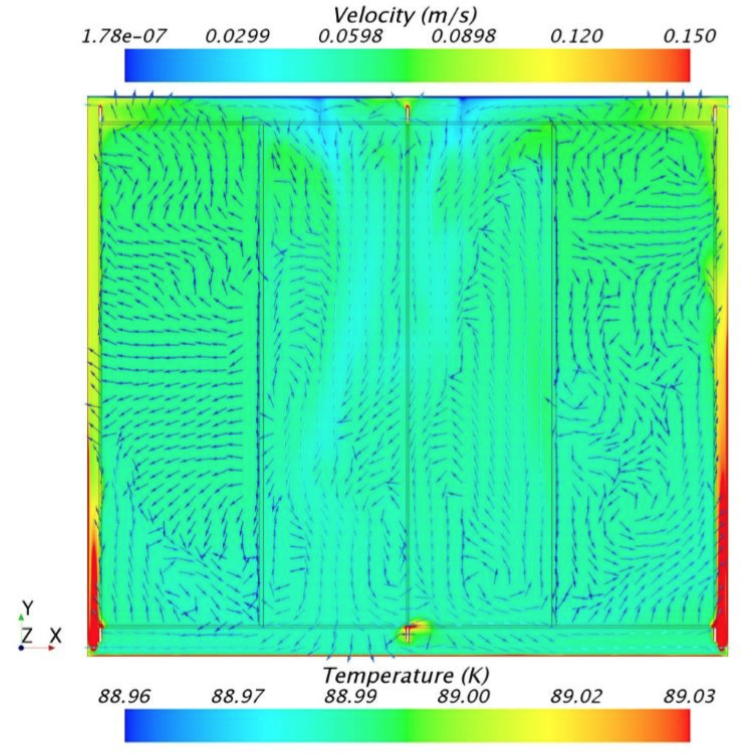
\includegraphics[height=0.4\textwidth]{cisc_cfd_inlet_z52.png}
  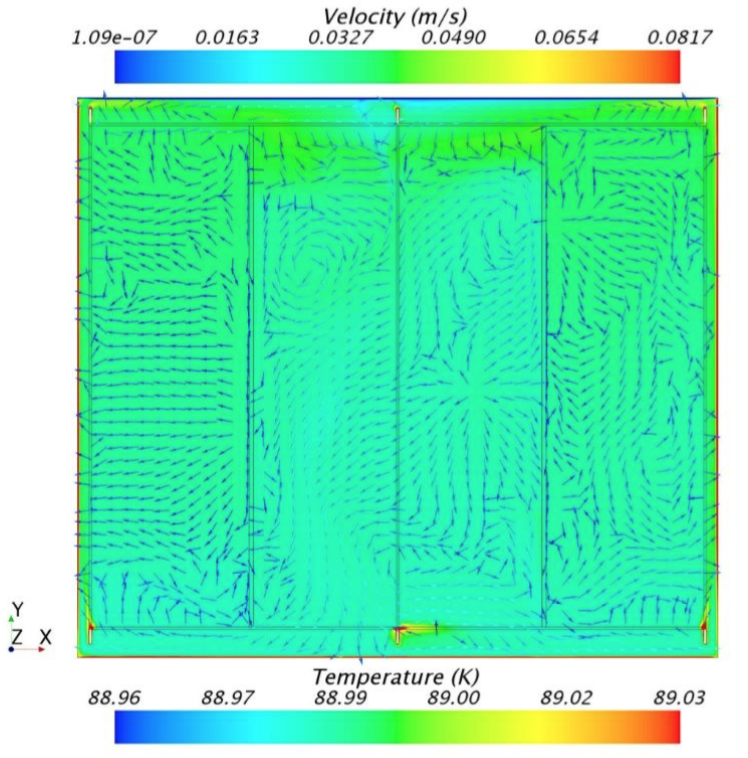
\includegraphics[height=0.4\textwidth]{cisc_cfd_outlet_z0.png}
\end{dunefigure}

\begin{dunefigure}[Distribution of temperature sensors inside the cryostat]{fig:cisc-dp-tsensor-map}
  {Distribution of temperature sensors inside the cryostat.}
  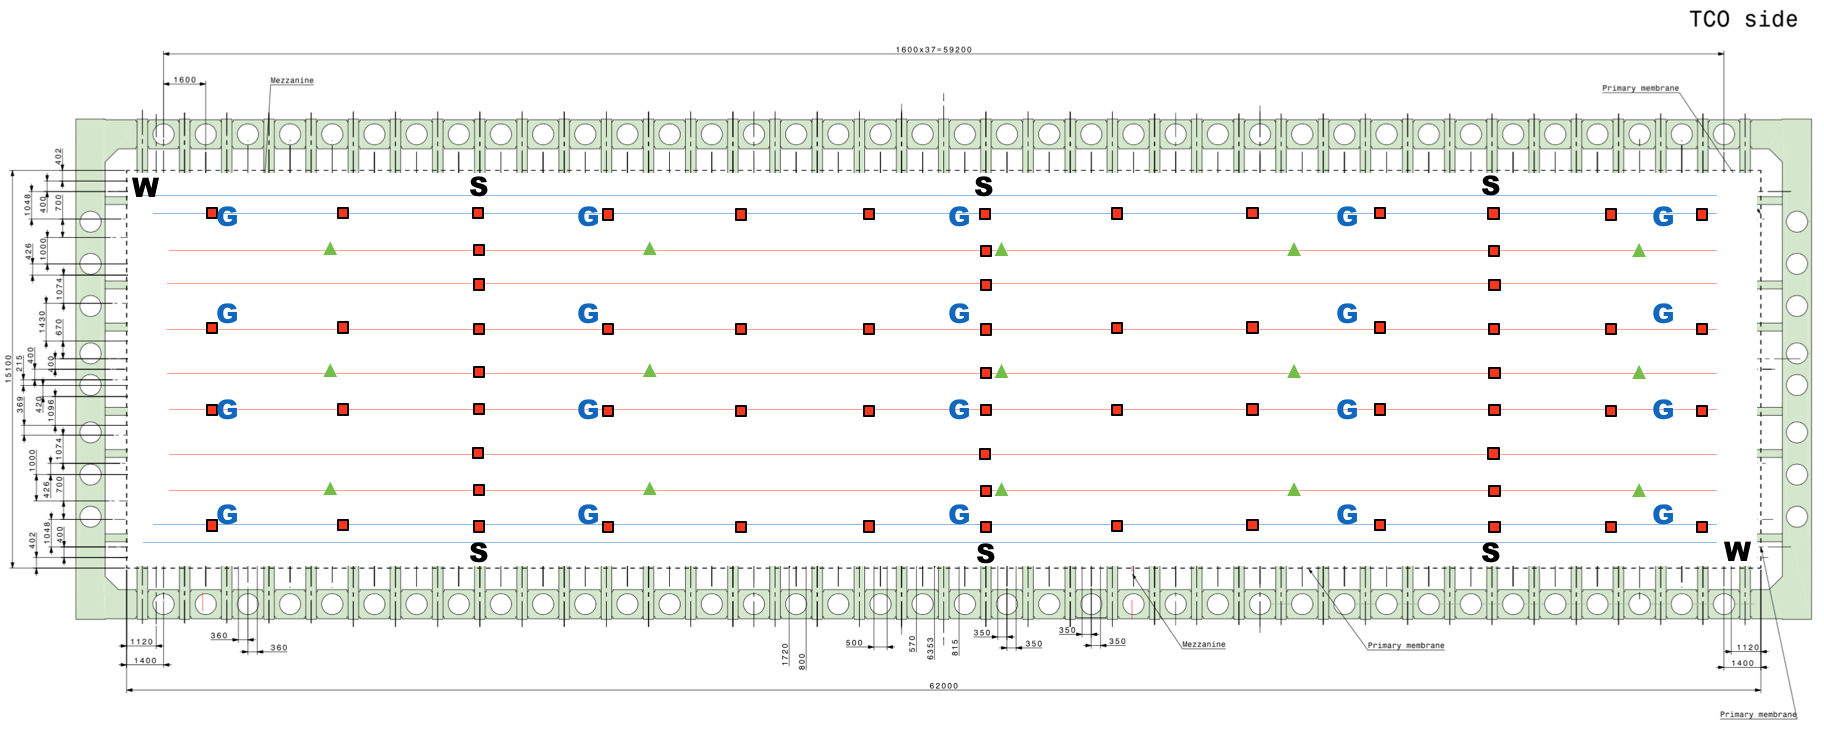
\includegraphics[width=0.95\textwidth]{cisc_dp_tsensor_map_crop.png}
  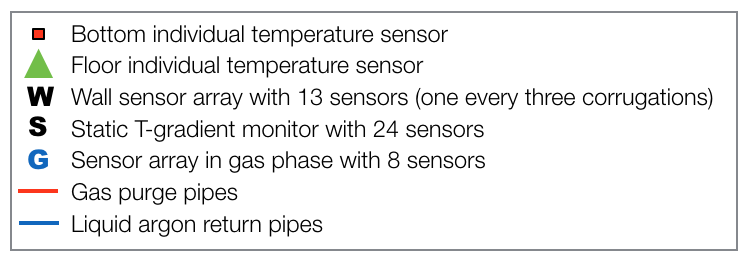
\includegraphics[width=0.50\textwidth]{cisc_dp_tsensor_map_legend.png}
\end{dunefigure}


The strategy for future \dword{cfd} simulations begins with
validating a \dword{cfd} model for \dword{pddp} using \dword{pddp} \lar instrumentation data, followed by modeling the \dword{fd} \dword{dpmod} to derive specifications for instrumentation.  See Table~\ref{tab:fdgen-cisc-CFDparam}.
We are pursuing a prioritized set of studies to help determine requirements for other systems. We plan to 
\begin{itemize}
\item review the \dword{dune} \dword{dp} \dword{fd} cryogenics system design and verify the current implementation in simulation %to ensure that the model represents what will be built.
to ensure that the simulation represents the actual design;
\item validate the liquid \dword{cfd} model using thermometer data from \dword{pdsp} because we have no high precision T-gradient thermometers in \dword{pddp} to validate the liquid model; 
\item model the \dword{pddp} gas regions with the same precision as the \dword{fd}. The gas model should how to place thermometers in the argon gas and verify the design of the gaseous argon purge system; and
\item perform a \dword{cfd} study to determine the feasibility of a weir 
for \dword{dp}; this should determine if it can be used to clean the \dword{lar} surface before the extraction grid is submerged in the \dword{dpmod}.
\end{itemize}


\begin{dunetable}
[CFD parameters for ProtoDUNE]
{p{0.25\textwidth}p{0.15\textwidth}p{0.5\textwidth}}
{tab:fdgen-cisc-CFDparam}
{\dword{cfd} input parameters for \dword{protodune}.}   


Parameter  &	Value &	Comments \\ \toprowrule
Cryostat height
&
7.878 m
&
Measured with laser (1 cm error approx.)
\\ \colhline	
LAr surface height
&
7.406 m
&
Measured by capacitive level meter ($<1$ cm error)
\\ \colhline	
Ullage pressure		
&
1.045 bar
&
Measured by pressure gauges
\\ \colhline	
\lar surface temperature
&
87.596 K
&
Computed using ullage pressure and \cite{larpropertiesbnl}%(Luke to add to bib) \linebreak
%https://lar.bnl.gov/properties/basic.html\#phase
\\ \colhline	
\lar inlet temperature
&
outlet + 0.2 K
&
Estimated
\\ \colhline	
\lar flow rate per pipe
&
0.4170025 kg/s
&
\\ \colhline	
Heat flux 
&
\SI{5.76}{W/m^2}
&
This is the heat flux from all four walls as well as the ground
\\ \colhline	
Vapor drawn from the chimneys
&
5-7 gr/sec
&
Among all chimneys
\\
\end{dunetable}
%%%%%%%%%%%%%%%%%%%%
\subsubsection{Validation in \dword{protodune}}
\label{sec:pddp-cfd-valid}


Given that the \dword{hv} configuration in \dword{pddp} is more complex than \dword{pdsp} (much higher electric potential and no zero-field regions on the \dword{tpc} sides), \dword{pddp} was not instrumented with vertical arrays of high-precision temperature sensors in the liquid as in \dword{pdsp}. These temperature sensors are important elements for validating \dword{cfd} simulations, but because the cryostat and cryogenics system designs are identical in both the \dword{sp} and \dword{dp} \dwords{detmodule}, temperature data from \dword{pdsp} can be used to validate the liquid model for the \dword{dpmod}. 
%under certain assumptions
For validating the gas model, data from the vertical array of thermometers installed in the \dword{pddp} will be used. 

\dword{pdsp} has collected data to validate the \dword{cfd} using % already installed instrumentation.
\begin{itemize}
\item static and dynamic T-gradient thermometers, 
\item individual temperature sensors placed in the return \lar inlets, 
\item two \twod grids of individual temperature sensors installed below the bottom ground planes and above the top ground planes, 
\item a string of three purity monitors vertically spaced from near the bottom of the cryostat to just below the \lar surface,
\item two pressure sensors (relative and absolute) in the argon gas,
\item H$_{2}$O, N$_{2}$, and O$_{2}$ gas analyzers, 
\item \dword{lar} level monitors, and
\item standard cryogenic sensors, %including pressure transducers, 
individual temperature sensors placed around
the cryostat on the membrane walls, and recirculation flow-rate transducers.
\end{itemize}

On the other hand, \dword{pddp} has installed the following instrumentation devices to validate \dword{cfd}:

\begin{itemize}
\item two purity monitors, one at the bottom of the cryostat and another 2~m from the bottom;
\item two pressure sensors (relative and absolute) in the argon gas;
%\todo{ACV: this is the case also for SP. We should probably add the same sentence there}
\item vertical array of thermometers in argon gas;
%\item a string of three purity monitors vertically spaced from near the bottom of the cryostat to just below the \lar surface
\item H$_{2}$O, N$_{2}$, and O$_{2}$ gas analyzers; 
\item \dword{lar} level monitors; and
\item standard cryogenic sensors 
%including pressure transducers\todo{ACV: pressure sensors mentioned above}, 
and individual temperature sensors placed around the cryostat on the membrane walls and recirculation flow rates transducers.
\end{itemize}

The data, which has been logged through the \dword{pdsp} slow control system \cite{pdspdcs_proc}, is available for offline analysis. %\fixme{reference? -- reference added} 


In parallel, \dword{cisc} has produced a \dword{pdsp} \dword{cfd} model %has been produced 
with input from \dword{pdsp} measurements (see Table~\ref{tab:fdgen-cisc-CFDparam}). Streamlines\footnote{In fluid mechanics, a streamline is a line that is everywhere tangent to the local velocity vector. For steady flows, a streamline also represents the path that a single particle of the fluid will take from inlet to exit.} from the current  simulation (Figure~\ref{fig:cisc-cfd-larflow-inlets}) show the flow paths from the four cryostat inlets to the outlet. Validating this model requires an iterative process in which several versions of the \dword{cfd} simulation, using different input parameters, eventually %will %be produced to 
converge %on 
to a reasonable agreement with data from instrumentation devices. 



The agreement is already quite good. %, which indicates that the current  \dword{pdsp} \dword{cfd} model is reasonable. 
\begin{dunefigure}[Streamlines for \lar flow inside ProtoDUNE-SP]{fig:cisc-cfd-larflow-inlets}
  {Streamlines for \dword{lar} flow inside  \dword{pdsp}.}
  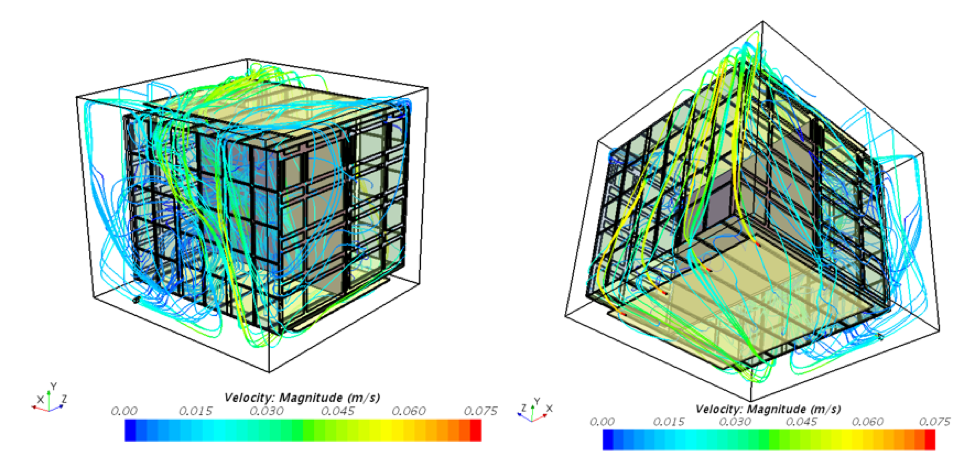
\includegraphics[width=0.9\textwidth]{cisc_cfd_larflow-inlets.png}
\end{dunefigure}



Once the \dword{pdsp} \dword{cfd} model %is able to 
predicts the fluid temperature in the entire cryostat to a reasonable level under different conditions, this model will be extrapolated to  \dword{pddp}  
to produce maps of impurity levels in the \dword{detmodule}. These can be converted easily into electron lifetime maps, which we will %be 
compare to the %data provided by the 
\dword{pddp} purity monitor data. 


%%%%%%%%
\section{Cryogenic Instrumentation}
\label{sec:fdgen-cryo-instr}
%Instrumentation inside the cryostat must ensure that the condition of the \dword{lar} is adequate to operate the \dshort{tpc}.
Instrumentation inside the cryostat must accurately report the condition of the \dword{lar}, so we can ensure that it is adequate for operating the \dshort{tpc}.
This instrumentation includes %devices (the 
purity monitors %)
to check the level of impurity in the argon and %providing 
provide high-precision electron lifetime measurements,
as well as gas analyzers to verify that levels of atmospheric contamination do not drop below certain limits during cryostat purging, cooling, and filling. 
Temperature sensors deployed in vertical arrays and at the top and bottom of the \dword{detmodule} monitor the cryogenics system operation, providing a 
detailed \threed temperature map that helps predict \lar purity across the entire cryostat. The cryogenic instrumentation also includes \lar level monitors and
a system of internal cameras to help find sparks in the cryostat and %for overall 
to monitor the overall cryostat interior. 

The proper placement of purity monitors, thermometers, and liquid-level monitors in the \dword{detmodule} requires %knowing how \dword{lar} behaves 
understanding \lar fluid dynamics, heat and mass transfer, and distribution of impurity concentrations within the cryostat. % in terms of its . 
Both this and % Besides that, 
coherent analysis of the instrumentation data require \dword{cfd} simulation results.


\dword{pdsp} and \dword{pddp} are testing the performance of all cryogenic instrumentation for the \dword{dpmod}, validating the baseline  %\dword{fd} 
design. See Section~\ref{sec:pddp-cryo-valid} for more detail. 


%%%%%%%%%%%%%%%%%%%%%%%%%%%%%%%
\subsection{Thermometers}
\label{sec:fddp-cryo-therm}

%\fixme{ACV: DONE. To be checked by GH/CP}

As discussed in Section \ref{sec:fdgen-cryo-cfd}, a detailed \threed temperature map is important %in 
in monitoring %whether the cryogenic system is functioning correctly and the \lar is uniform.
the cryogenics system for correct functioning and the \lar for uniformity.
Given the complexity and size of purity monitors, they can only be installed where there is sufficient space to provide a local measurement of
\lar purity. 
A direct measurement of the \dword{lar} purity across the entire cryostat is not feasible, but a sufficiently detailed \threed temperature map based on \dword{cfd} simulations can predict the purity. The vertical coordinate is especially important because it will relate closely to the 
\dword{lar} recirculation and uniformity. Monitoring the gas phase in the \dword{dp} technology is also important because the \dword{lem} gain calibration depends on gas temperature. 

 
The baseline sensor distribution 
%and the cryostat ports used to extract cables (with indication of number of cables per port)
%are 
is shown in Figure~\ref{fig:cisc-dp-tsensor-map}. This baseline distribution will evolve as more information becomes available (precise \dword{cfd} simulations, better understanding of cryostat ports, installation interfaces with other groups), but the baseline suffices to establish the overall strategy.

%\fixme{AC: Figure to be replaced, probably by the one with ports provided by David}



High-precision temperature sensors will be distributed near the \dword{tpc} \dword{fc} walls in two ways:
(1) in high density (\(>1\) sensors/\si{m}) vertical arrays %(the so-
(called T-gradient monitors) and (2) in coarser ($\sim$ 1 sensor/\SI{5}{m}) 2D arrays %(the so-
(called individual sensors) at the bottom of the \dword{detmodule}.
The temperature map in the gas phase will be measured using several vertical arrays of standard \dwords{rtd} distributed above the \dwords{crp}.  



Temperature variations inside the cryostat should be very small ($\SI{0.02}{K}$ for the liquid phase (see Figure~\ref{fig:cfd-example}),
so sensors must be cross-calibrated to more than $\SI{0.005}{K}$. Most sensors will be calibrated in the laboratory before installation.
(Installation is described in Section \ref{sec:fdgen-slow-cryo-install-th}.)
Calibrating sensors before installation is the only option for sensors installed in places where space is limited. 
%on the long sides of the detector and the top and bottom of the cryostat, where space is limited.
Given the precision required and the unknown longevity of the sensors, possibly requiring another  calibration after some time, an additional method
will be used for one of the T-gradient monitors based on a movable system that can be used to cross calibrate
the temperature sensors in situ, as described in Section~\ref{sec:fdgen-slow-cryo-dynamic-therm}.

The baseline designs for all thermometer systems have three elements in
common: sensors, cables, and readout system. We plan to use Lake Shore
PT100-series\footnote{Lake Shore Cryotronics\texttrademark{} platinum RTD series,
  \url{https://www.lakeshore.com/}.} %products/cryogenic-temperature-sensors/platinum-rtds/models/Pages/Overview.aspx}.} 
platinum sensors with \SI{100}{\ohm} resistance %are used 
because, in
the temperature range \SIrange{83}{92}{K}, %these particular sensors
they 
show high reproducibility of $\sim\SI{5}{mK}$ and absolute temperature
accuracy of \SI{100}{mK}.  Using a four-wire readout greatly reduces
issues with lead resistance, any parasitic resistances,
connections through the flange, and general electromagnetic noise
pickup. Lakeshore PT102 sensors (see
Figure~\ref{fig:sensor-support}, right) were used in the \dword{35t} prototype
and \dword{pdsp}, % detector, 
giving excellent results. For the inner
readout cables, a custom cable made by Axon\footnote{Axon\texttrademark{} Cable, \url{http://www.axon-cable.com}.}
is the baseline. It
consists of four teflon-jacketed copper wires (AWG28), forming two
twisted pairs, with a metallic external shield and an outer teflon
jacket.
The readout system is described in Section \ref{sec:fdgen-slow-cryo-therm-readout}.

\begin{dunefigure}[Cryostat bolts and temperature sensor support]{fig:sensor-support}
  {Left: bolts at the bottom corner of the cryostat. Right: Lakeshore PT102 sensor mounted on a PCB with an IDC-4 connector.}
  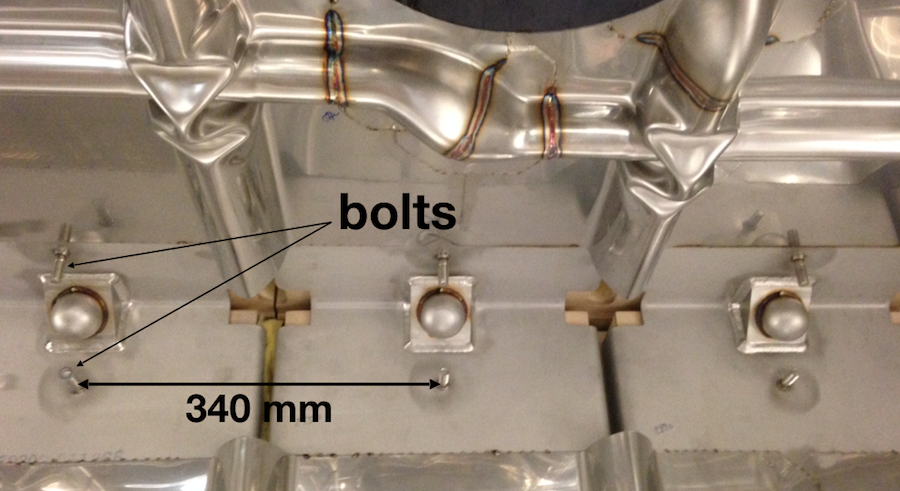
\includegraphics[height=0.2\textwidth]{cisc_cryostat_bolts.png}%
    \hspace{1cm}%
  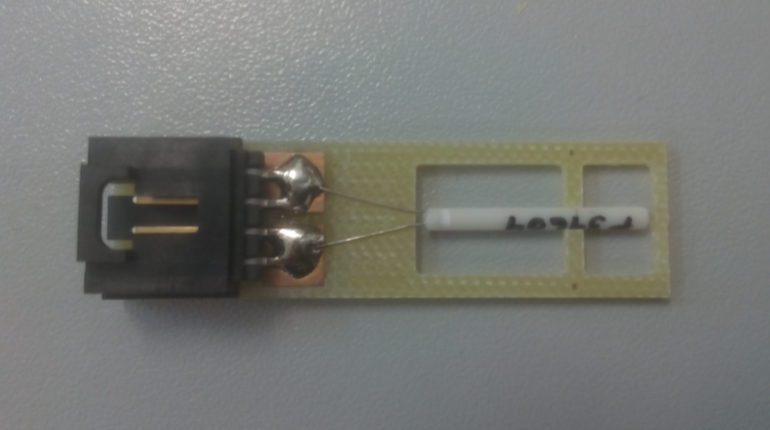
\includegraphics[height=0.2\textwidth]{cisc_tsensor.png}%
\end{dunefigure}


Another set of lower-precision sensors epoxied into the bottom membrane of the cryostat will monitor  cryostat filling in the initial stage.   
Finally, the inner walls and roof of the cryostat will have the same types of sensors to monitor the temperature during \cooldown and filling (W sensors in Figure~\ref{fig:cisc-dp-tsensor-map}).
 
%except for the membrane sensors that may come from Minco.

% % % %
\subsubsection{Dynamic T-gradient monitors}
\label{sec:fdgen-slow-cryo-dynamic-therm}

 Potential differences in sensor readings before and after sensors are installed in a \dword{detmodule} and potential drifts over the lifetime of the %detector 
 module may affect accuracy of the vertical temperature gradient measurement. Thus, to address these concerns, % in a \dword{detmodule}, 
 a dynamic temperature monitor can cross-calibrate  sensor readings %{\em in situ}. 
 \textit{in situ}.
This T-gradient monitor is motorized, allowing vertical movement of the temperature sensor array %in vertical direction while installed 
in the \dword{detmodule}, %. This ability enables 
enabling precise cross-calibration between the sensors %{\em in situ}
in situ, as illustrated in Figure~\ref{fig:sensor-cross-calibration}.  

Cross-calibrations requires several steps. In step 1, the temperature reading  of all sensors is taken at the home (lowest) position of the carrier rod. In  step 2, the stepper motor moves the carrier rod up \SI{25}{cm}. The sensors along the entire  carrier rod are positioned \SI{25}{cm} apart, so when the system moves up \SI{25}{cm}, each sensor is positioned at the height occupied by another sensor in step 1. Then a second temperature reading is taken. Other than the lowest position, this means two temperature measurements are taken at each location with %two 
different sensors. Assuming that the temperature at each location is stable over the few minutes required to make the measurements, %the 
any differences in the temperature readings between the two different sensors would be due to their relative measurement offset. This %temperature readings 
difference is then calculated for all locations.  In step 3, readout differences between pairs of sensors at each location are linked to one another, so each sensor measures the temperature at all heights. In this way, temperature readings from all sensors are cross-calibrated %{\em in situ}
in situ, canceling all possible offsets due to electromagnetic noise or any parasitic resistances that may occur despite the four-point connection to the sensors that should cancel most offsets. These measurements are taken with a very stable current source, which ensures high precision of repeated temperature measurements over time. The dynamic T-monitor operates with a stepper-motor, so measurements are delivered with high spatial resolution. 

\begin{dunefigure}[Principle of cross-calibration with dynamic T-gradient monitor]{fig:sensor-cross-calibration}
  {In step 1, sensor temperature measurements are taken with the T-gradient monitor in the home position. In step 2, the entire system is moved up \SI{25}{cm}, and another set of temperature readings is taken by all sensors. Then, the offsets between pairs of sensors are calculated for each position. In step 3, offsets are linked together, providing cross-calibration of all sensors, to obtain the entire vertical temperature gradient measurement for a single sensor (number 1 in this case). }
  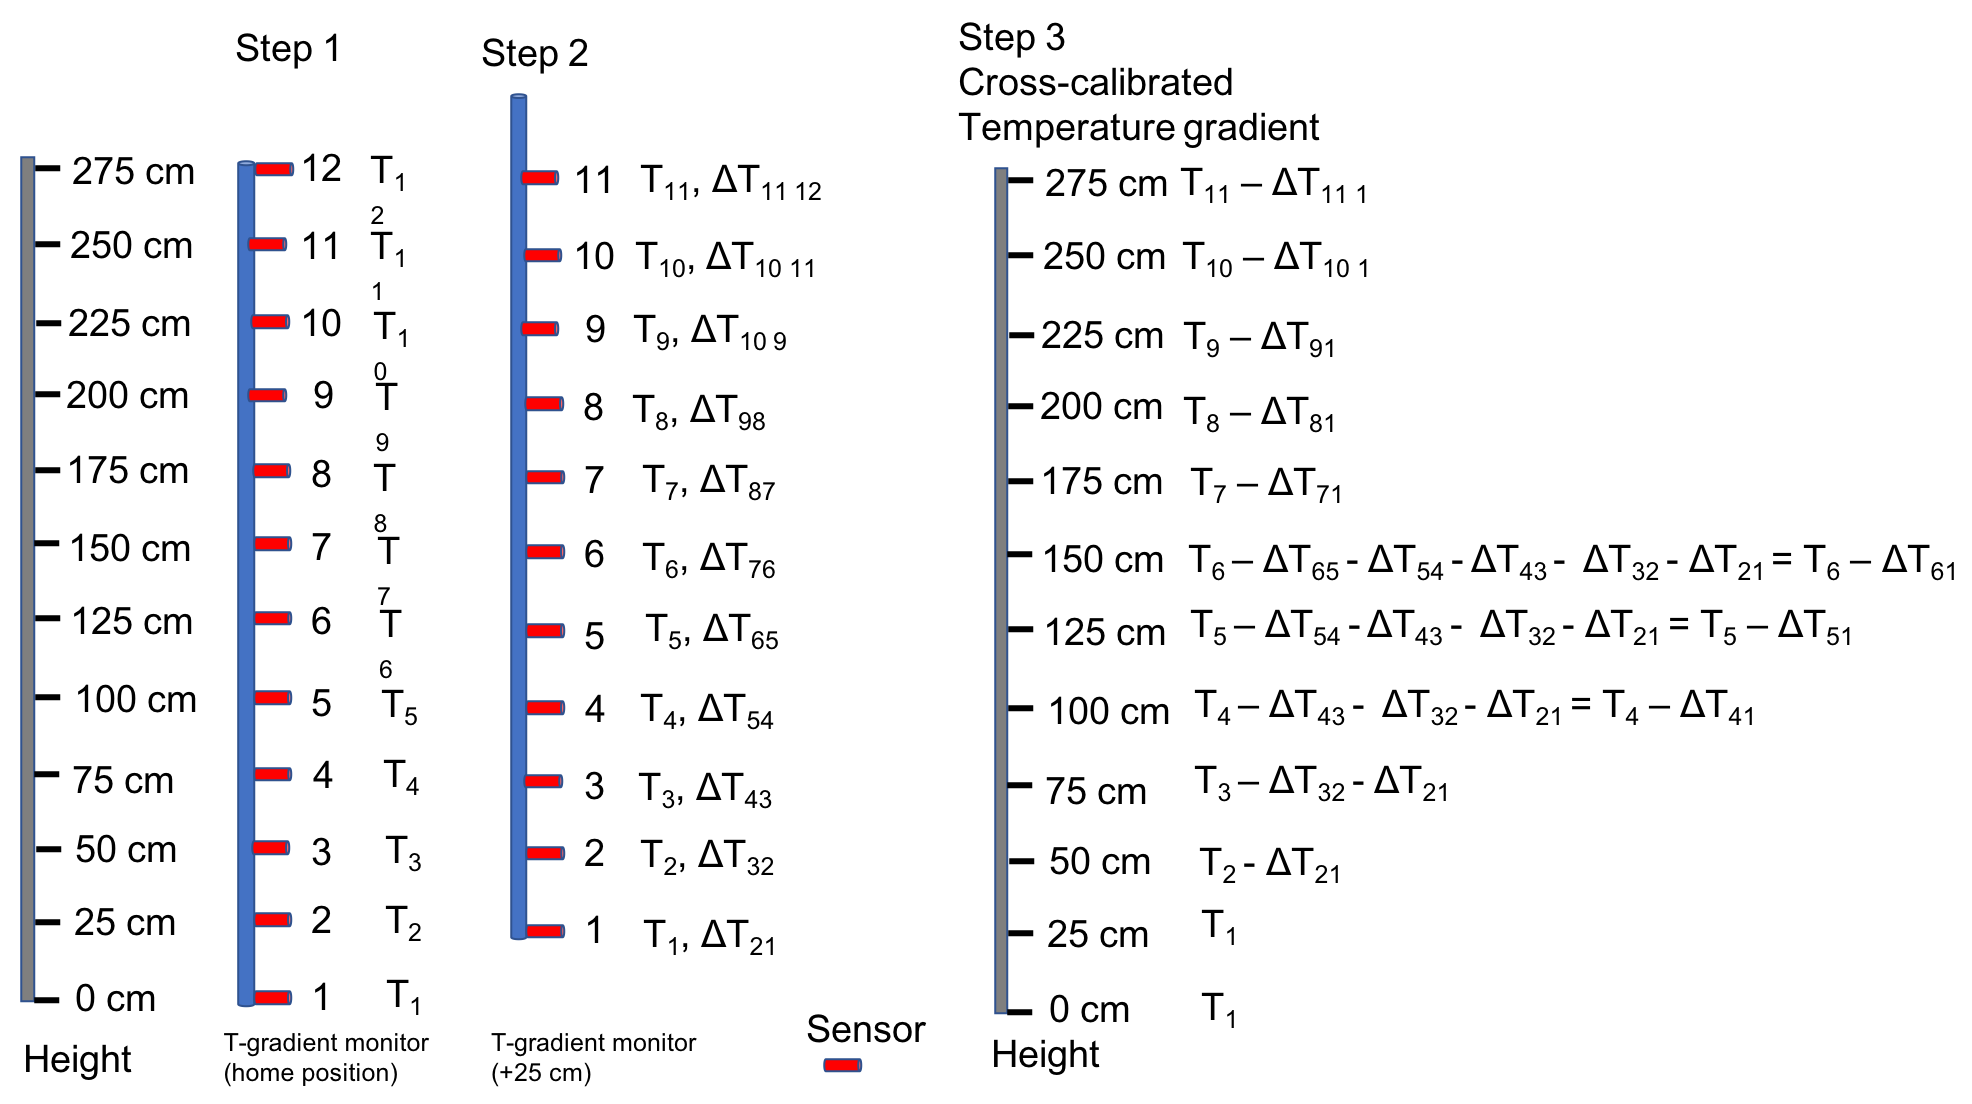
\includegraphics[width=1.0\textwidth]{cisc_cross_calibration_illustration.png}%
\end{dunefigure}


A total of \num{72} sensors will be installed and spaced \SI{25}{cm} apart, although at the top and bottom \SI{1}{m} of the carrier rod, sensor spacing is decreased to \SI{10}{cm}.  
 With the vertical displacement of the system, every sensor can be moved to the nominal position of at least five other sensors, minimizing any risks associated with sensor failure and providing several points of comparison. The total expected motion range of the carrier rod is \SI{1.35}{m}.


This procedure was tested in \dword{pdsp}, where the system was successfully moved up by a maximum of \SI{51}{cm}, allowing cross-calibration of all sensors (22 sensors with \SI{10.2}{cm} spacing at top and bottom and \SI{51}{cm} in the middle). 


Figure~\ref{fig:dynamic_t_pumps-off} shows the temperature profile after calibration when the recirculation pumps are off. Under these conditions the  temperature should be very homogeneous except near the surface. This is indeed what is observed in that figure, demonstrating the reliability of the method.  

\begin{dunefigure}[Temperature profile for dynamic T-Gradient with pumps-off]{fig:dynamic_t_pumps-off}
  {Temperature profile as measured by the dynamic T-gradient monitor after cross-calibration when the recirculation pumps are off. Temperature variation is approximately \SI{3}{mK} except close to the top and the gas phase interface, as expected.}
  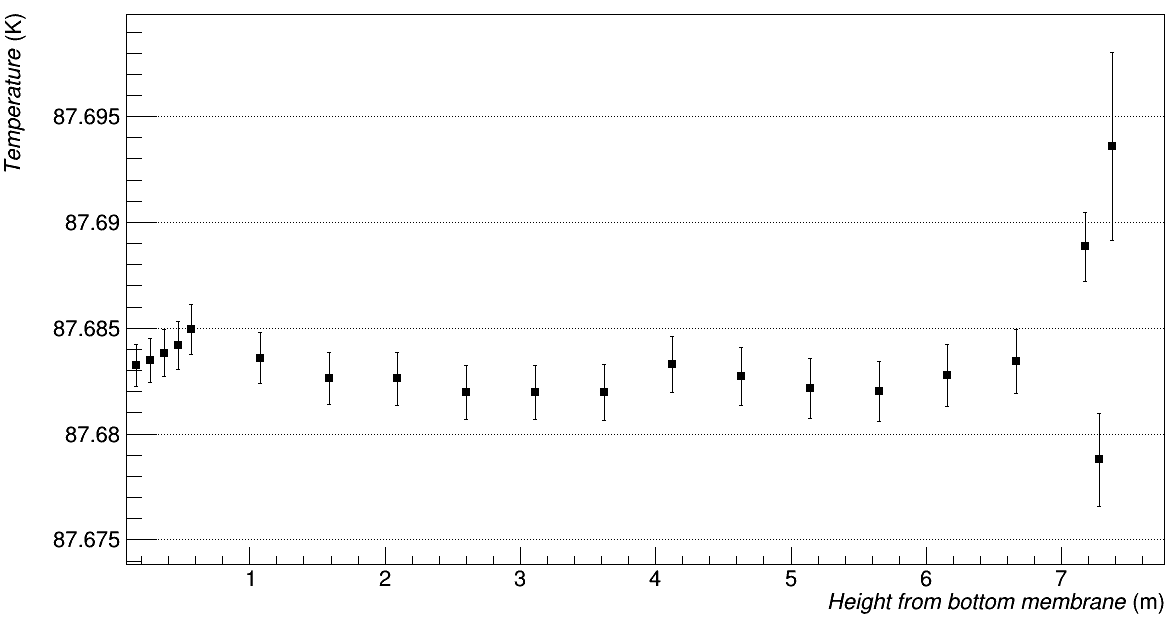
\includegraphics[width=0.6\textwidth]{cisc_dynamic_t_pumps-off.png}%
\end{dunefigure}



A dynamic T-gradient monitor has three parts: a carrier rod on which sensors are mounted; an enclosure above the cryostat housing space that allows the carrier rod to move vertically  \SI{1.5}{m} over its lowest location; and the motion mechanism. The motion mechanism is a stepper motor connected through a ferrofluidic dynamic seal to a gear and pinion motion mechanism. The sensors have two pins soldered to a \dword{pcb}. 
%\fixme{maybe add gloss term}
Two wires are individually soldered to the common soldering pad for each pin.  A cutout in the \dword{pcb} around the sensor allows free flow of argon for more accurate temperature readings.  Stepper motors typically have very fine steps that allow highly precise positioning of the sensors.  Figure~\ref{fig:fd-slow-cryo-dt-monitor-overview} shows the overall design of the dynamic T-gradient monitor. % with the sensor carrier rod, enclosure above the cryostat, and stepper motor mounted on the side of the enclosure. 
The enclosure has two parts connected by a six-cross flange. One side of this flange will be used for signal wires, another will be used as a viewing window, and the two other ports will be spares. Figure~\ref{fig:fd-slow-cryo-sensor-mount}, left, shows the \dword{pcb} mounted on the carrier rod and the sensor mounted on the \dword{pcb} along with the four point connection to the signal readout wires. %Finally, 
Figure~\ref{fig:fd-slow-cryo-sensor-mount}, right, shows the stepper motor mounted on the side of the rod enclosure. The motor remains outside the enclosure, at room temperature, %and 
as do its power and control cables. % also remain outside.

\begin{dunefigure}[Dynamic T-gradient monitor overview]{fig:fd-slow-cryo-dt-monitor-overview}
  {%An overview 
  A schematic of the dynamic T-gradient monitor.}
% 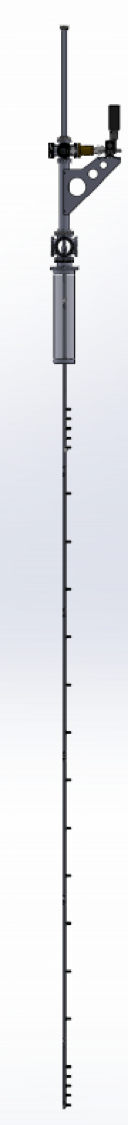
\includegraphics[width=0.11\textwidth,angle=90]{cisc_DTOverview.png}
 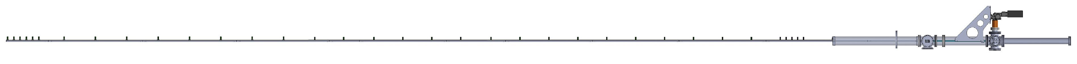
\includegraphics[width=0.95\textwidth,angle=0]{cisc_DynamicProfiler.png}
\end{dunefigure}
\begin{dunefigure}[Sensor-cable assembly for dynamic T-gradient monitor]{fig:fd-slow-cryo-sensor-mount}
  {Left: Sensor mounted on a PCB board, and PCB board mounted on the rod. Right:
    The driving mechanism of the dynamic T-gradient monitor consisting of a stepper motor driving the pinion and gear linear motion mechanism. }
  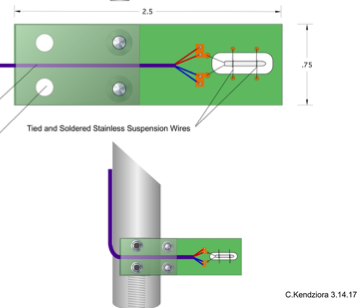
\includegraphics[width=0.40\textwidth]{cisc_DTSensorMount.png}
  \hspace{3cm}%
  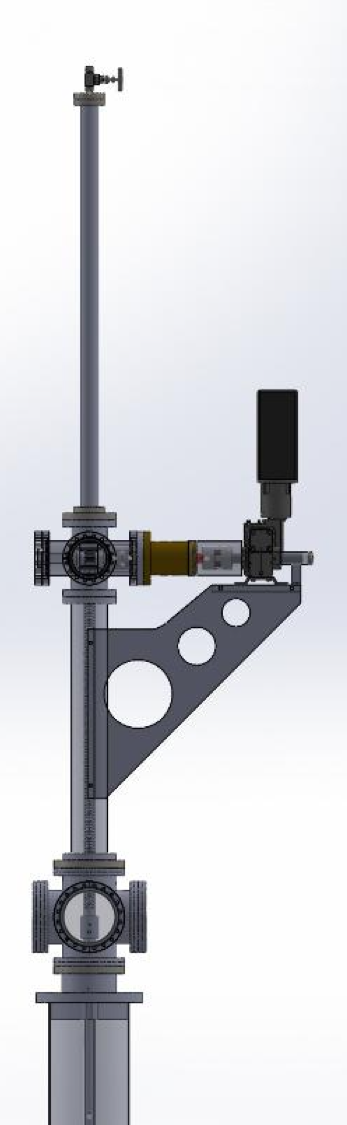
\includegraphics[width=0.12\textwidth]{cisc_DTMotor.png}
\end{dunefigure}

% % % %

\subsubsection{Static T-gradient monitors}
\label{sec:fdgen-slow-cryo-static-therm}

Several vertical arrays of high-precision temperature sensors cross-calibrated in the laboratory will be installed behind the lateral \dwords{fc}.  

The baseline design assumes six arrays with \num{24} sensors each. 
Spacing between sensors
is \SI{40}{cm} at the top and bottom and \SI{80}{cm} in the middle area.

As shown in Figure~\ref{fig:pd_static_t_results} a configuration with \num{48} sensors was appropriate in \dword{pdsp}, as it should be in the \dword{dpmod} where the expected total gradient is no larger than in \dword{pdsp} (see Figure~\ref{fig:cfd-example}). 

\begin{dunefigure}[ProtoDUNE-SP Static T-gradient results]{fig:pd_static_t_results}{
 Left: Temperature profile as measured by the static T-gradient monitor for two different calibration methods. Right: Distribution of the difference between both methods.}
  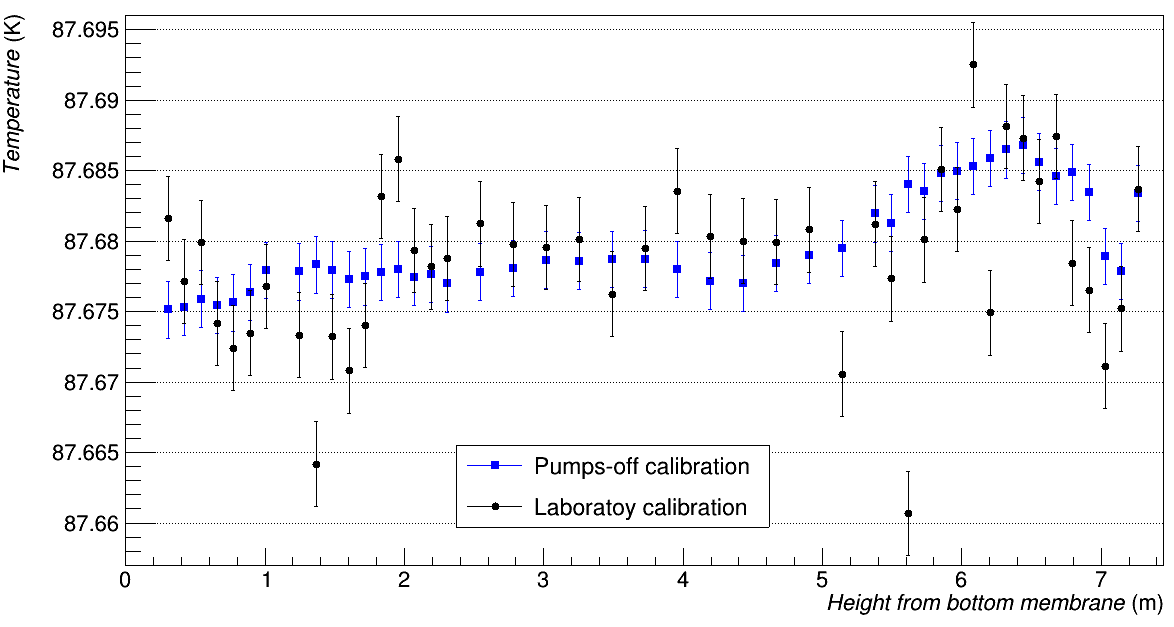
\includegraphics[height=0.34\textwidth]{cisc_static_t_profiles.png}%
  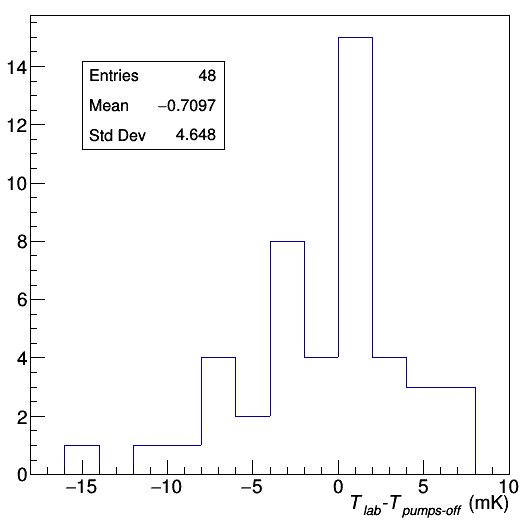
\includegraphics[height=0.34\textwidth]{cisc_static_t_calib_diff.png}%
\end{dunefigure}



Sensors will be cross-calibrated in the laboratory using a controlled environment and a high-precision readout system, described in Section \ref{sec:fdgen-slow-cryo-therm-readout}.

The accuracy of the calibration for \dword{pdsp} was estimated to be $\SI{2.6}{mK}$ (see Figure~\ref{fig:Trepro}). Figure~\ref{fig:pd_static_t_results} shows the preliminary results of the analysis of \dword{pdsp} static T-gradient monitor data. The temperature profile was computed using both the laboratory calibration and the so-called ``in-situ pump-off'' calibration, which consists %in 
of estimating the offsets between sensors assuming the temperature of \lar in the cryostat is homogeneous when the re-circulation pumps are off. (The validity of this method is demonstrated in Section~\ref{sec:fdgen-slow-cryo-dynamic-therm}.)  
The \dword{rms} of the difference between both methods is $\SI{4.6}{mK}$, slightly more than the value quoted above for the accuracy of laboratory calibration, due to the presence of a few outliers (under investigation) and the imperfect assumption of homogeneous temperature when pumps are off (see Figure~\ref{fig:dynamic_t_pumps-off}).  

\begin{dunefigure}[Temperature sensor resolution and reproducibility]{fig:Trepro}{
 Left:   Temperature offset between two sensors as a function of time for four independent immersions in LAr. The reproducibility of those sensors, defined as the RMS of the mean offset in the flat region, is $\sim\,\SI{1}{mK}$,
    The resolution for individual measurements, defined as the RMS of one offset in the flat region, is more than \SI{0.5}{mK}. Right: Difference between the mean offset obtained with two independent calibration methods for the 51 calibrated sensors. The standard deviation of this distribution is interpreted as precision of the calibration.}
  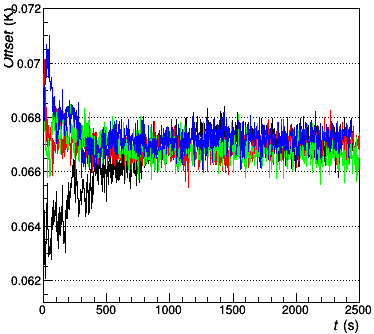
\includegraphics[height=0.44\textwidth]{cisc_tsensor_calib.png}%
  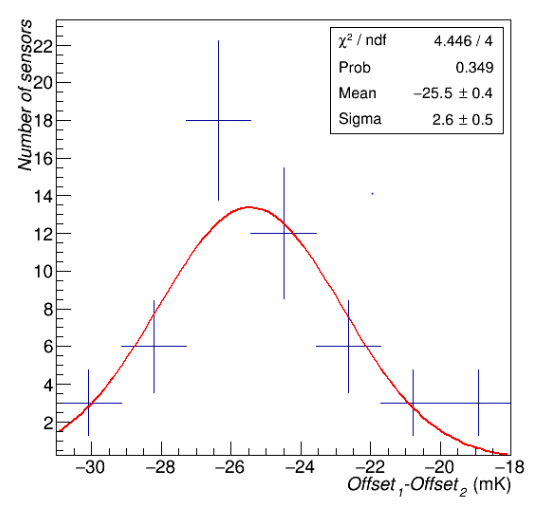
\includegraphics[height=0.45\textwidth]{cisc_tsensor_calib2.png}%
\end{dunefigure}



Figure~\ref{fig:cisc-static-tgradient} shows the baseline mechanical design of
the static T-gradient monitor. Two vertical strings are anchored at the top and bottom corners of the cryostat
using the available M10 bolts (see Figure~\ref{fig:sensor-support}, left). One string routes the cables while the other,
separated from the first by \SI{150}{mm},  supports the temperature sensors and the individual Faraday cages. 
Given the height of the cryostat, an intermediate anchoring point might be needed to reduce swinging. To reduce the effect of shrinkage in the strings under cryogenic conditions and to guarantee that the same tension is always applied, springs will be made of materials with low coefficients of linear thermal expansion, like carbon fiber or invar. A special spring could be also used. A prototype is being built at \dword{ific}, where the full system will be mounted using two dummy cryostat corners.  
\begin{dunefigure}[Conceptual design of the static T-gradient monitor]
{fig:cisc-static-tgradient}
  {Conceptual design of the static T-gradient monitor.}
  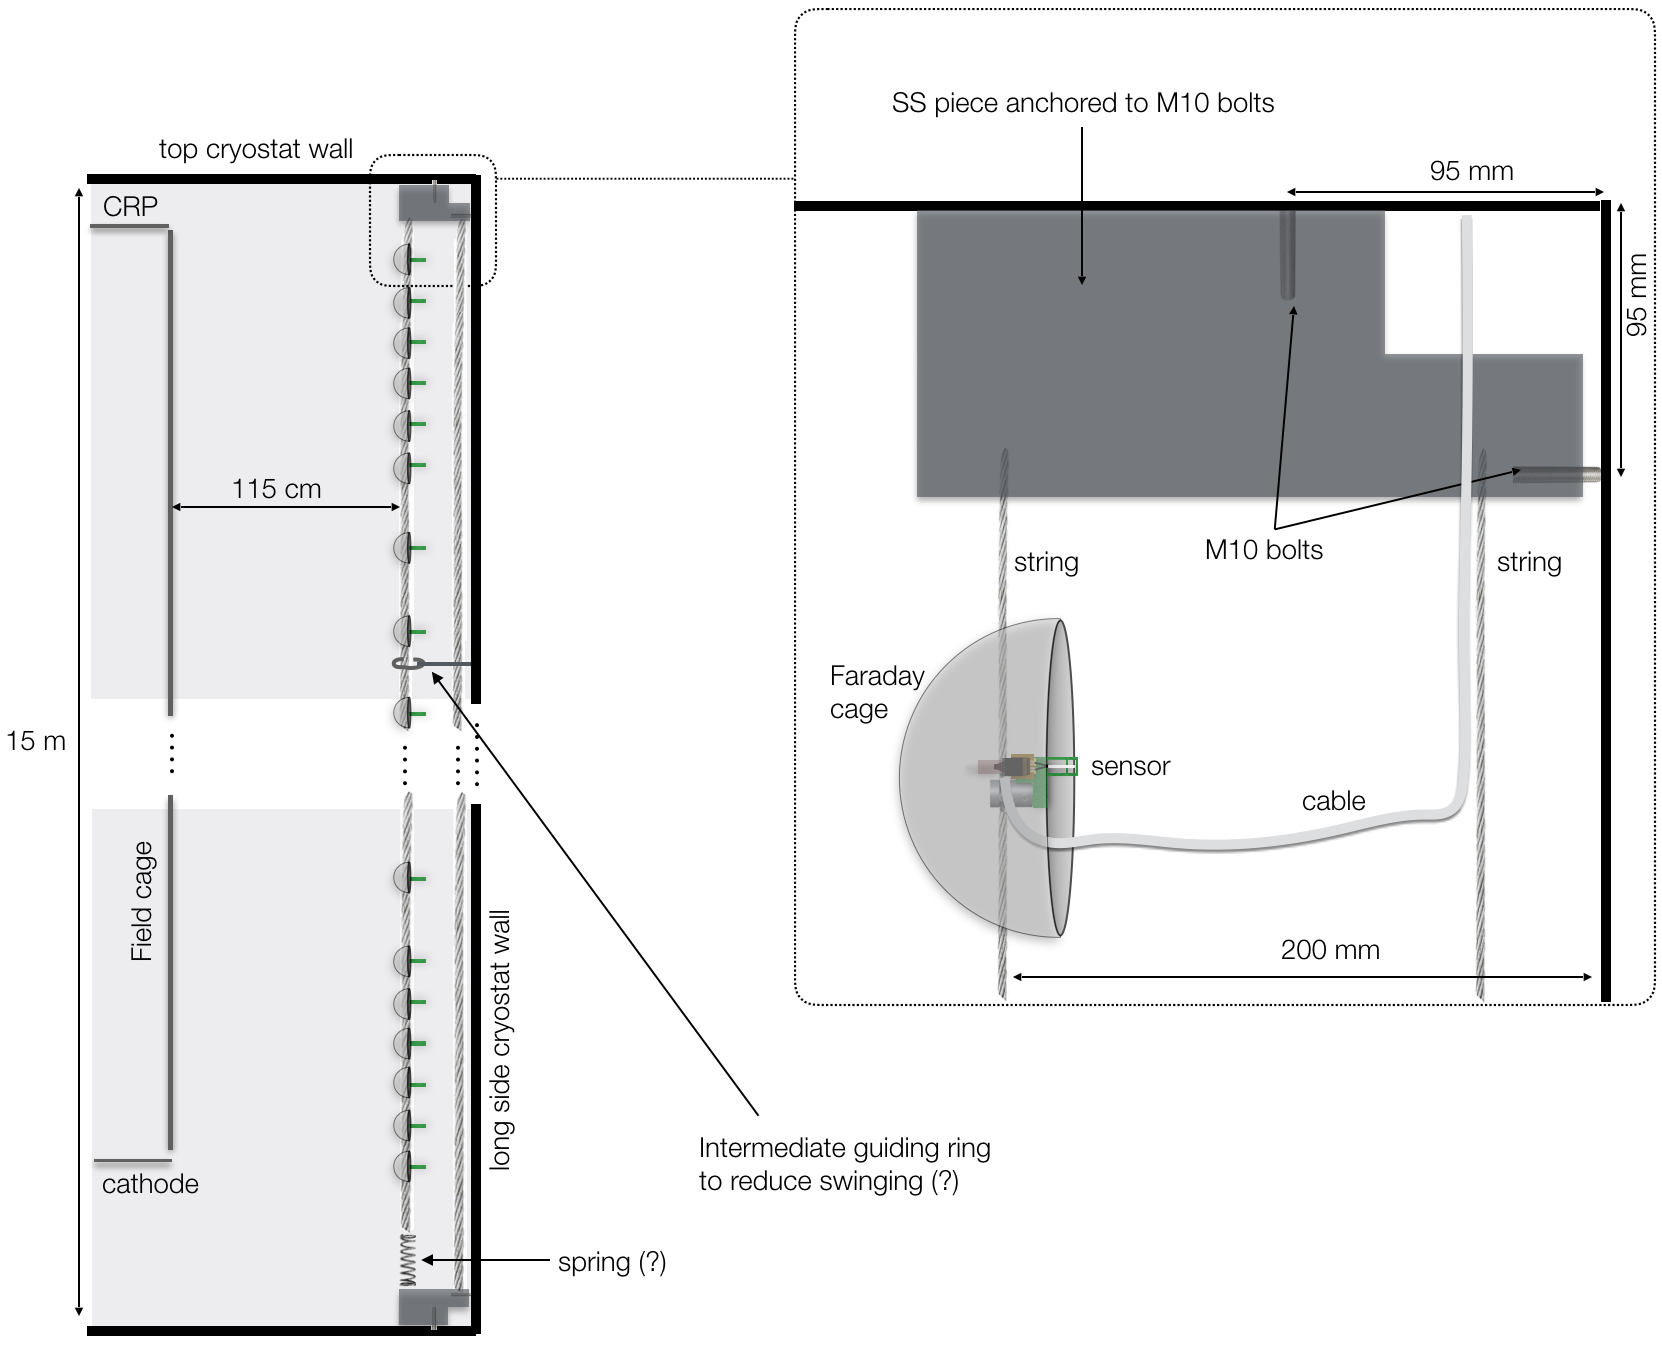
\includegraphics[width=0.8\textwidth]{cisc_dp_static_tgradient.png}
\end{dunefigure}


Figure~\ref{fig:sensor-support}, right, shows the baseline design of the ($52\times \SI{15}{mm^2}$) 
PCB support for temperature sensors with an IDC-4 male connector. %It is . 

A narrower connector (with two rows of two pins each) is being studied. This alternative design would reduce the width of the \dword{pcb} assembly and allow more sensors to be calibrated simultaneously. Each four-wire cable from the sensor to the flange will have an IDC-4 female connector on the sensor end; the flange end of the cable will be soldered or crimped to the appropriate connector, whose type and number of pins  depend on the final design of the \dword{dss} ports that will be used to extract the cables. SUBD-25 connectors were used in \dword{pdsp}.


% % % %
\subsubsection{Individual Temperature Sensors}
\label{sec:fdgen-slow-cryo-individual-therm}

T-gradient monitors will be complemented by a coarser 2D array (every \SI{5}{m}) of precision sensors at the bottom of the \dword{detmodule}, as shown in Figure~\ref{fig:cisc-dp-tsensor-map}. These sensors could  use the cryogenic pipes as a support structure following the \dword{pdsp} design. An alternative design using the support structure for \dwords{pd} is also under consideration.  

As in \dword{pdsp}, another set of standard sensors will be evenly distributed and epoxied to the bottom membrane. They will detect the presence of \lar when cryostat filling starts. Finally, two vertical arrays of standard sensors will be epoxied to the lateral walls in two opposite vertical corners, spaced \SI{102}{cm} apart (every three corrugations), to monitor the cryostat membrane temperature during \cooldown and filling. 

 
Whereas in \dword{pdsp}, cables were routed individually (without touching neighboring cables or any metallic elements) to prevent grounding loops in case the outer Teflon jacket broke, such a failure is very unlikely. Thus, in the \dwords{detmodule}, cables will be routed in bundles, simplifying the design enormously. 
Cable bundles of several sizes will be configured using custom made Teflon 
pieces  
that will be anchored to different cryostat and detector elements to route cables from sensors to the assigned cryostat ports. For sensors at the bottom (on pipes/\dwords{pd} and floor), cables will be routed towards the bottom horizontal corner of the cryostat using stainless steel split clamps anchored to pipes (successfully prototyped in \dword{pdsp}) and from there, to the top of the cryostat using vertical strings (as with static T-gradient monitors). 

Sensors on the walls will use bolts in the vertical corners for cable routing. 

For all individual sensors, \dword{pcb} sensor support, cables, and connection to the flanges will be the same as for the T-gradient monitors. 
  



\subsubsection{Vertical arrays in gas phase}
\label{sec:fdgen-slow-cryo-static-therm-gass}

The temperature map in the gas is especially important for the \dword{dp} technology. 
As in \dword{pddp}, the region immediately above (about \SI{40}{cm}) the \dwords{crp} will be instrumented with vertical arrays of temperature sensors.  %The baseline design foresees for each of these arrays eight standard \dwords{rtd} with increasing pitch with height above the \dword{crp}, 
In the baseline design, each array is a vertical distribution of eight standard \dwords{rtd} above the \dword{crp}, in which the distance between them increases with height, as shown in Figure~\ref{fig:cisc-tsensor-gas} for the device installed in \dword{pddp}.  Twenty (20) of these arrays would be distributed throughout the top of the cryostat. Unlike the liquid, where the temperature gradient is not larger than \SI{10}{mK}, the temperature in the gas changes very rapidly with height, and a relative precision of \SI{0.1}{K} is sufficient for those sensors. Thus, standard \dwords{rtd} with calibration can be used.    

\begin{dunefigure}[Arrays in gas phase]{fig:cisc-tsensor-gas}
  {Vertical array of temperature sensors in \dword{pddp}.
  }
 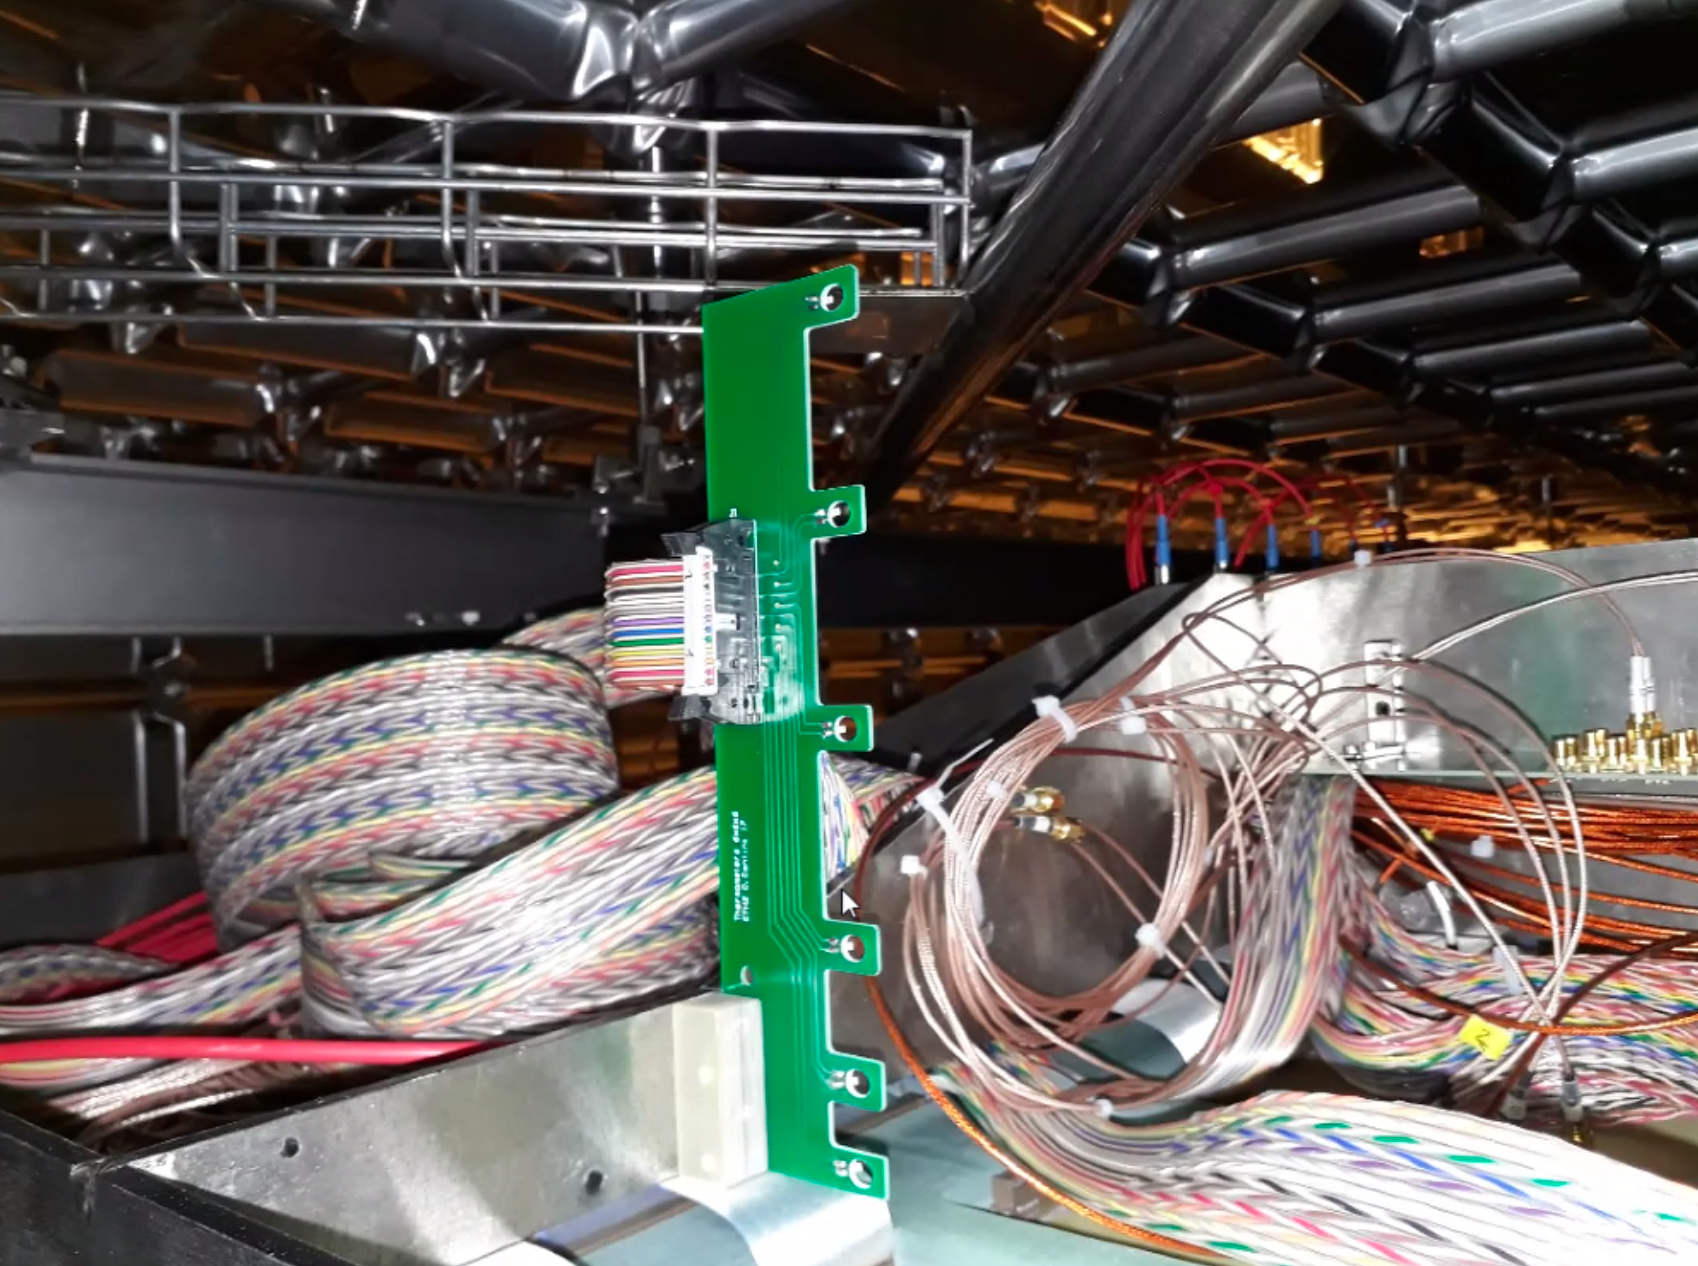
\includegraphics[width=0.8\textwidth,angle=0]{cisc_dp_tsensor_gas}
\end{dunefigure}

\subsubsection{Analysis of temperature data in \dword{pdsp}}
\label{sec:fdgen-slow-cryo-temp-ana}


Temperature data from \dword{pdsp} has been recorded since \dword{lar} filling %started 
in August 2018. The analysis of this data and the comparison with \dword{cfd} simulations is actively underway, but interesting preliminary results are available and will be described below. Figure~\ref{fig:pd_inst_map} shows the distribution of temperature sensors in the \dword{pdsp} cryostat.  

\begin{dunefigure}[ProtoDUNE-SP instrumentation map]{fig:pd_inst_map}{Distribution of temperature sensors in the \dword{pdsp} cryostat. Notice that four of the bottom sensors are located right above the LAr inlets. Purity monitors and level meters are also indicated. }
  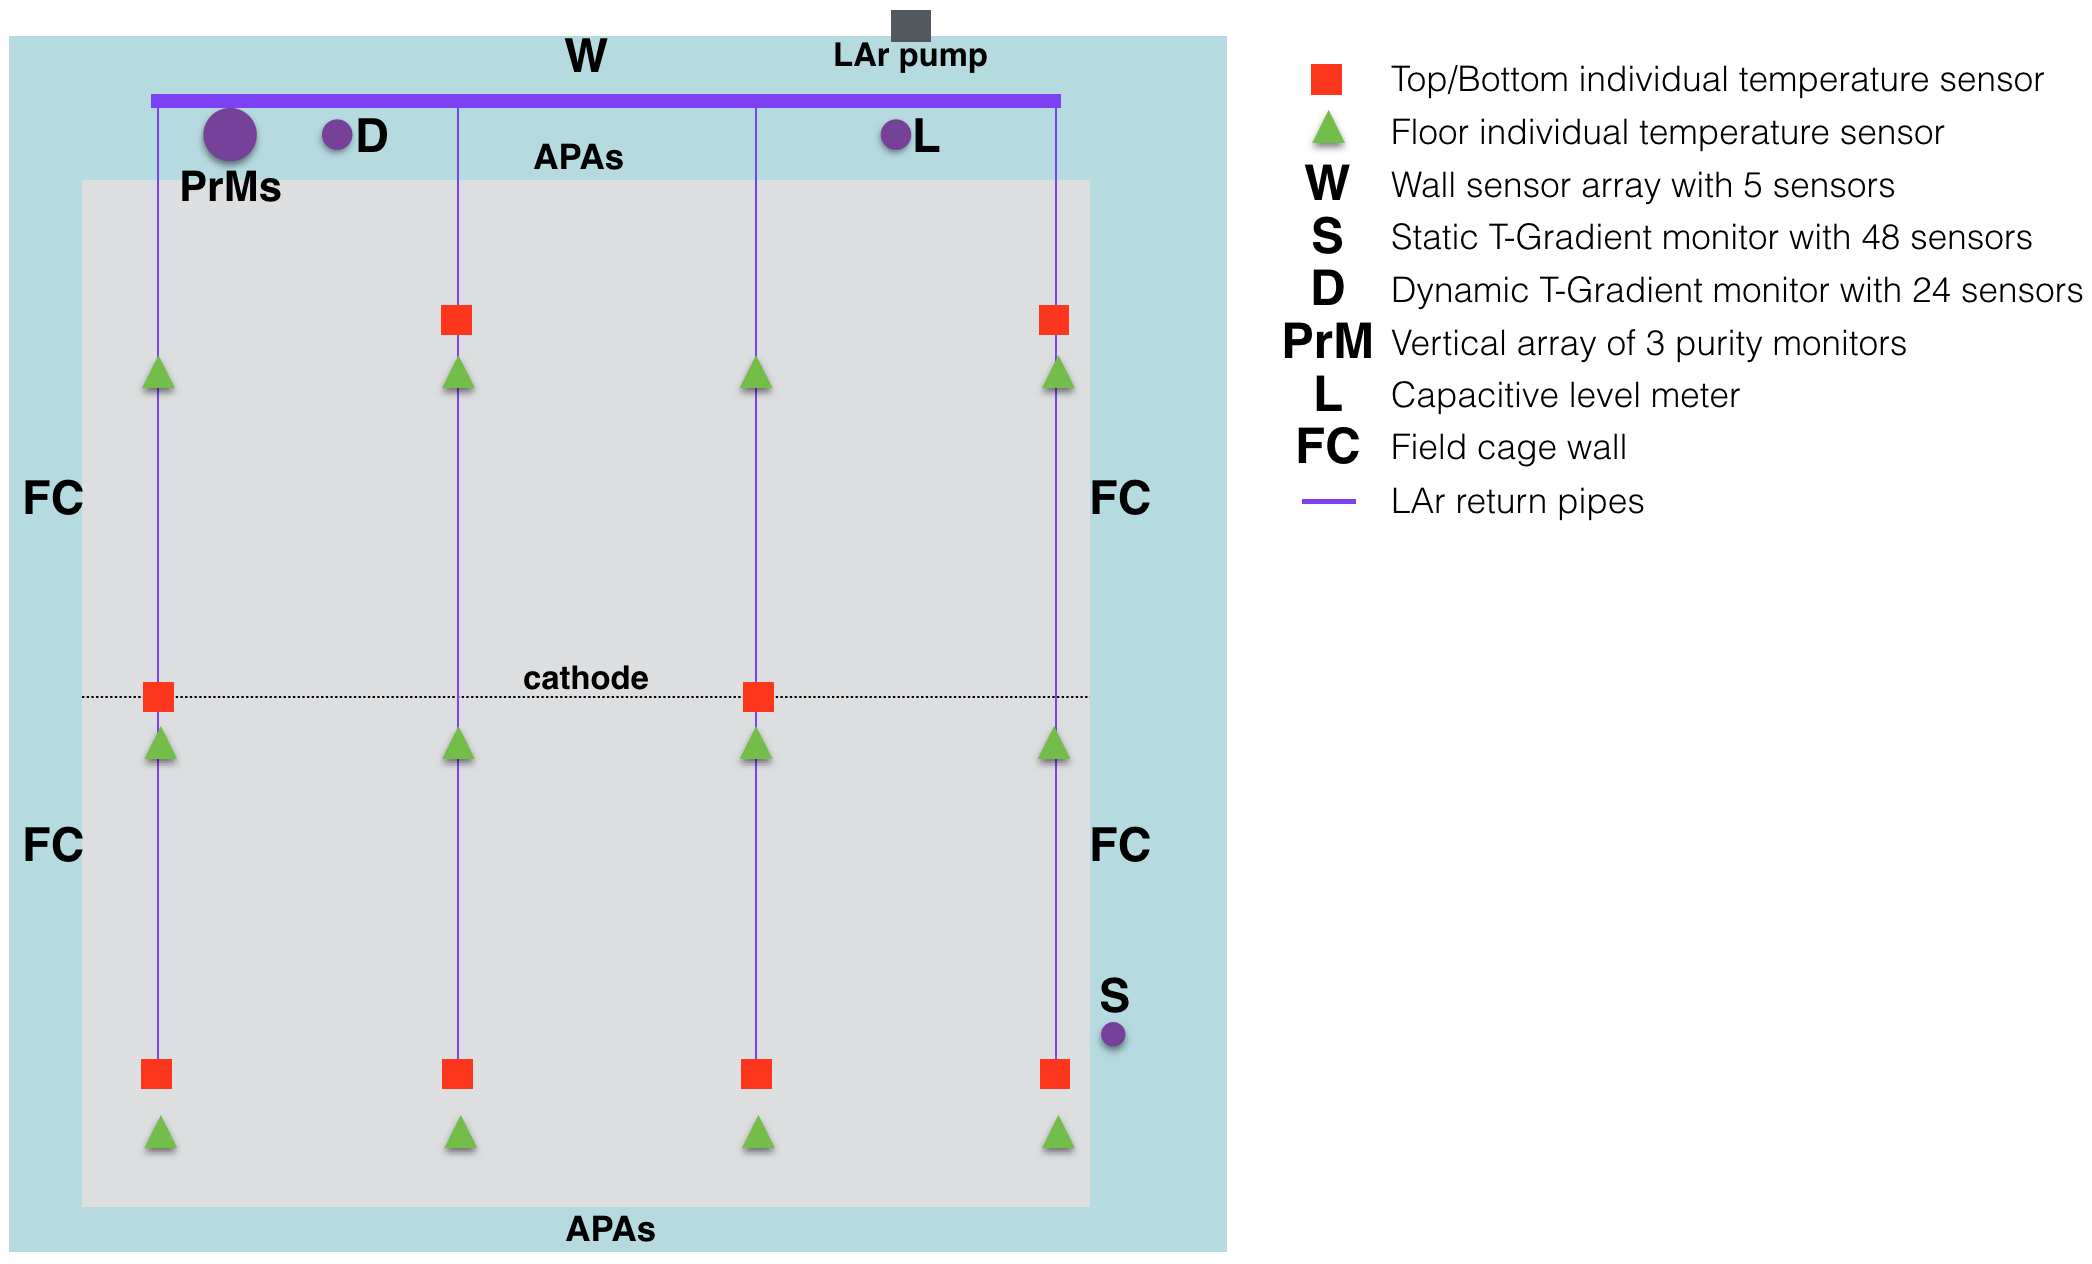
\includegraphics[width=0.7\textwidth]{cisc_pdsp_instrumentation.png}%
\end{dunefigure}


All precision temperature sensors (for the static and dynamic T-gradient monitors,  and the 2D arrays at top and bottom) were calibrated in the laboratory prior to installation. However, since the calibration method was still under development when those sensors 
%had to be 
were installed, this calibration was only satisfactory (2.6 mK precision) for the static T-gradient monitor, whose sensors were calibrated the last and  plugged in just few days prior to installation in the cryostat. In section~\ref{sec:fdgen-slow-cryo-static-therm}, an additional calibration method, the so called {\it pumps-off calibration}, has been described and the agreement with the laboratory calibration was proved (see Figure~\ref{fig:pd_static_t_results}). Since this is the only reliable calibration for individual sensors, this method will be used for the data analysis presented in this section, for all sensors except for the dynamic T-gradient monitor, whose calibration based on the movable system is more precise (see Sec.~\ref{sec:fdgen-slow-cryo-dynamic-therm}). 


Figure~\ref{fig:pd_tgradient_results} shows the vertical temperature profiles as measured by the dynamic and static T-gradient monitors at a given moment in time (10 minutes in May 2019). The stability of those profiles has been carefully studied: the relative variation between any two sensors on the same profiler is below 3 mK along the entire data taking, probing that the shape of the profiles is nearly constant in time. In Figure~\ref{fig:pd_tgradient_results} one immediately observes that the shapes of the two profiles are similar, with a bump at 6.2 m, but the magnitude of %the 
variation of the static profile almost doubles %the one of 
compared to the dynamic profile. This effect is attributed to the fact that the dynamic T-gradient monitor is on the path of the \lar flow, which makes the temperature more uniform, while the static profiler is on the side.  

\begin{dunefigure}[ProtoDUNE-SP T-gradient results]{fig:pd_tgradient_results}{Temperature profiles measured by the T-gradient monitors and comparison to the \dword{cfd} model with different boundary conditions. Left: dynamic T-gradient monitor; Right: Static T-gradient monitor.}
  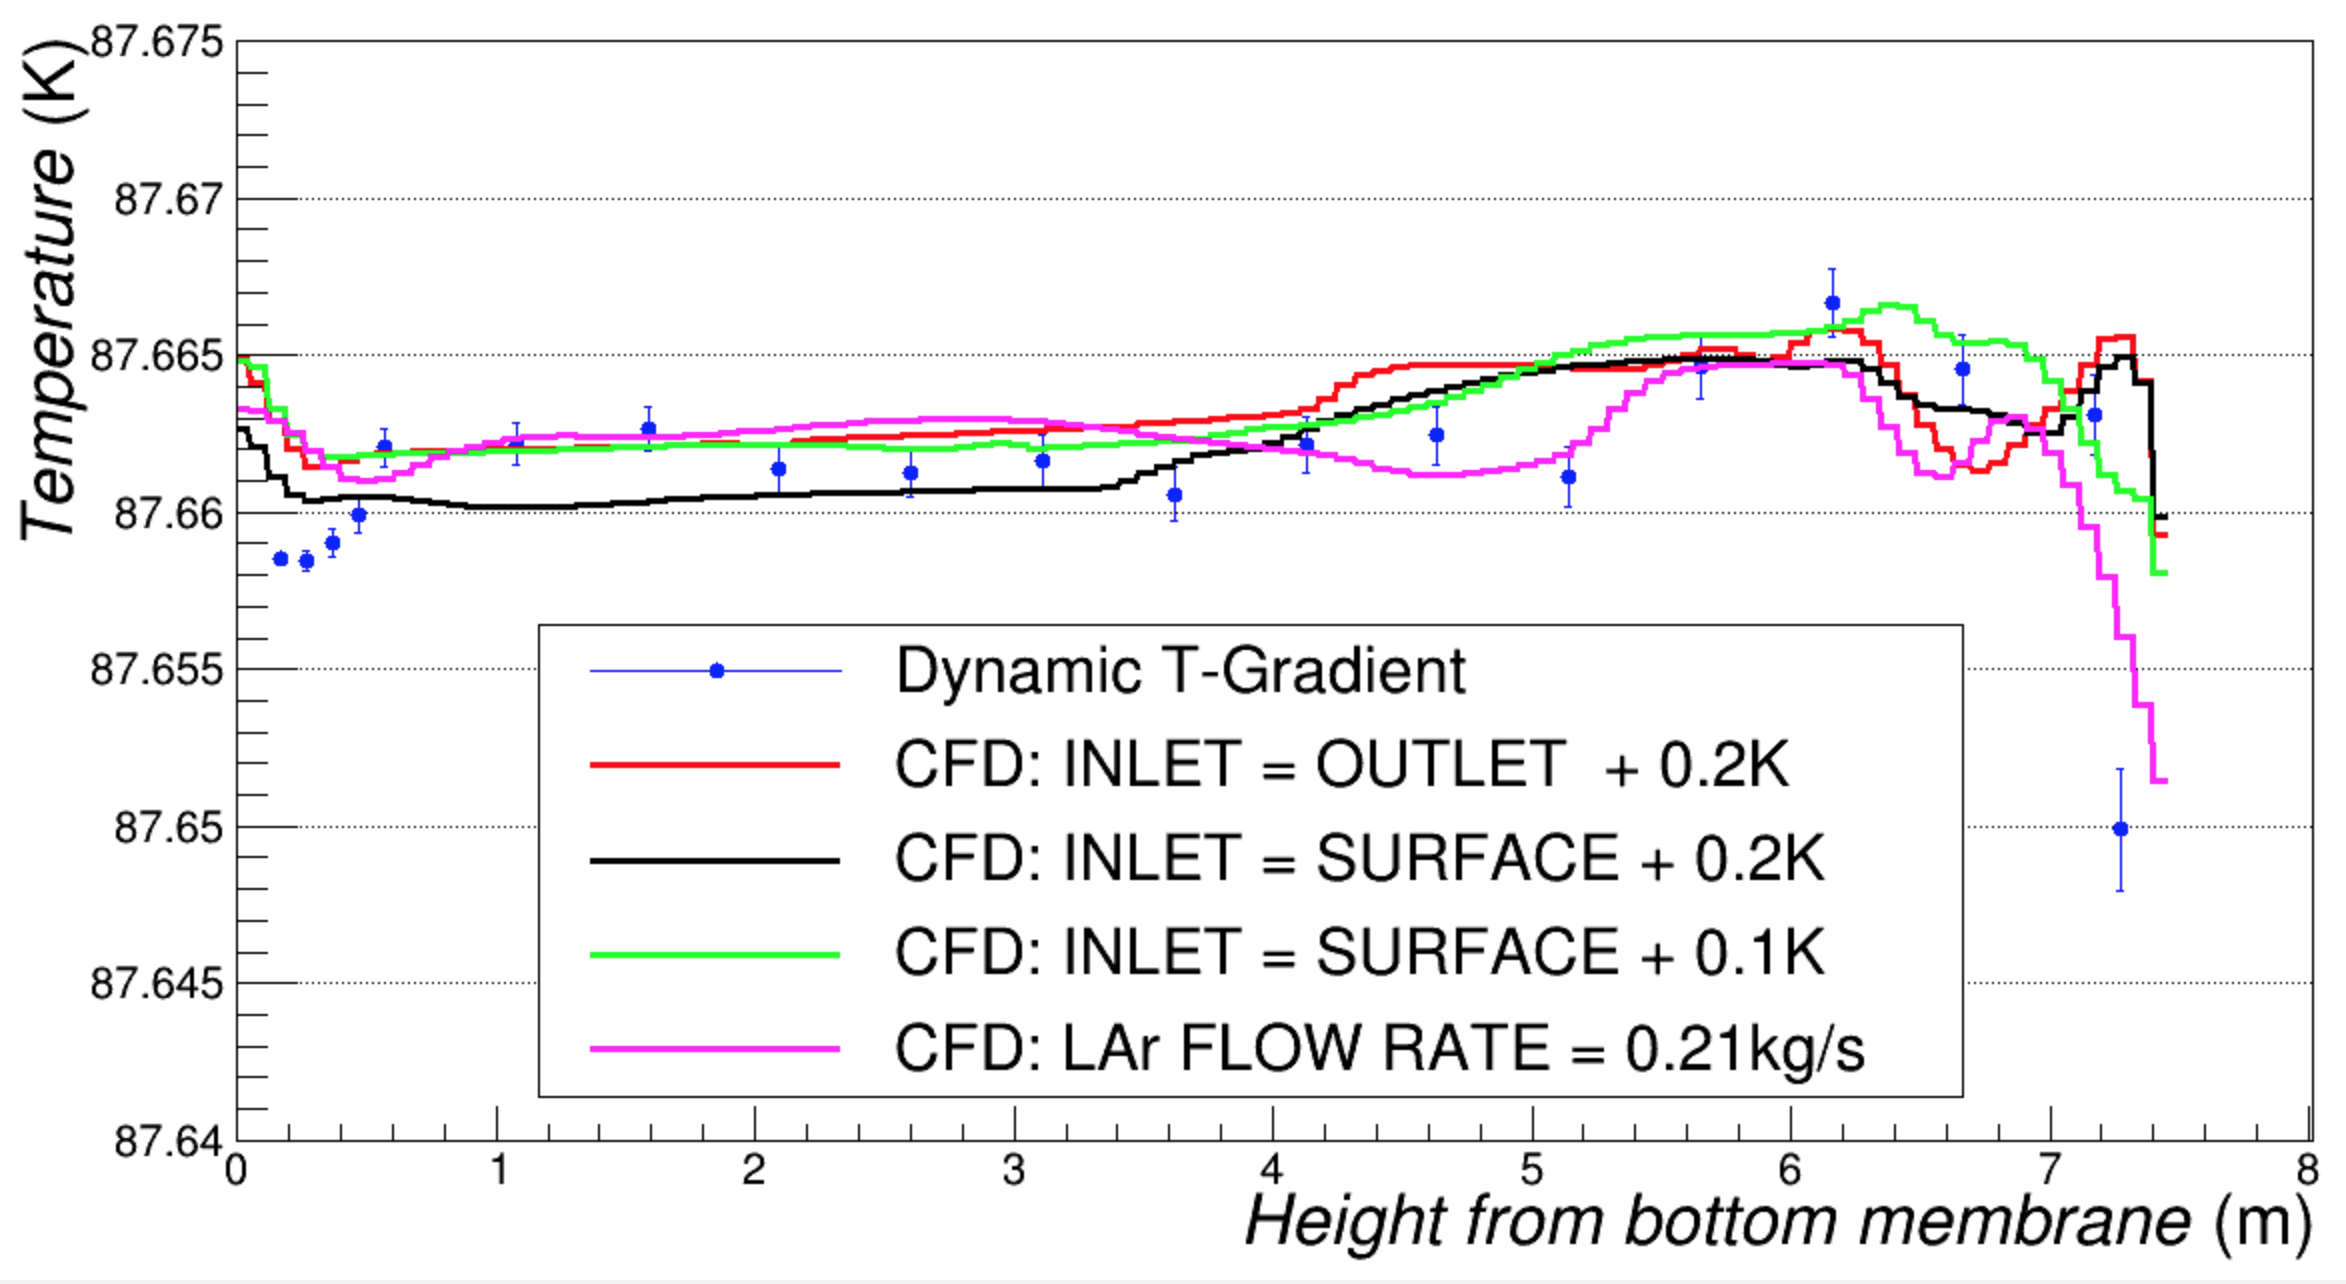
\includegraphics[width=0.5\textwidth]{cisc_dynamic_cfd_data.png}%
%  \hspace*{0.3cm}
  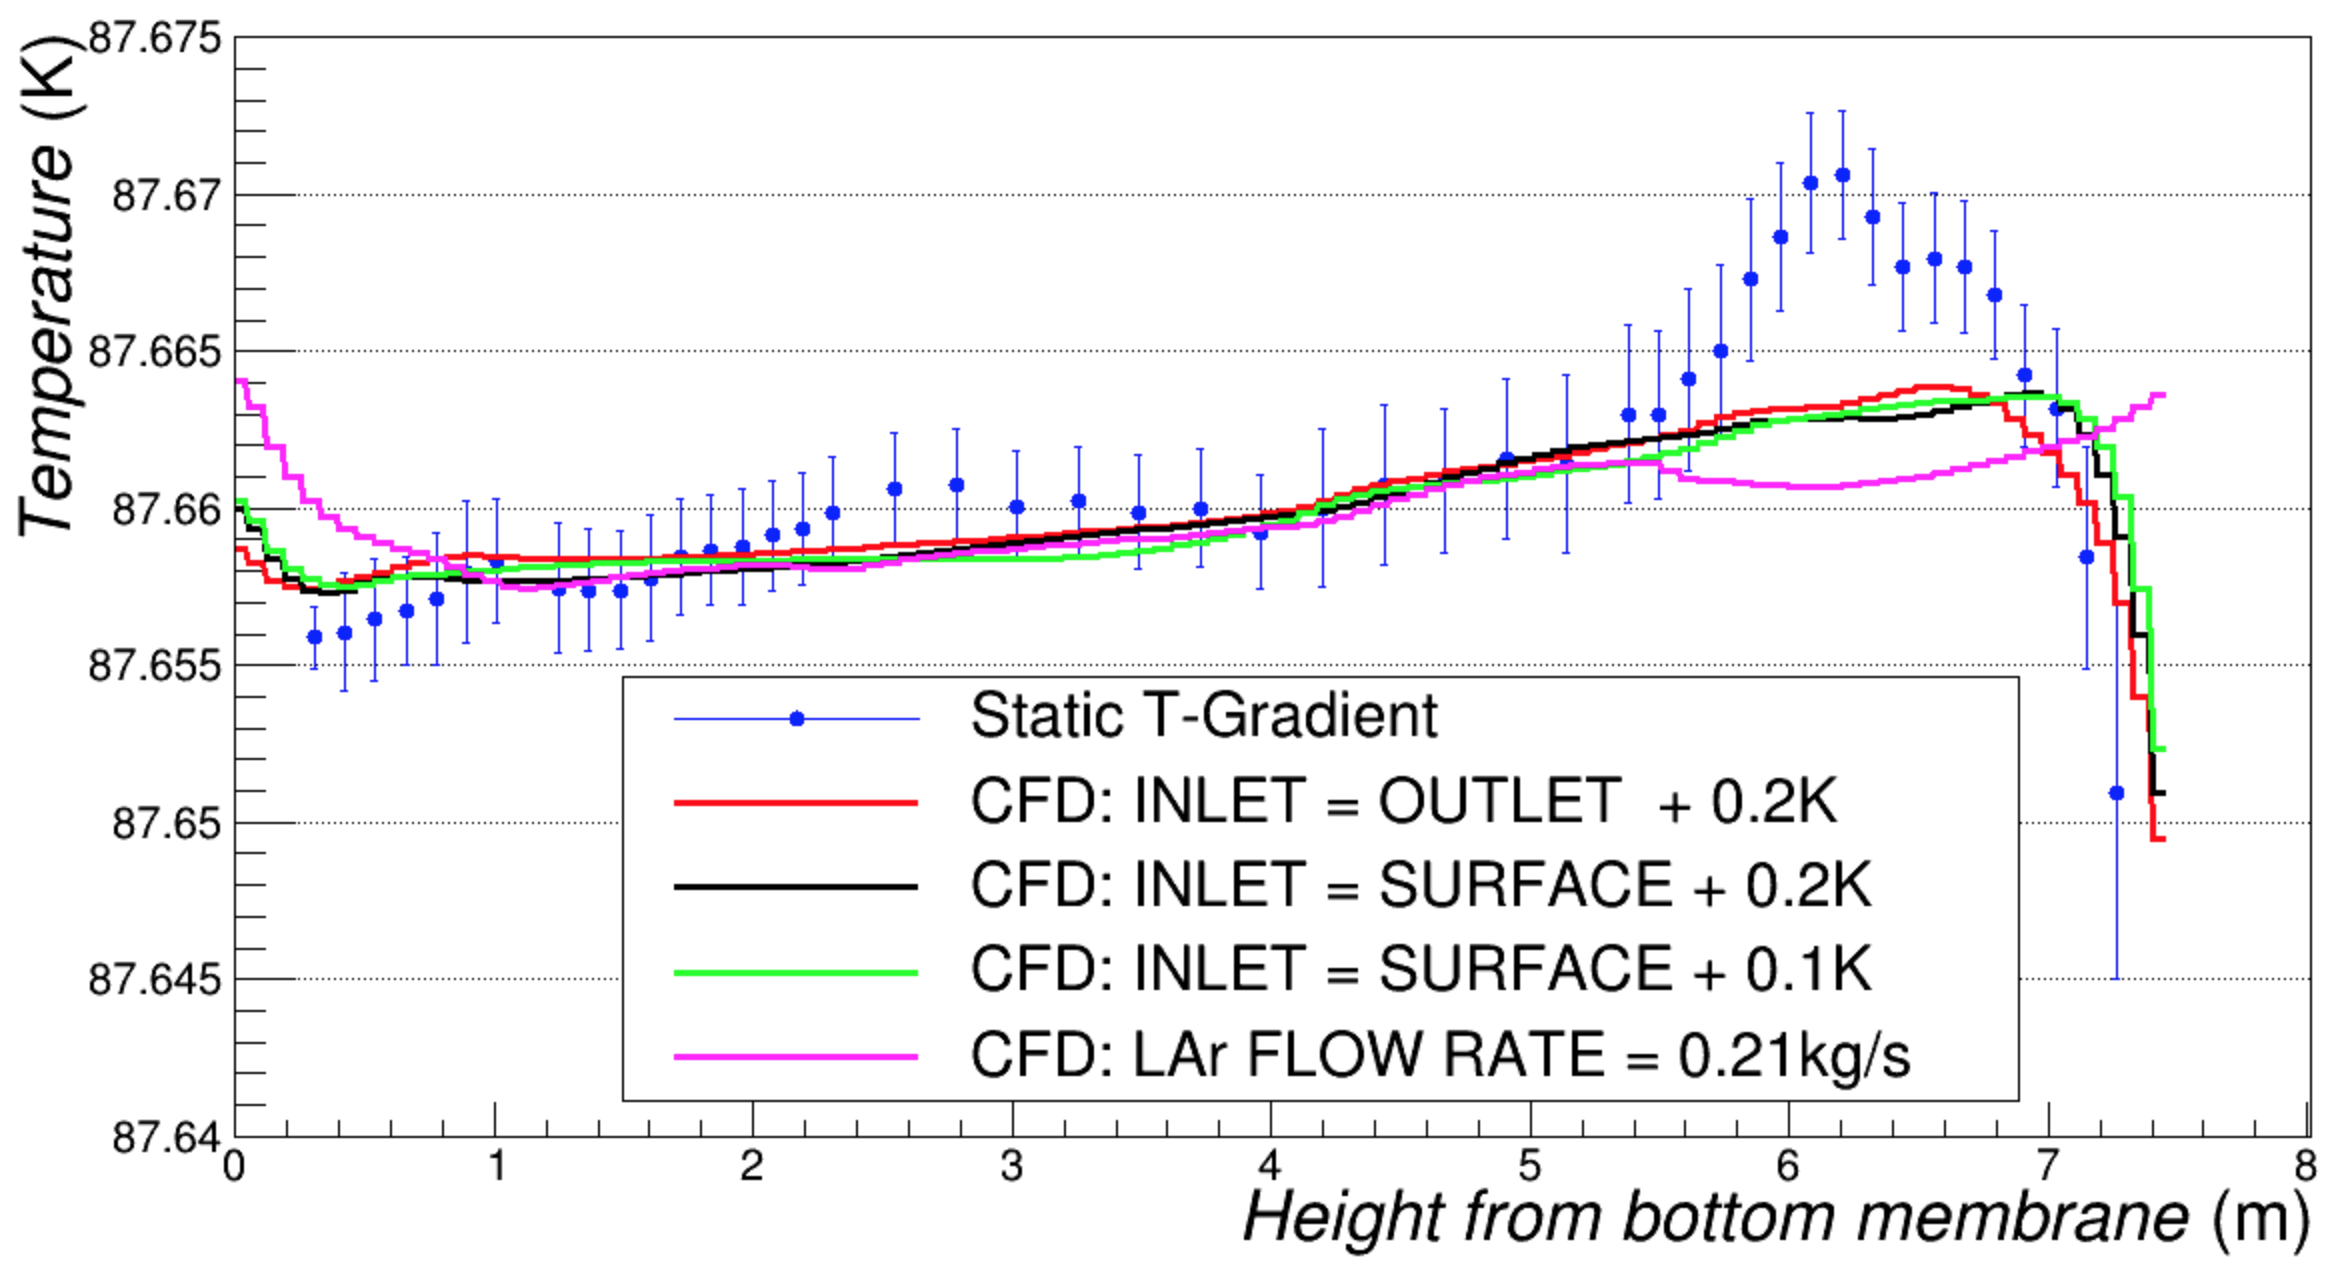
\includegraphics[width=0.5\textwidth]{cisc_static_cfd_data.png}%
\end{dunefigure}

In order to connect the two different %locations 
regions covered by the T-gradient monitors, temperature measurements by the bottom sensor grid can be used. Figure~\ref{fig:pd_t_bottom_results} shows the temperature difference between bottom sensors and the second sensor of the static T-gradient monitor (the one at 40~cm from the floor), which is used as reference. %It is also 
Also shown in the figure is the third sensor of the dynamic T-gradient monitor, located at a similar height. Three different periods are shown in the figure: two periods with pumps-on and one period with pumps-off. It is observed that when the pumps are working the temperature decreases towards the \dword{lar} pump, being  higher in the sensors below the cathode. The horizontal gradient observed in this situation is of the order of 20~mK -- larger than the vertical gradient. When the pumps are off the horizontal gradient decreases, although a residual gradient of 5 mk is observed. This gradient is attributed to the inertia of the liquid once the pumps are switched off: it takes more than one day to recover the horizontal homogeneity.    

\begin{dunefigure}[\dshort{pdsp} bottom sensor results ]{fig:pd_t_bottom_results}{Temperature difference between bottom sensors at 40~cm from the floor and static T-gradient sensor at same height. The third dynamic T-gradient sensor, which is  at the same height, is also shown. Two pumps-on periods (left and middle panels) and one pump-off period (right panel) are shown.}
  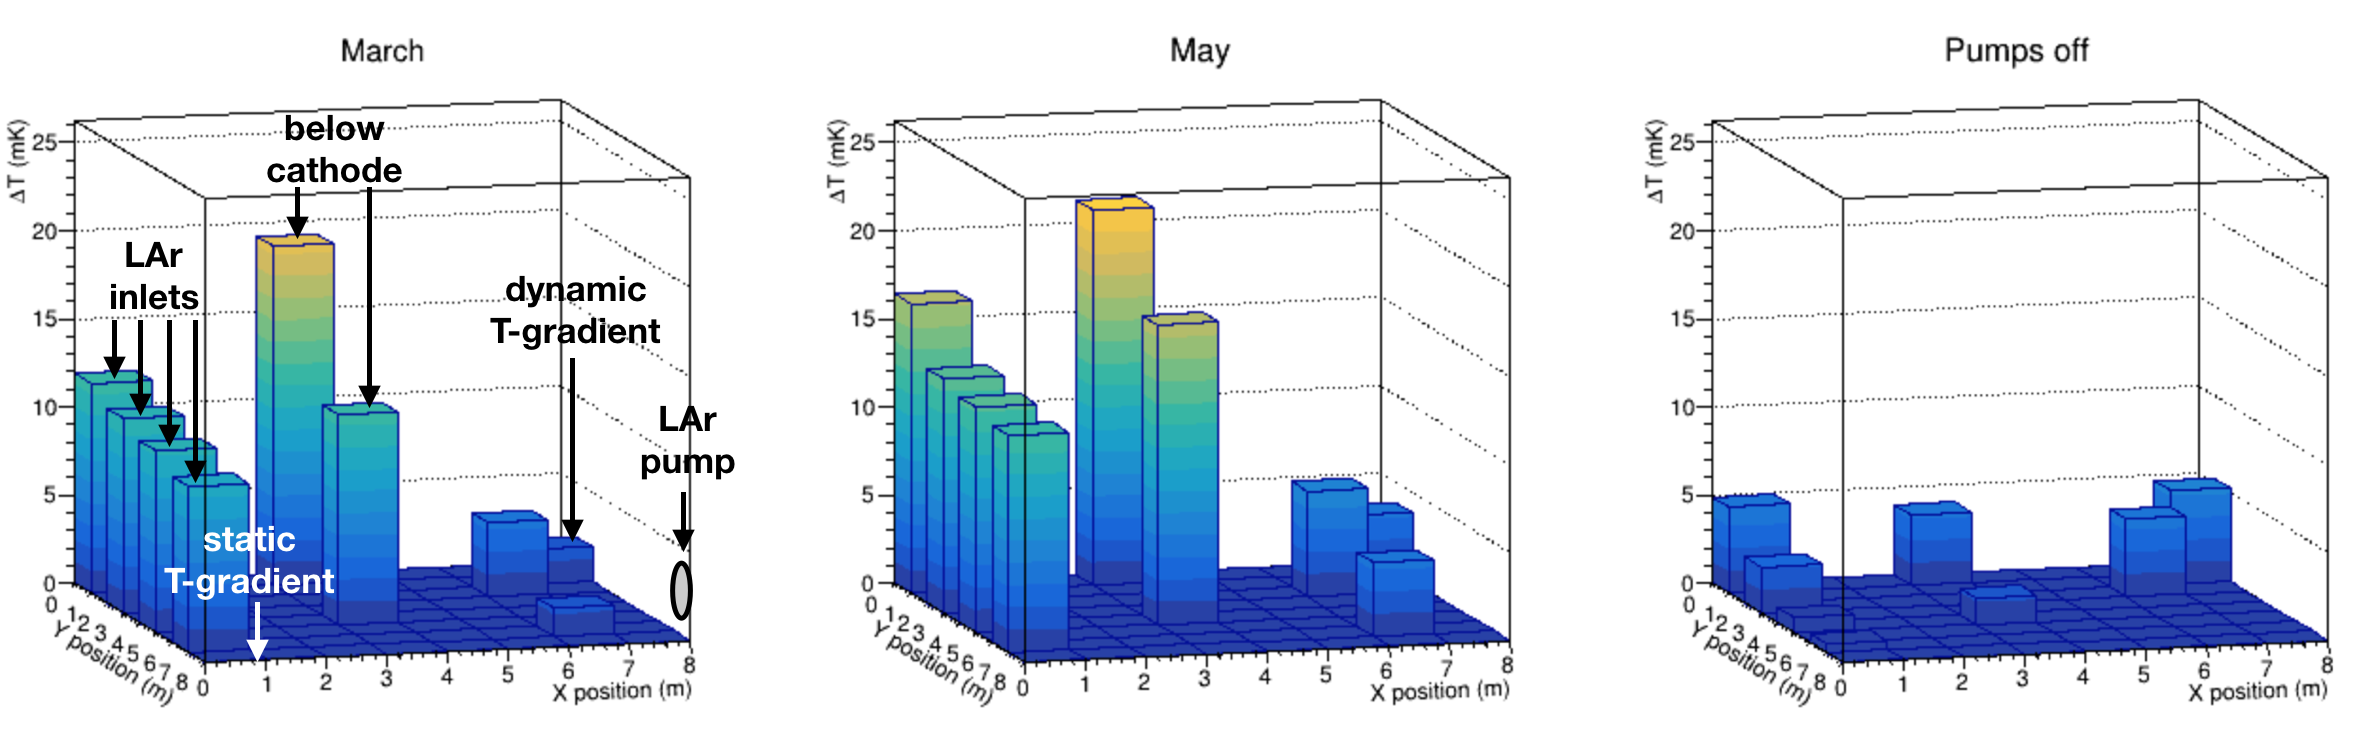
\includegraphics[width=0.95\textwidth]{cisc_t_bottom.png}%
\end{dunefigure}

\dword{cfd} simulations have been produced with different inputs. Two parameters have been identified as potential drivers of the convection regime: 1) the incoming \dword{lar} flow rate and 2) the incoming \dword{lar} temperature. The result of varying those parameters was shown in Figure~\ref{fig:pd_tgradient_results}. 
The \dword{cfd} model reasonably predicts the main features of the data but the details still need to be understood: the bump at 6.2~m or the lower measured temperature at the bottom. It is worth noting that the simulation depends minimally on the \dword{lar} temperature while the flow rate has more impact, specially in the regions where discrepancies are larger. All simulations use the nominal \dword{lar} flow rate, 0.42~kg/s, except the one explicitly indicated 
in the plots, which uses half of the rate. More simulations with other \dword{lar} flow rates are needed to conclude.  

The \dword{cfd} reassuringly predicts a reasonable response for more than one set of initial conditions. It is still important to %, but measure the 
instrumentation response to help establish the validity of the \dword{cfd} model. We did not run tests with differing initial conditions during the beam run because even controlled changes of the cryostat environment could have undesirable effects. However, dedicated tests to validate the \dword{cfd} under various deliberate changes of the cryostat were performed recently. Those  additional tests include pump and recirculation manipulations such as pump on-off, change of pumping speed, and bypassing of filtration, and changing the cryostat pressure set point to a higher (or lower) value\footnote{The \dword{hv} %could be 
was ramped down for this exercise because dropping the pressure too fast might provoke boiling of the \dword{lar} near the surface.} to induce changes in the pressure for a specified time while monitoring the instrumentation. Any change in pressure could change the temperatures everywhere in the cryostat. Studying the rate of this change, as detected at various heights in the cryostat, might provide interesting constraints on the \dword{cfd} model.

\subsubsubsection{Comparison of calibration methods}

Three different calibration methods have been described above, each of them having a different purpose. The underlying assumption is that reliable temperature monitoring at the few mK level is desirable during the entire lifetime of the experiment, both to guarantee the correct functioning of the cryogenics system and to compute offline corrections based on temperature measurements and \dword{cfd} simulations. This is only possible if an insitu calibration method is available since relative calibration between sensors is expected to diverge with time with respect to the one performed in the laboratory. Two insitu methods have been used. The pumps-off calibration method is very powerful since it is the only way of cross-calibrating all sensors in the cryostat at any point in time. However it relies on the assumption that the temperature is uniform when the recirculation pumps are off. The validity of this assumption has to be bench-marked with real data and this is done in \dword{pdsp} using the calibration based on the movable system (see Fig~\ref{fig:dynamic_t_pumps-off}). The last is the most precise calibration method and the one that sustains all other methods, providing a reliable reference during the entire lifetime of the experiment. This method is even more crucial for the far detector. Indeed, recirculation pumps will be located on one side of the cryostat, very far (almost \SI{60}{m}) from some regions of the \dword{lar} volume, where the inertia will be more pronounced and the homogeneous temperature assumption becomes less valid.   

% % % %
\subsubsection{Readout system for thermometers}
\label{sec:fdgen-slow-cryo-therm-readout}

A %highly precise 
high-precision and very stable system is required to achieve a readout level of $<\,\SI{5}{mK}$.
The proposed readout system was used in \dword{pdsp} and relies on a variant of an existing mass PT100 temperature readout system developed at
\dword{cern} for an \dword{lhc} 
experiment; it has already been tested and validated by the collaboration experts. The system has an electronic circuit that includes
\begin{itemize}
\item a precise and accurate current source for exciting the temperature sensors measured using the four-wires method;
\item a multiplexing circuit connecting the temperature sensor signals and forwarding the selected signal to a single line; and 
\item a readout system  with a high-accuracy voltage signal readout module\footnote{National Instrument CompactRIO\texttrademark{} device  with a signal readout NI9238\texttrademark{} module} with 24 bit resolution over a \SI{1}{V} range.
\end{itemize}
This readout system also drives the multiplexing circuit and calculates temperature values. The CompactRIO device is connected to the detector Ethernet network, sending temperature values to the \dword{dcs} software through a standard \dword{opc-ua} driver.


The current mode of operation averages more than \num{2000} samples taken every second for each sensor. 
Figure~\ref{fig:Trepro} shows the system has a resolution higher than 
\SI{1}{mK}, the \dword{rms} of one of the offsets in the stable region.


%%%%%%%%%%%%%%%%%%%%%%%%%%%%%%%%%%%%%%%%%%%%%%%%%%%%%%
%%%%%%%%%%%%%%%%%  PURITY MONITORS %%%%%%%%%%%%%%%%%%%

%%%%%%%%%%%%%%%%%%%%%%%%%%%%%%%%%%%

\subsection{Purity Monitors}
\label{sec:fdgen-slow-cryo-purity-mon}
%\fixme{CP: done, to be checked}
%Laura, Jianming
A fundamental requirement of a \dword{lar} \dshort{tpc} is that ionization electrons drift over long distances in \dword{lar}. Part of the charge is inevitably lost because of electronegative impurities in the liquid. To keep this loss to a minimum, monitoring impurities and purifying the \dword{lar} during operation is essential.


A purity monitor is a small ionization chamber used to infer independently  the effective free electron lifetime in the \dword{lartpc}.  
It illuminates a cathode with UV light to generate a known electron current, then collects the drifted current at an anode a known distance away.  Attenuation of the current is related to the electron lifetime.
Electron loss can be parameterized as
%
\(N(t) = N(0)e^{-t/\tau},\)
%
where $N(0)$ is the number of electrons generated by ionization, $N(t)$ is the number of electrons after drift time $t$, and $\tau$ is the electron lifetime. 

For the \dword{dpmod}, the drift distance is \dpmaxdrift, and the \efield is \SI{500}{\volt\per\centi\meter}. Given the drift velocity of approximately \SI{1.5}{\milli\meter\per\micro\second} in this field, the time to go from cathode to anode is roughly \SI{\sim8}{\milli\second} \cite{Walkowiak:2000wf}.
For a \dword{lartpc} signal attenuation, \([N(0)-N(t)]/N(0)\), of \SI{50}{\percent} over the entire drift distance,
 the corresponding electron lifetime is $\SI{8}{ms}/[-\ln(0.5)] \simeq \SI{11}{ms}$.

Residual gas analyzers can monitor the gas in the ullage of the tank and would be an obvious choice for analyzing argon gas. 
Unfortunately, suitable and commercially available mass
spectrometers have a detection limit of \SI{\sim 10}{\dword{ppb}},
whereas \dword{dune} requires a sensitivity of \dword{ppt}. Therefore,
specially constructed and distributed purity monitors will measure \lar purity in all %the
phases of operation. % at several known positions.  
These measurements,
along with an accurate \dword{cfd} model, enable 
determining \dword{lar} purity at all positions throughout the \dword{detmodule}.


Purity monitors also %serve to 
mitigate the risk of \lar contamination.  The large scale of the \dwords{detmodule} increases the risk of failing to notice a sudden, unexpected infusion of contaminated \lar %being injected 
back into the cryostat.   
If this condition were to persist, it could cause irreversible contamination to the \dword{lar} and terminate useful data taking.  Strategically placed purity monitors mitigate this risk as demonstrated in \dword{pdsp}. 

Purity monitors are placed inside the cryostat but outside the %detector 
\dword{tpc}. They are also placed  within the recirculation system outside the cryostat, both in front of and behind the filtration system. % before and after filtration. 
Continuous monitoring of  the \lar supply lines to the \dword{detmodule} provides a strong line of defense against %contaminated \lar. 
contamination from sources both in the \lar volume and from components in the recirculation system. 
Similarly, gas analyzers (described in Section~\ref{sec:fdgen-slow-cryo-gas-anlyz}) %provide a first line of defense 
protect against contaminated gas.  

Furthermore, using several purity monitors to measure lifetime with high precision at carefully chosen points provides key input, e.g.,  vertical gradients in impurity concentrations, for \dword{cfd} models of the \dword{detmodule}.

Purity monitors were deployed in previous \dword{lartpc} experiments, i.e., \dword{icarus}, \microboone, and the \dword{35t}. During the first run of the \dword{35t}, two of the four purity monitors stopped working during \cooldown, and a third operated intermittently. We later found this was due to poor electrical contacts between the resistor chain and the purity monitor. A new design was implemented and successfully tested in the second run. 



\dword{pdsp} and \dword{pddp} %use purity monitoring systems consisting of several 
implement purity monitors to %that 
measure electron lifetime at different heights.  
Both use a similar design. The baseline design for the \dword{dp} \dword{fd} will be the one used in \dword{pdsp}.
 
Figure~\ref{fig-pdsp-prmassembly} shows the assembly of the \dword{pdsp} purity monitors. The design reflects improvements to ensure electric connectivity and improve signals. \dword{pdsp} uses a string of purity monitors connected with stainless steel tubes to protect the optical fibers. The purity monitor system at \dword{pdsp} measured electron lifetime every hour during commissioning and daily during the beam test. During %commissioning and while running the test beam, 
this time, it %the purity monitor system at \dword{pdsp} 
alerted us to serious problems twice, first %. The first time was 
for filter saturation and %the second was 
then because the recirculation pump had stopped. This enabled us to prevent %These alerts were crucial to the success of running the test beam in the \dword{pdsp} project by preventing 
situations that otherwise could have had serious consequences.

\begin{dunefigure}[The \dshort{pdsp} purity monitoring system]{fig-pdsp-prmassembly}
  {The \dword{pdsp} purity monitoring system.}
  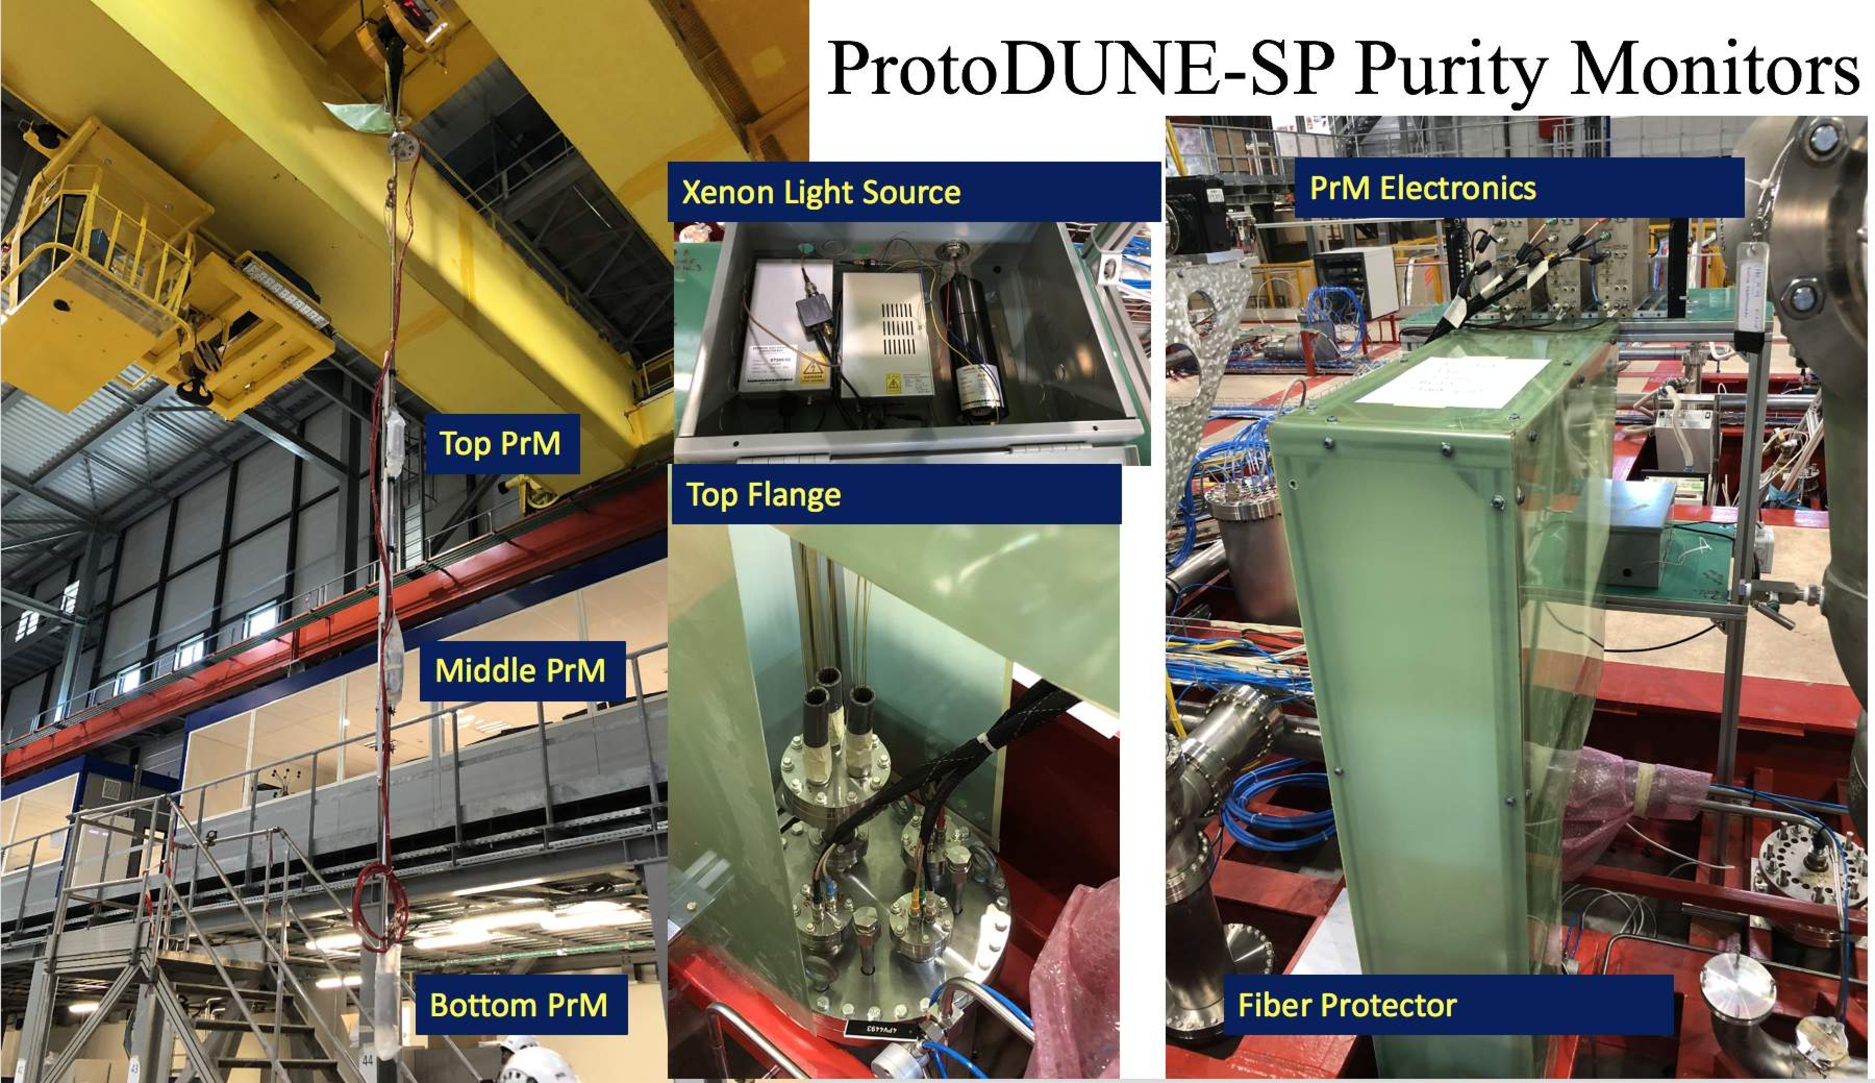
\includegraphics[width=0.9\textwidth]{PrMon_pdsp-PrMAssembly}
\end{dunefigure}



During the commissioning and beam test of \dword{pdsp}, the purity monitors operated with different high voltages to change electron drift time, ranging from \SI{150}{\micro\second} to \SI{3}{\milli\second}. This allowed the \dword{pdsp} purity monitors to measure electron lifetime from \SI{35}{\micro\second} to about \SI{10}{\milli\second} with high precision, a dynamic range greater than \num{300}. 
This measurement was also valuable for the \dword{pdsp} lifetime calibration. Because purity monitors have much smaller drift volumes than the \dword{tpc}, they are less affected by the space charge caused by cosmic rays. 

  A similar 
  %purity monitoring system design and 
  operation plan is foreseen for %are exploited in 
  the \dword{dpmod}, with modifications to accommodate the relative positions of the instrumentation port %placement relative to 
  and the purity monitor system and the %requirements and constraints of 
  different geometric relationships between the \dword{tpc} and cryostat.




%%%%%%%%%%%%%%%%%%%%%%%%%%%%%%%%%%%%%%%%%% 
%\subsubsection{Physics and Simulation}
% Andrew, Jianming


%\fixme{CP: Paragraph below modified.}
\dword{pdsp} implements three purity monitors instead of the two deployed in \dword{pddp}.
Figure~\ref{fig-pdsp-prm} shows the \dword{pdsp} data taken using %them 
its three purity monitors from commissioning of \dword{pdsp} starting in September 2018, through the entire beam running, to July 2019.

\begin{dunefigure}[Measured electron lifetimes in the %four 
three purity monitors at \dshort{pdsp}]{fig-pdsp-prm}
  {The electron lifetimes measured by three purity monitors in \dword{pdsp} as a function of time, September 2018 through July 2019. The purity is low prior to start of circulation in October. Reasons for later dips include recirculation studies and recirculation pump stoppages.}
  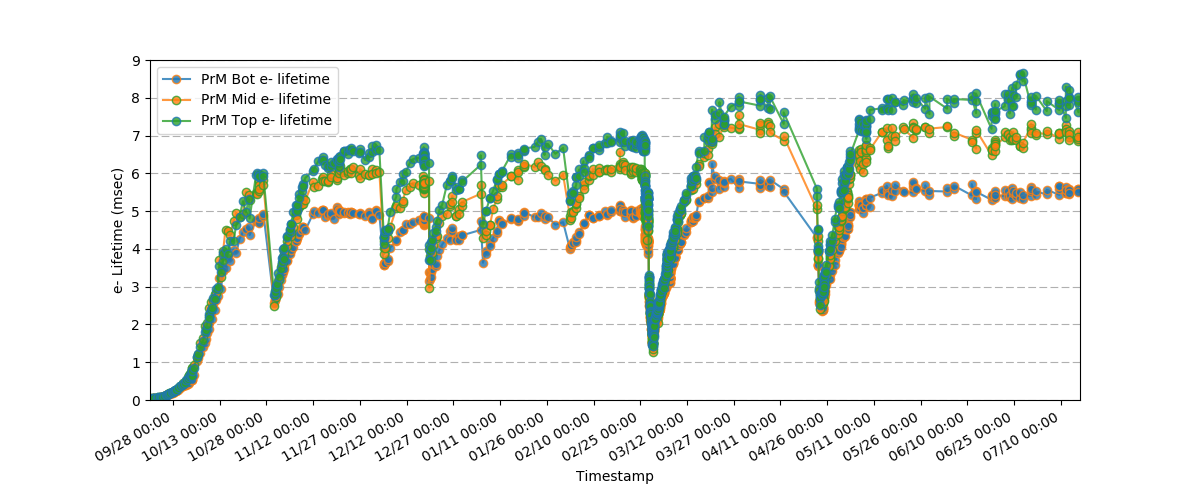
\includegraphics[width=0.9\textwidth]{cisc_pdsp_Lifetime_till_July17_without_error}
\end{dunefigure}

%%%%%%%%%%%%%%%%%%%%%%%%%%%%%%%%%%%%%%%%%
\subsubsection{Purity Monitor Design}

The \dword{dpmod} baseline purity monitor design follows that of  the \dword{icarus} experiment (Figure~\ref{fig:prm})\cite{Adamowski:2014daa}.  It consists of a double-gridded ion chamber immersed in the \lar volume with four parallel, circular electrodes, a disk holding a photocathode, two grid rings (anode and cathode), and an anode disk. The cathode grid is held at ground potential. The cathode, anode grid, and anode 
each hold separate bias voltages and are electrically accessible via modified vacuum-grade \dword{hv} \fdth{}s. % and separate bias voltages held at each one.   
The anode grid and the field-shaping rings are connected to the cathode grid by an internal chain of \SI{50}{\mega\ohm} resistors to ensure the uniformity of the \efield{}s in the drift regions. A stainless mesh cylinder is used as a Faraday cage to isolate the purity monitor from external electrostatic background. 

The purity monitor measures the electron drift lifetime between its anode and cathode. The purity monitor's UV-illuminated %gold 
photocathode generates electrons via the photoelectric effect. Because electron lifetime in \lar is inversely proportional to the electronegative impurity concentration, the fraction of electrons generated at the cathode that arrives at the anode ($Q_A/Q_C$) after the electron drift time $t$ gives a measure of the electron lifetime $\tau$:
%
\( Q_A/Q_C \sim e^{-t/\tau}.\)



\begin{dunefigure}[Schematic diagram of the %basic 
baseline purity monitor design]{fig:prm}
  {Schematic diagram of the basic purity monitor design \cite{Adamowski:2014daa}.}
  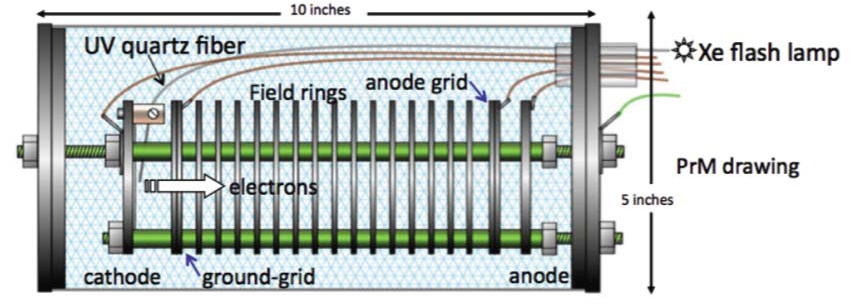
\includegraphics[width=0.9\textwidth]{PrMon_prm.pdf}
\end{dunefigure}



Once the electron lifetime becomes much larger than the drift time $t$, the purity monitor reaches its sensitivity limit.  For $\tau >> t$, the anode-to-cathode charge ratio becomes $\sim\,1$. Because the drift time is inversely proportional to the \efield, in principle, reducing the %drift 
field should make it possible to measure lifetimes of any length regardless of the length of the purity monitor.
On the other hand, increasing the voltage will shorten the drift time, allowing measurement of a short lifetime when purity is low. 


Varying the operational \dword{hv} on the anode from \SI{250}{V} to \SI{4000}{V} in the \dword{pdsp}'s \SI{24}{cm} (9.5 inch) long purity monitor allowed us to make the \SI{35}{\micro\second} to \SI{10}{\milli\second} electron lifetime measurements. 

The electron lifetime of the purest commercial \lar, after the first filtering and during the filling process, is typically longer than \SI{40}{\micro\second}. However, when the filter starts to saturate, the lifetime decreases to less than \SI{30}{\micro\second}.  To %achieve less 
reduce the energy loss due to impurities,  the \dword{dpmod} requires 
%an electron lifetime longer than \SI{10}{\milli\second}. 
at least \SI{3}{\milli\second} electron lifetime, with a goal of \SI{10}{\milli\second}. 
Therefore, purity monitors with different lengths (drift distances) are needed to extend the measurable range to less than \SI{35}{\micro\second} and more than  \SI{10}{\milli\second}.


The photocathode that produces the \phel{}s is an aluminum plate coated first with \SI{50}{\angstrom} of titanium followed by \SI{1000}{\angstrom} of gold; it is attached to the cathode disk.
Three photocathodes per purity monitor are implemented in \dword{pddp}, two of silver and one of gold, with each cathode lit by one fiber. The gold cathode is the standard used in \dword{pdsp}, but R\&D has shown silver emits more photoelectrons.
A xenon flash lamp is the light source in the baseline design, although %this could be replaced by 
a more reliable and possibly submersible light source, perhaps \dword{led}-driven, could replace this in the future. The UV output of the lamp is quite good, approximately $\lambda=$ \SI{225}{\nano\meter}, which corresponds closely to the work function of gold (\SIrange{4.9}{5.1}{\eV}). 
%Several 
Three UV quartz fibers carry the xenon UV light into the cryostat to illuminate the %gold 
photocathode.   Another quartz fiber delivers the light into a properly biased photodiode outside the cryostat to provide the trigger signal when the lamp flashes. 



\subsubsection{Electronics, DAQ, and Slow Controls Interfacing}
%Jianming
The purity monitor electronics and \dword{daq} system consist of \dword{fe} electronics, waveform digitizers, and a \dword{daq} PC.  Figure~\ref{fig:cryo-purity-mon-diag} %shows the block diagram of the 
illustrates the system.

\begin{dunefigure}[Block diagram of the purity monitor system]{fig:cryo-purity-mon-diag}
  {Block diagram of the purity monitor system.}
  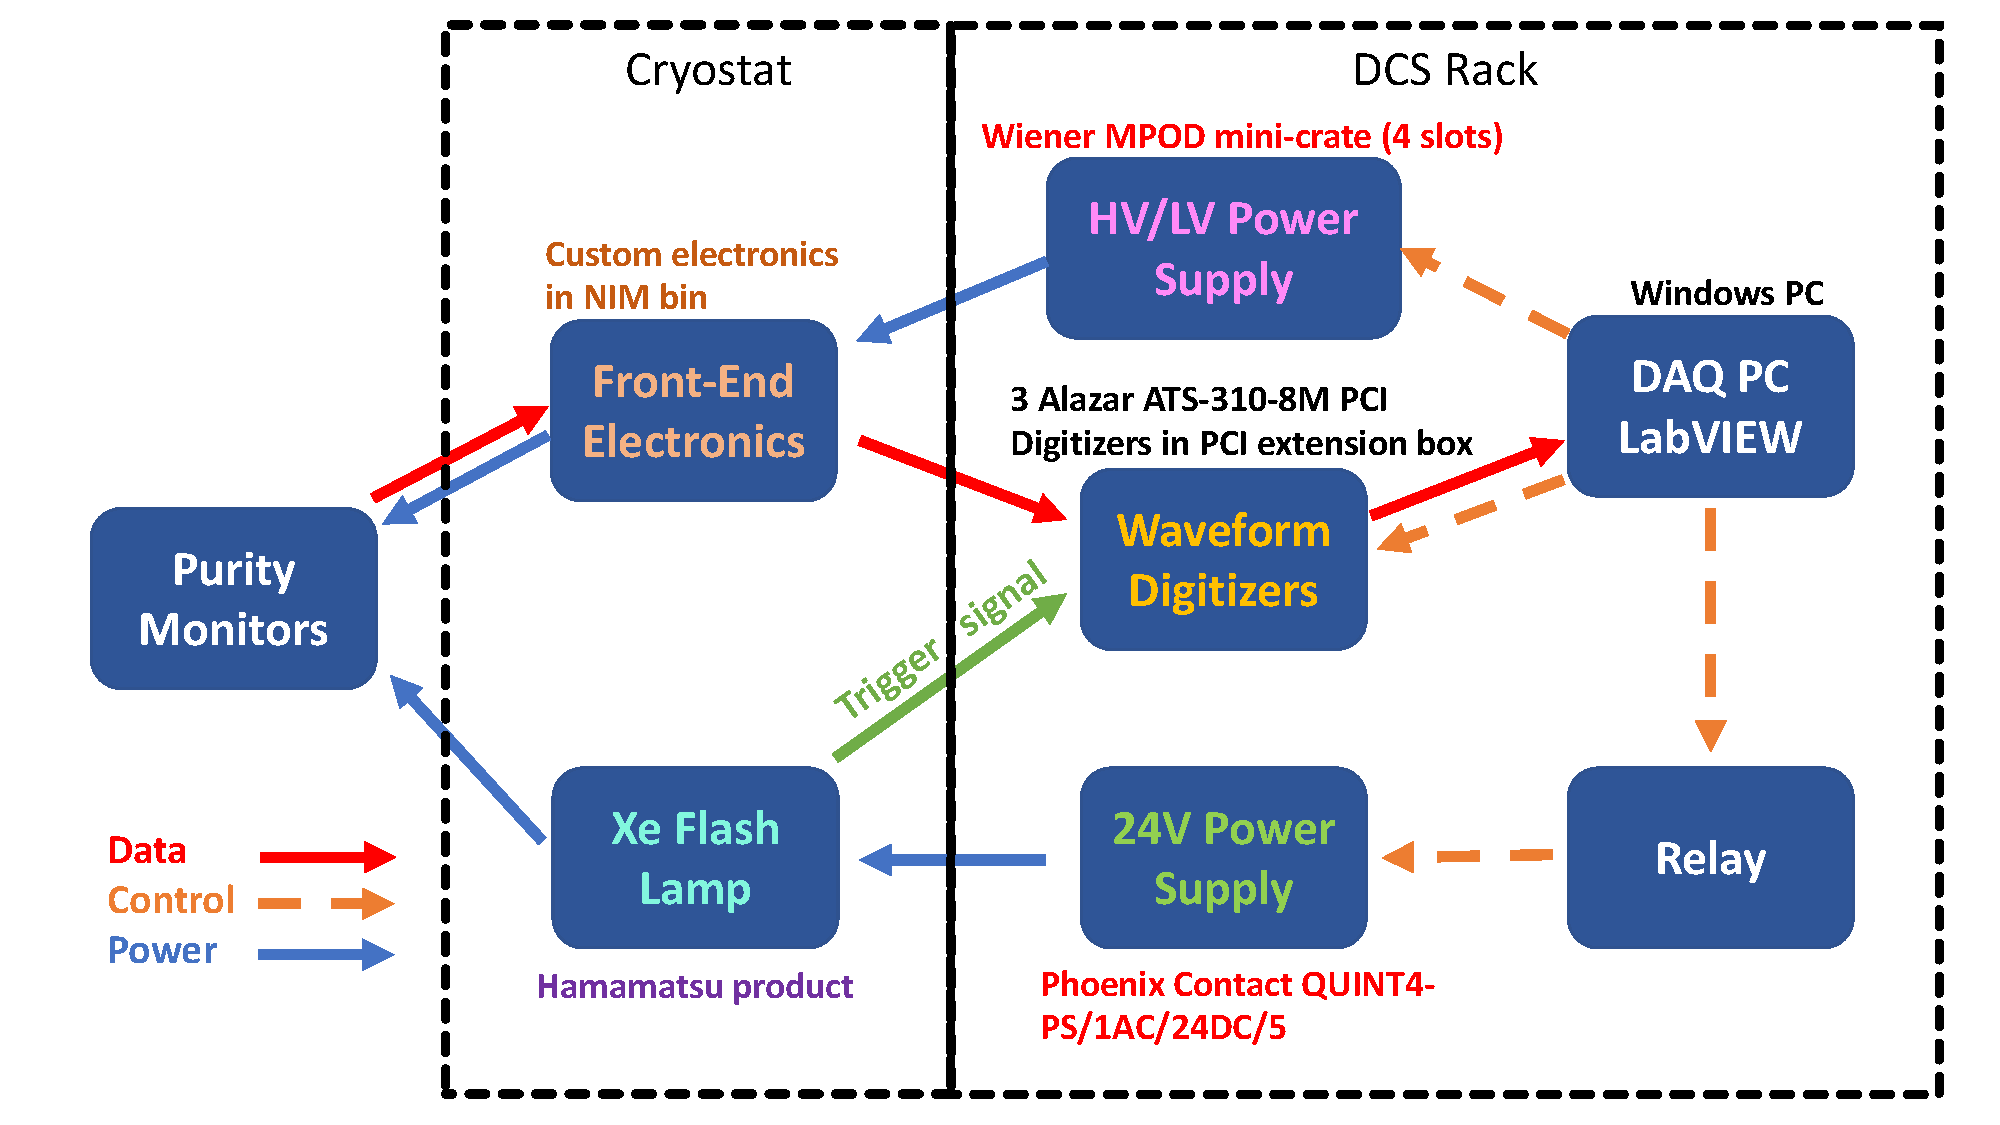
\includegraphics[width=0.95\textwidth]{graphics/PrMon_BlockDiagram_v2.pdf}
\end{dunefigure}


The baseline design of the \dword{fe} electronics follows the one used in %is the one used for the purity monitors for 
the \dword{35t}, \dword{lapd}, 
and \microboone. The cathode and anode signals are fed into two charge amplifiers within the purity monitor electronics module.
This electronics module includes a \dword{hv} filter circuit and an amplifier circuit, both shielded by copper plates, to allow the signal and \dword{hv} to be carried on the same cable and decoupled inside the purity monitor electronics module. 
A waveform digitizer that interfaces with a \dword{daq} PC records the amplified anode and cathode outputs. 
The signal and \dword{hv} cable shields connect to the grounding points of the cryostat and are separated from the electronic ground with a resistor and a capacitor connected in parallel and mitigating ground loops between the cryostat and the electronics racks. Amplified output is transmitted to an AlazarTech ATS310 waveform digitizer\footnote{AlazarTech ATS310\texttrademark{} - 12 bit, 20 MS/s,  https://www.alazartech.com/Product/ATS310.} containing two input channels, each with 12 bit resolution. Each channel can sample a signal at a rate of \SI{20}{\mega\samples\per\second} to \SI{1}{\kilo\samples\per\second} and store up to \SI{8}{\mega\samples} in memory. One digitizer is used for each purity monitor, and each digitizer interfaces with the \dword{daq} PC across the \dword{pci} bus. 
%\fixme{add PCI and labview to glossary? anne}

A custom \dword{labview}\footnote{National Instruments, LabVIEW\texttrademark{}, http://www.ni.com/en-us.html} application running on the \dword{daq} PC has two functions: it controls the waveform digitizers and the power supplies, and it monitors the signals and key parameters. The application configures the digitizers to set the sampling rate, the number of waveforms to be stored in memory, the pre-trigger data, and a trigger mode. A signal from a photodiode triggered by the xenon flash lamp is fed directly into the digitizer as an external trigger to initiate data acquisition.  \dword{labview} automatically turns on the xenon flash lamp by powering a relay when data taking begins and then turning it off when finished.
The waveforms stored in the digitizers are transferred to the \dword{daq} PC and used to obtain averaged waveforms to reduce any electronic noise in them. % waveforms. 

The baseline  is estimated by averaging the waveform samples prior to the trigger. This baseline is subtracted from the waveforms prior to calculating peak voltages of the cathode and anode signals. %These processes are performed in real time within the application and are then used to estimate the electron lifetime.
The application performs these processes in real time. % within and uses the results to estimate the electron lifetime. 
 The application continuously displays the waveforms and important parameters like measured electron lifetime, peak voltages, and drift time % of electrons 
in the purity monitors and shows the variation in these parameters over time, thus pointing out %.This allows validating the impurity of the \dword{lar} and seeing 
effects that might otherwise be missed. %may not be spotted at that instant. 
Instead of storing the measured parameters, the waveforms and the digitizer configurations are recorded in binary form for offline analysis.  \dword{hv} modules\footnote{iseg Spezialelektronik GmbH\texttrademark{} high voltage supply systems, https://iseg-hv.com/en.} in a WIENER MPOD mini crate\footnote{W-IE-NE-R MPOD\texttrademark{} Universal Low and High Voltage Power Supply System, \url{http://www.wiener-d.com/}.} supply negative voltages to the cathode and positive voltages to the anode. The \dword{labview} application controls and monitors the \dword{hv} systems through an Ethernet interface.


The xenon flash lamp and the \dword{fe} electronics are installed close to the purity monitor flange to reduce light loss through the optical fiber and prevent signal loss. Other pieces of equipment that distribute power to these items and collect data from the electronics are mounted in a rack separate from the cryostat. The slow control system communicates with the purity monitor \dword{daq} software and controls  the \dword{hv} and \dword{lv} power supplies of the purity monitor system. The optical fiber must be placed within  \SI{0.5}{\milli\meter} of the photocathode for efficient \phel extraction, so little interference with the \dword{pds} is expected. The purity monitors could induce noise in the \dword{tpc} electronics, in particular via the current surge through a xenon lamp when it is flashed.  This source of noise can be controlled by placing the lamp inside its own Faraday cage with %, which allows 
proper grounding and shielding. %According to the operation of purity monitors 
At \dword{pdsp}, after careful checks of the grounding, this noise has remained well below the noise generated by other sources.

In the \dword{dpmod} we can make use of triggering to prevent any potential noise from the purity monitor's flash lamp from affecting \dword{tpc} and \dword{pds} signals. The \dword{lartpc} trigger rate is a few hertz, and each trigger window is one or a few milliseconds. %For a purity monitor's flash lamp,  the flash light 
The pulse from a flash lamp is very short (a microsecond or so, much shorter than the gaps between \dword{lartpc} trigger windows). 
Thus, an \dword{lartpc} trigger signal may be sent to a programmable pulse generator, %and the pulse generator then 
which generates a trigger pulse that does not overlap with \dword{lartpc} trigger windows. This trigger pulse %will then be 
is then sent to the external trigger port on the flash lamp \dword{hv} controller, so the lamp flashes between \dword{lartpc} trigger windows. In this way, the electronic and light noises from the flash lamp do %will 
not affect %LArTPC 
data taking at all.


%%%%%%%%%%%%%%%%%%%%%%%%%%%%%%%%%%%%%%%%%%
\subsubsection{Production and Assembly}
\label{sec:PrMon-Production-Assembly}

The \dword{cisc} consortium will produce the individual purity monitors, test them in a test stand, and confirm that each monitor operates at the required level before assembling them into strings of three monitors that will be mounted in the \dword{dpmod} cryostat using support tubes. The assembly process will follow the methodology developed for \dword{protodune}.



A short version of the %assembly
string
%\fixme{string?}
with all purity monitors will be tested at the \dword{citf}. 
%in the \lar test facility. 
The full string will be assembled and shipped to  \dword{surf}. 
 A vacuum test in a long vacuum tube will be performed on site before inserting the full assembly into the \dword{dpmod} cryostat. 


%%%%%%%%%%%%%%%%%%%% LIQUID LEVEL MONITORING %%%%%%%%%%%%%%%%%%%%
\subsection{Liquid Level Meters}
% john L, anselmo
% SP

%\fixme{SG/ACV: Done. To be checked !!!!}

The goals for the \dword{lar} level monitoring system are basic level sensing when filling, and precise level sensing during static operations.  The system also provides signals for \dword{ddss} interlocks that protect the detector (e.g.,\ \dword{hv}). \dword{dune} will use both differential pressure level meters (\dword{lbnf} scope) and capacitive level meters (\dword{dune} scope). Liquid level meters provide useful information for both cryostat filling and stable operation. Dedicated level meters will be complemented by vertical arrays of temperature sensors (see Section~\ref{sec:fddp-cryo-therm}), located at known heights and used to determine the \lar level (they will change temperature dramatically when the cold liquid reaches each of them), and by cameras, which will focus on the \lar surface at all times.  \fixme{all but first sentence of prev pgraph not in sp; ok?}

Filling the cryostat with \lar will take several months. During this operation, several systems will monitor the \lar level. 
The first \SI{5.5}{m} of \dword{lar} will be monitored by cameras and by the vertical arrays of \dwords{rtd}. Once the liquid reaches the level of the cryogenic pipes going out of the cryostat, 
the differential pressure between that point and the bottom of the cryostat
can be converted to depth using
the known density of \lar.  Fine tuning the final \dword{lar} level require several capacitive level meters at the top of the cryostat; this system comprises several \SI{4}{m}  long capacitive level sensors (with a precision of less than \SI{5}{mm} ) which will be checked against each other. One capacitive level sensor at each of the four corners of the cryostat will provide sufficient redundancy to ensure that no single point of failure compromises the %capacitive level sensor 
measurement.


During operations, liquid level monitoring has two purposes:
monitoring to tune the \lar flow, and monitoring for safety interlocking purposes and for cross checks. 


The \lar flow is tuned using two differential pressure level meters, installed as part of the cryogenics system, one on each side of the \dword{detmodule}.  They have a precision of \SI{0.1}{\%}, which corresponds to \SI{14}{mm} at the nominal \dword{lar} surface. Cryogenic pressure sensors will be purchased from commercial sources. Installation methods and positions will be determined as part of the cryogenic internal piping plan. 
The dual phase technology must control the \dword{lar} surface at the sub-millimeter level, so fine tuning the \dword{lar} level will require two high-precision capacitive level meters attached to the inner cryostat membrane at the appropriate height.   


For %\dword{hv} integrity
safety interlocking and to cross check measurements with differential pressure level meters the long capacitive level meters will be used. 


In addition to these level meters, \dword{crp} will use high precision (less than \SI{1}{mm}) capacitive level meters attached to the \dword{crp} frame to monitor constant \dword{crp} alignment to the liquid phase. These fall under the scope of the \dword{crp} consortium and are described in Chapter~\ref{ch:dp-crp} of this \dword{tdr} volume.

Figure~\ref{fig:cisc_pdsp_level} shows the evolution of the \dword{pdsp} \dword{lar} level over two months as measured by the differential pressure and capacitive level meters. 

\begin{dunefigure}[\lar level measurements]{fig:cisc_pdsp_level}{Evolution of the \dword{pdsp} \lar level over two months. Left: Measured by the capacitive level meter. Right: Measured by the differential pressure level meter. The units in the vertical axis are percentages of the cryostat height (\SI{7878}{mm}).}
  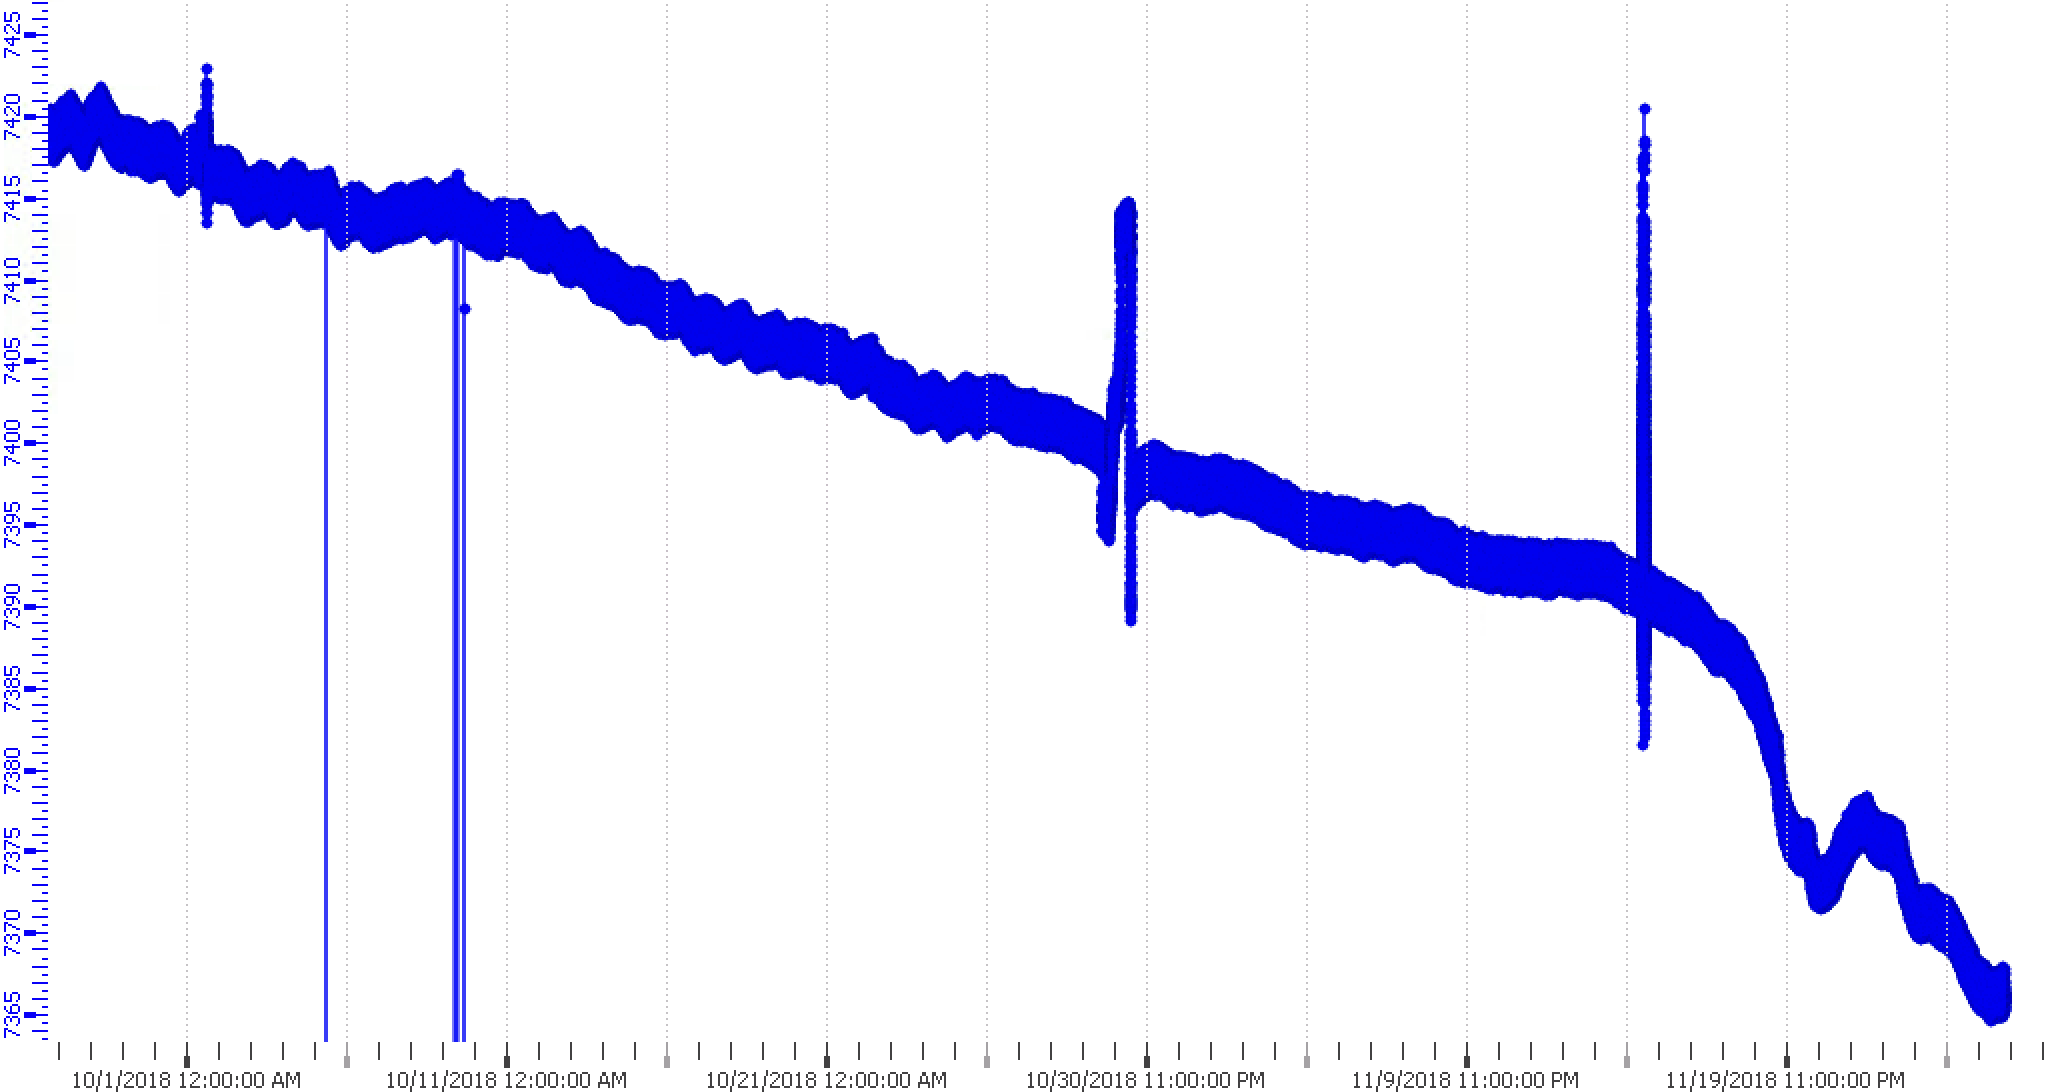
\includegraphics[width=0.45\textwidth]{cisc_level_cap.png}%
  \hspace*{1cm}
  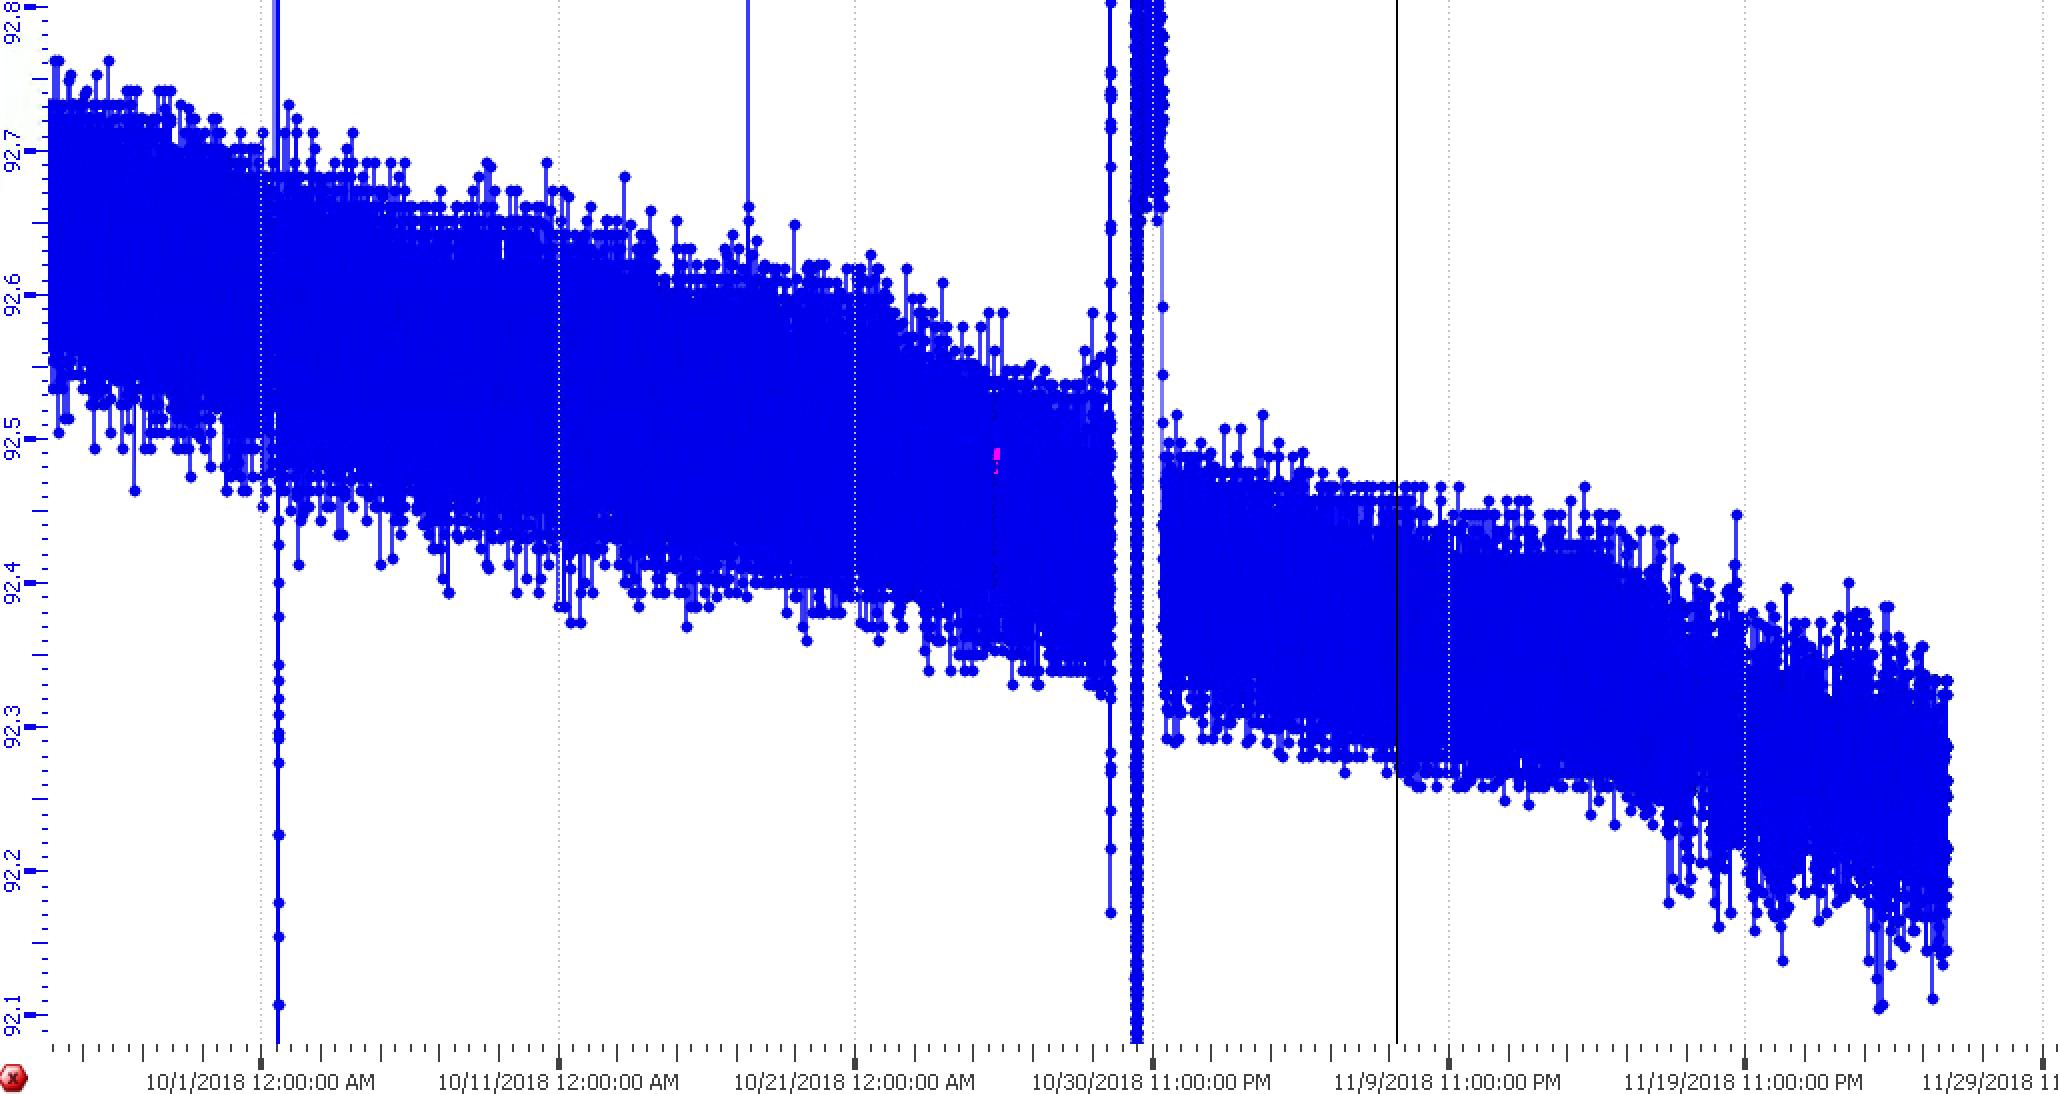
\includegraphics[width=0.45\textwidth]{cisc_level_diffp.png}%
\end{dunefigure}

\dword{pdsp} and \dword{pddp} use the same design for differential pressure level meters; this design  will also be used in the far detector \dword{sp} and \dword{dp} modules. For the capacitive level meters, \dword{pdsp} is using commercial  \SI{1.5}{m} long level meters while \dword{pddp} is using \SI{4}{m} long level meters custom-built by \dword{cern}. For the \dword{dune} \dword{fd}, we plan to use the longer capacitive level meters custom-built by \dword{cern} for both \dword{sp} and \dword{dp} modules.



\subsection{Pressure Meters}
\label{sec:fdgen-slow-cryo-press-meter}

%\fixme{SG/ACV:Done. New section for DP only}

Measuring the pressure of argon gas in the DUNE \dword{fd} is important because it can affect gas density, and consequently, the \dword{lem} gain calibration. The accuracy of the pressure sensors should be within at least 0.1\% or more of the real value. %The pressure needs to be monitored to 1~mbar precision and accuracy. 
Moreover, the absolute temperature in the liquid varies with the pressure in the argon gas, so precise measurements of pressure inside the cryostat provides a better picture of temperature gradients and \dword{cfd} simulations. In \dword{protodune}, pressure values were also used to understand the strain gauge signals installed in the cryostat frame.

Standard industrial pressure sensors can be used for this. For the \dword{dune} \dword{fd}, the plan is to follow the same design and configuration used in \dword{pdsp} and \dword{pddp}. \dword{protodune} uses two types of pressure sensors and a pressure switch, % as described below:
\begin{itemize}
    \item a relative pressure sensor (range: 0-400~mbar, precision: 0.01~mbar),
    \item an absolute pressure sensor (range: 0-1600~mbar, precision: 0.05~mbar), and
    \item a mechanical relative pressure switch adjustable from 50 to 250~mbar. 
\end{itemize}


Both sensors and the pressure switch are installed in a dedicated flange as shown in Figure~\ref{fig:pdsp-pressure} and are connected directly to a slow controls system \dword{plc} circuit. Dedicated analogue inputs are used to read the current values (\SIrange{4}{20}{mA}), which are then converted to pressure according to sensor range. Given the much larger size of the \dword{dune} \dwords{detmodule}, this system will be doubled for redundancy: two flanges in opposite cryostat sides will be instrumented with three sensors each. 

\begin{dunefigure}[Photo of the pressure sensors installed on a flange in ProtoDUNE-SP]{fig:pdsp-pressure}
  {Photograph of the pressure sensors installed on a flange in \dword{pdsp}.}
  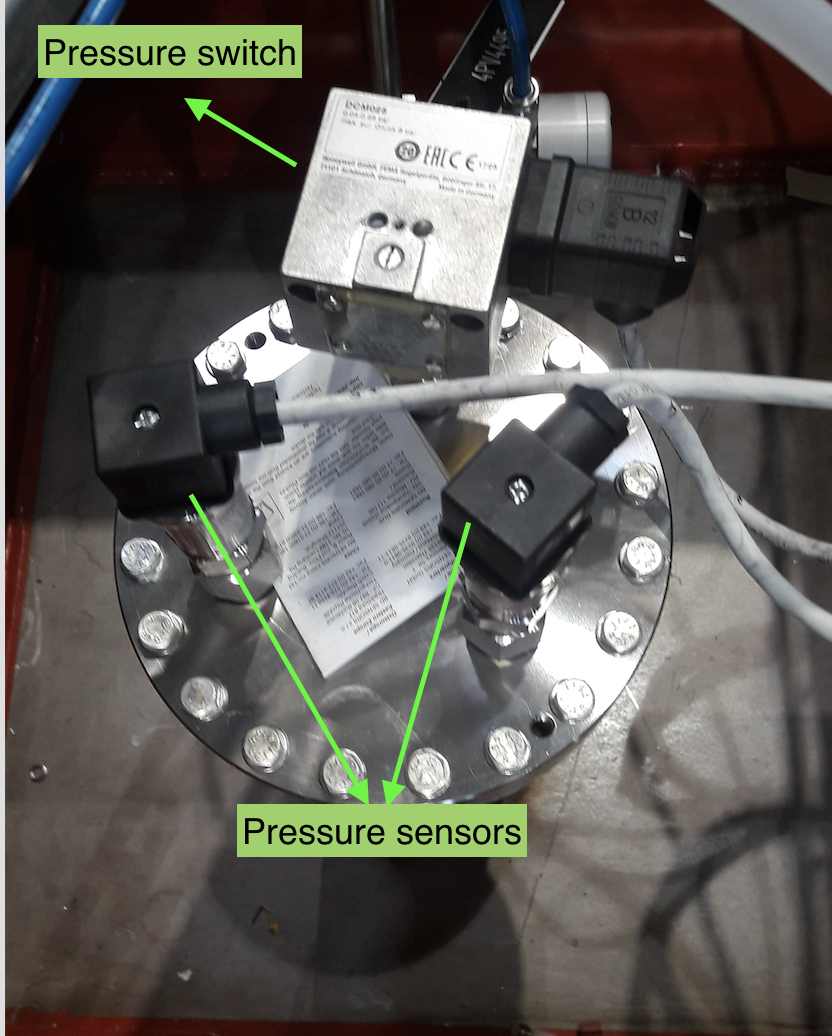
\includegraphics[width=0.5\textwidth]{graphics/cisc-pdsp-pressure-meters}
\end{dunefigure}

Further, relative and absolute pressure sensors (with comparatively lower precision) are installed by \dword{lbnf} that are also recorded by the slow controls system. The availability of two types of sensors from \dword{lbnf} and \dword{cisc} provides redundancy, independent measurements, and cross checks.

%%%%%%%%%%%%%%%%%%% GAS ANALYZERS %%%%%%%%%%%%%%%%%%%%
\subsection{Gas Analyzers}
\label{sec:fdgen-slow-cryo-gas-anlyz}
% alan h
%\fixme{CP: Valid Section; Alan checked and made small edits}
 Gas analyzers are commercially produced modules that measure trace quantities of specific gases contained within a stream of carrier gas. The carrier gas for \dword{dune} is argon, and the trace gases of interest are oxygen ($\text{O}_2$), water ($\text{H}_2\text{O}$), and nitrogen ($\text{N}_2$). $\text{O}_2$ and $\text{H}_2\text{O}$ affect the electron lifetime in \dword{lar} and must be kept below \SI{0.1}{ppb} ($\text{O}_2$ equivalent) while $\text{N}_2$ affects the efficiency of scintillation light production at levels higher than \SI{1}{ppm}.
The argon is sampled from either the argon vapor in the ullage or from the \dword{lar} by using small diameter tubing run from the sampling point to the gas analyzer. Typically, the tubing from the sampling points are connected to a switchyard valve assembly used to route the sample points to the desired gas analyzers (see Figure~\ref{fig:GA-switchyard}).


\begin{dunefigure}[Photo of a gas analyzer switchyard valve assembly]{fig:GA-switchyard}
  {A gas analyzer switchyard that routes sample points to the different gas analyzers.}
  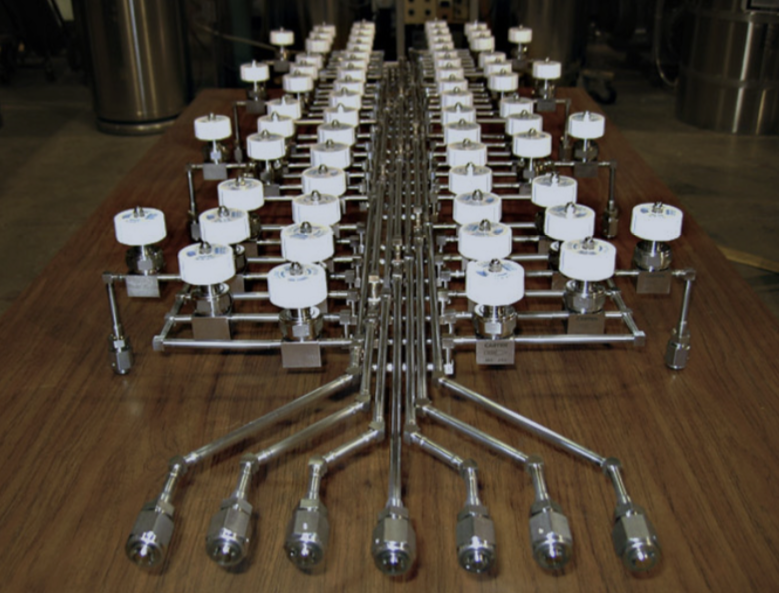
\includegraphics[width=0.9\textwidth]{cisc_GasAnalyzerSwitchyard.png}
\end{dunefigure}

%The following lists three times 
The gas analyzer would be predominantly used during three periods: 


\begin{enumerate}
\item Once the detector is installed and after the air atmosphere is eliminated from the cryostat to levels low enough to begin \cooldown. This purge and gas recirculation process is detailed in Section~\ref{sec:fdgen-slow-cryo-install-ga}. Figure~\ref{fig:cisc_Phase1_purge_gas_recirculation} shows the evolution of the $\text{N}_2$, $\text{O}_2$, and $\text{H}_2\text{O}$ levels from gas analyzer data taken during the purge and recirculation stages of the \dword{dune} \dword{35t} %Prototype P
phase 1 run.


\item Before other means of monitoring impurity levels (e.g., purity monitors or \dshort{tpc} tracks) are sensitive, to track trace $\text{O}_2$ and $\text{H}_2\text{O}$ contaminants from $\>$tens of ppb to hundreds of ppt.  Figure~\ref{fig:cisc_O2AnalyzerPrM2_HVRun1} shows an example plot of $\text{O}_2$ levels at the beginning of \lar purification from one of the later \dword{35t} \dword{hv} runs.

\item During cryostat filling to monitor the tanker \lar delivery purity. This tracks the impurity load on the filtration system and rejects any deliveries that do not meet specifications. Likely specifications for delivered \lar are in the \SI{10}{ppm} range per contaminant.


\end{enumerate}

\begin{dunefigure}[Impurity levels during the pre-fill stages for the \SI{35}{t} phase 1]{fig:cisc_Phase1_purge_gas_recirculation}
  {Plot of the $\text{O}_2$, $\text{H}_2\text{O}$, and $\text{N}_2$ levels during the piston purge and gas recirculation stages of the \dword{35t} Phase 1 run.}
  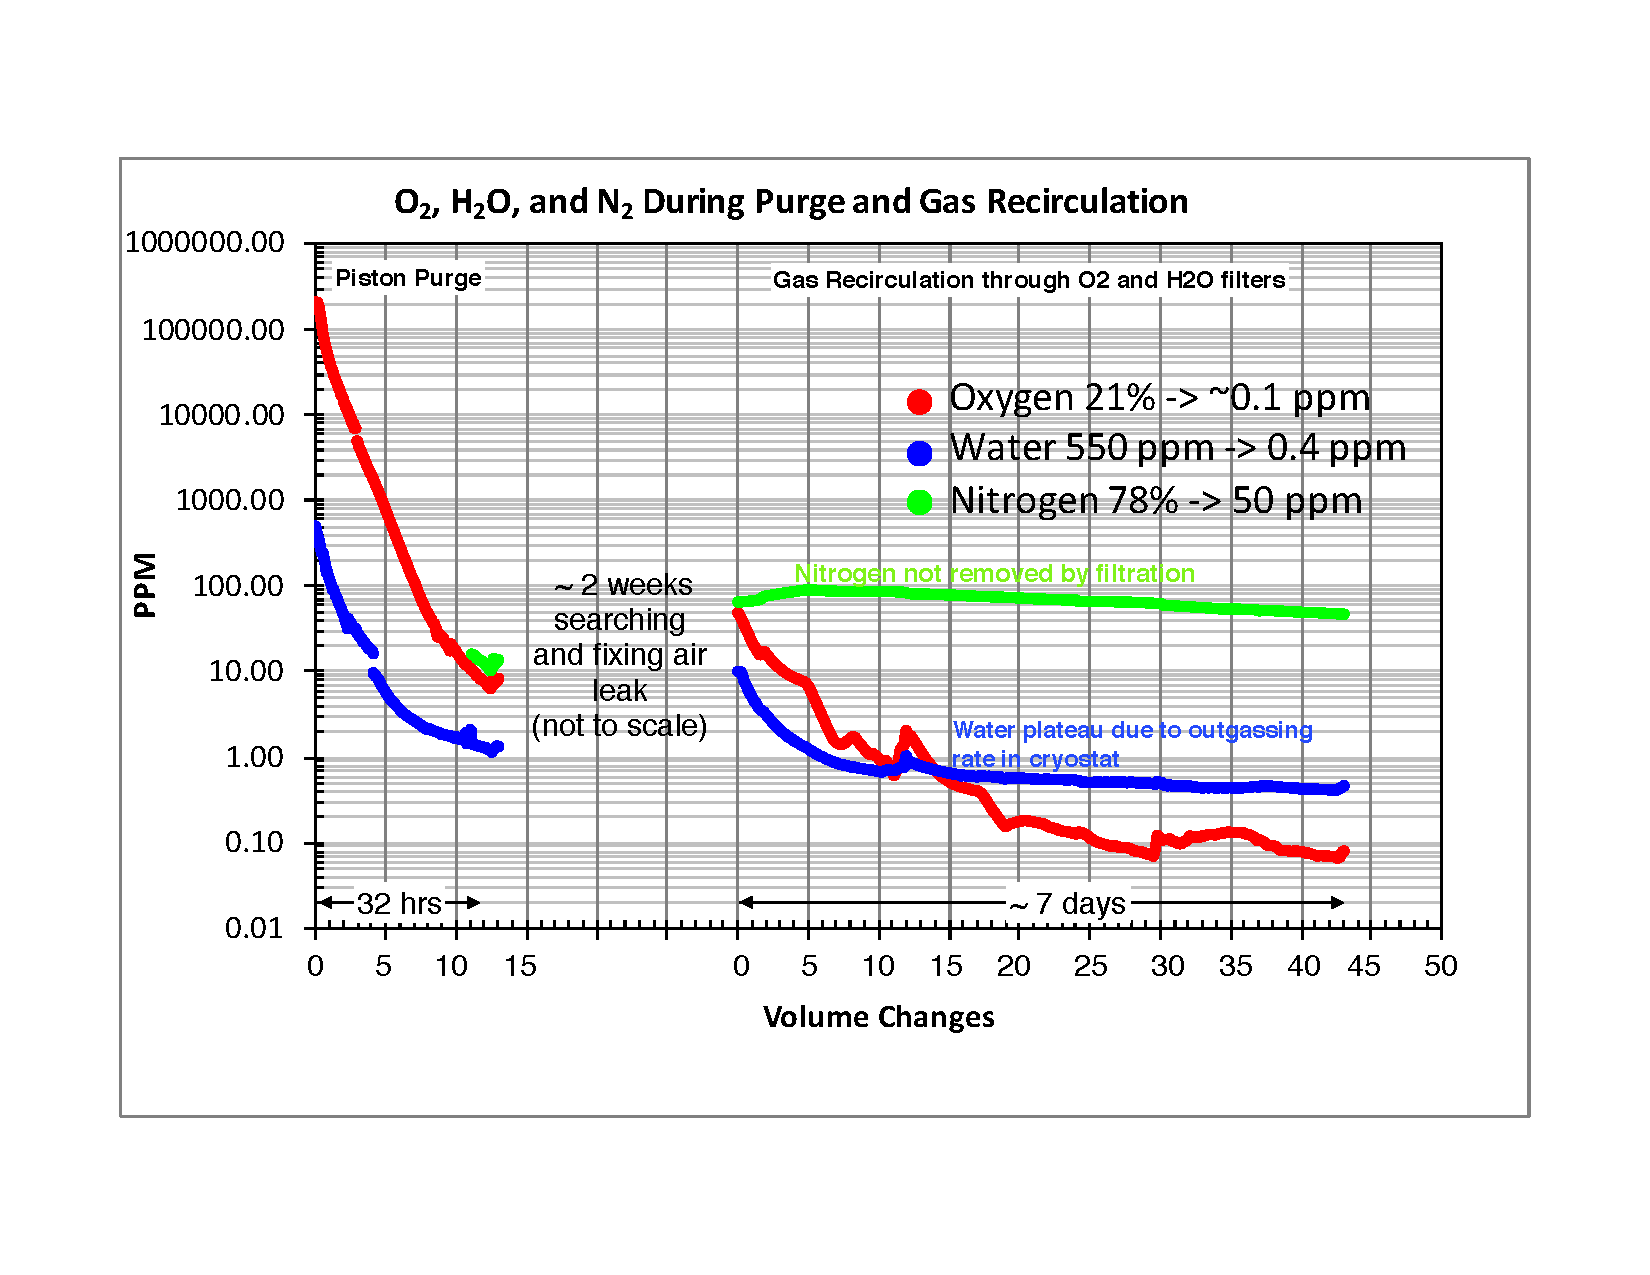
\includegraphics[width=0.7\textwidth]{cisc_Phase1_purge_gas_recirculation}
\end{dunefigure}

\begin{dunefigure}[$\text{O}_2$ just after the \dshort{35t} was filled with \lar]{fig:cisc_O2AnalyzerPrM2_HVRun1}
  {$\text{O}_2$ as measured by a precision $\text{O}_2$ analyzer just after the \dword{35t} cryostat is filled with \lar, continuing with the \lar pump start and beginning of \lar recirculation through the filtration system. As the gas analyzer loses sensitivity, the purity monitor can pick up the impurity measurement. Note that the purity monitor is sensitive to both $\text{O}_2$ and $\text{H}_2\text{O}$ impurities giving rise to its higher levels of impurity.}
  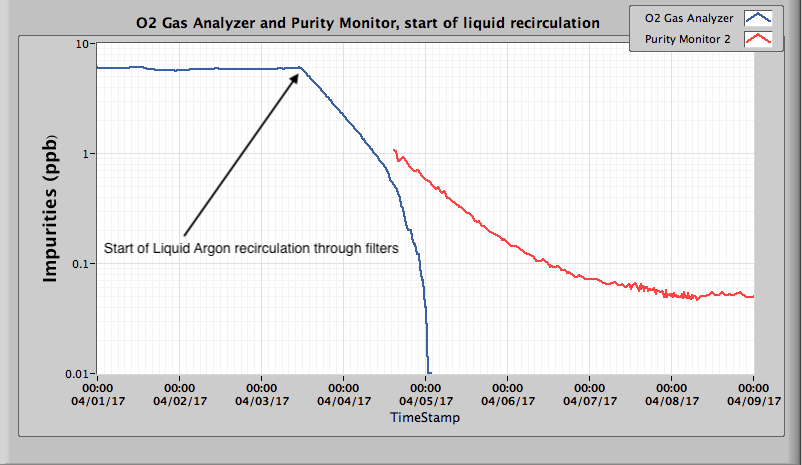
\includegraphics[width=0.7\textwidth]{cisc_O2AnalyzerPrM2_HVRun1.png}
\end{dunefigure}

Because the filling and commissioning of different cryostats will occur at different times, sharing the same gas analyzer installation between them should be possible with minimal effect on the operation on other cryostats. The gas analyzer switchyard can easily switch between cryostat source lines.
%Because 
Since any one gas analyzer covers only one contaminant species and a range of \numrange{3}{4} orders of magnitude, several units are needed both for the three contaminant gases and to cover the ranges seen between cryostat closure and the beginning of \dshort{tpc} operations:
\SI{20}{\percent} to $\lesssim 100$~ppt for $\text{O}_2$,
\SI{80}{\percent} to $\lesssim 1$~ppm for $\text{N}_2$, and
$\sim \SI{1}{\percent}$ to $\lesssim 1$~ppb for $\text{H}_2\text{O}$.
Because the total cost of these analyzers exceeds $\SI{100}[\mathdollar]{k}$, we want to be able to  sample more than a single location or cryostat with the same gas analyzer. At the same time, the tubing run lengths from the sample point should be as short as possible to maintain a timely response for the gas analyzer. This puts some constraints on sharing devices because, for example, argon is delivered at the surface, so a separate gas analyzer may be required there. %at the surface.


%%%%%%%%%%%%%%%%%%%%%55 CAMERAS %%%%%%%%%%%%%%%%%%%%%%%%5
\subsection{Cameras}
% glenn, jim s, chuck
% ALMOST same text in single and dual phase

Cameras provide direct visual information about the state of the
\dword{detmodule} during critical operations and when damage or unusual
conditions are suspected.  Cameras in the \dword{wa105} showed spray from \cooldown
nozzles and the level and state of the \lar as it covered the \dword{crp} \cite{Murphy:20170516}.  A camera was
used in the \dword{lapd} 
cryostat\cite{Adamowski:2014daa} to study \dword{hv} discharges in
\lar and in EXO-100 while a \dword{tpc} was operating
\cite{Delaquis:2013hva}.  Warm cameras viewing \lar from a distance
have been used to observe \dword{hv} discharges in \lar in
fine detail \cite{Auger:2015xlo}.  Cameras are commonly used during
calibration source deployment in many experiments (e.g., the
\kamland ultra-clean system \cite{Banks:2014hra}).

In \dword{dune}, cameras will verify the stability, straightness,
and alignment of the hanging \dword{tpc} structures during \cooldown and
filling; ensure that no bubbling occurs near the \dwords{gp}
(\single) or \dwords{crp} (\dual); inspect the
state of movable parts in the \dword{detmodule} (calibration devices, dynamic
thermometers); and closely inspect parts of the \dword{tpc} after any seismic activity or other unanticipated
event.  For these functions, a set of fixed
cold cameras are used; they are permanently mounted at fixed points in the cryostat
for use during filling and commissioning. A movable, replaceable
warm inspection camera can be deployed through any free
instrumentation flange at any time during the life of the
experiment. 
 
As this is written, the \dword{pddp} installation is nearing completion, and no validation of camera operation in \dword{pddp} is yet available.  \fixme{done now, is validation available?} However,
eleven cameras were deployed in \dword{pdsp}.
They successfully provided views of the detector during filling and throughout
its operation. %The camera designs used in \dword{protodune} will be the basis for the final camera designs used in the \dword{dpmod}.

The following sections describe the design considerations for both cold
and warm cameras and the associated lighting system. \dword{pdsp} camera system designs and performance are also discussed.  
The same basic
designs can be used for both the \dword{spmod} and the \dword{dpmod}. %\single and \dual \dwords{detmodule}.



%%%%%%%%%%%%%%%%%%%%%%%%%%%%%%%%%%%%%%%
\subsubsection{Cryogenic Cameras (Cold)}

The fixed cameras
monitor the following items during filling:
\begin{itemize}
\item positions of corners of \dwords{crp}, cathode, \dwords{fc}, \dwords{gg} (\SI{1}{mm} resolution),
\item relative straightness and alignment of \dwords{crp}, cathode, and \dwords{fc} (\(\lesssim\SI{1}{mm}\)),
\item relative positions of \dword{fc} profiles and resistive sheaths between super-modules (\SI{0.5}{mm} resolution), and 
\item the \lar surface, specifically, the presence of bubbling or debris.
\end{itemize}




One design for the \dword{dune} fixed cameras uses an enclosure similar to
the successful EXO-100 design \cite{Delaquis:2013hva}, which was also
used successfully in the  \dword{lapd} 
and \dword{pdsp} (see Figure~\ref{fig:gen-fdgen-cameras-enclosure}).
A thermocouple in the enclosure allows temperature monitoring and a heating element provides temperature control.  
SUB-D 
connectors are used at the cryostat flanges and the camera enclosure for signal, power, and control connections.


\begin{dunefigure}[A camera enclosure]{fig:gen-fdgen-cameras-enclosure}
  {Top left: a CAD exploded view of a vacuum-tight camera enclosure suitable for cryogenic applications \cite{Delaquis:2013hva}.
    (1) quartz window, (2 and 7) copper gasket, (3 and 6) flanges, (4) indium wires, (5) body piece, (8) signal \fdth.
    Top right: two of the \dword{pdsp} cameras using a stainless steel enclosure. 
    Bottom left: one of the \dword{pdsp} cameras using acrylic enclosure.
    Bottom right: a portion of an image taken with \dword{pdsp} camera 105 showing a purity monitor mounted outside the \dword{apa} on the beam left side. This photo was taken with \dword{pdsp} completely filled.
  }
  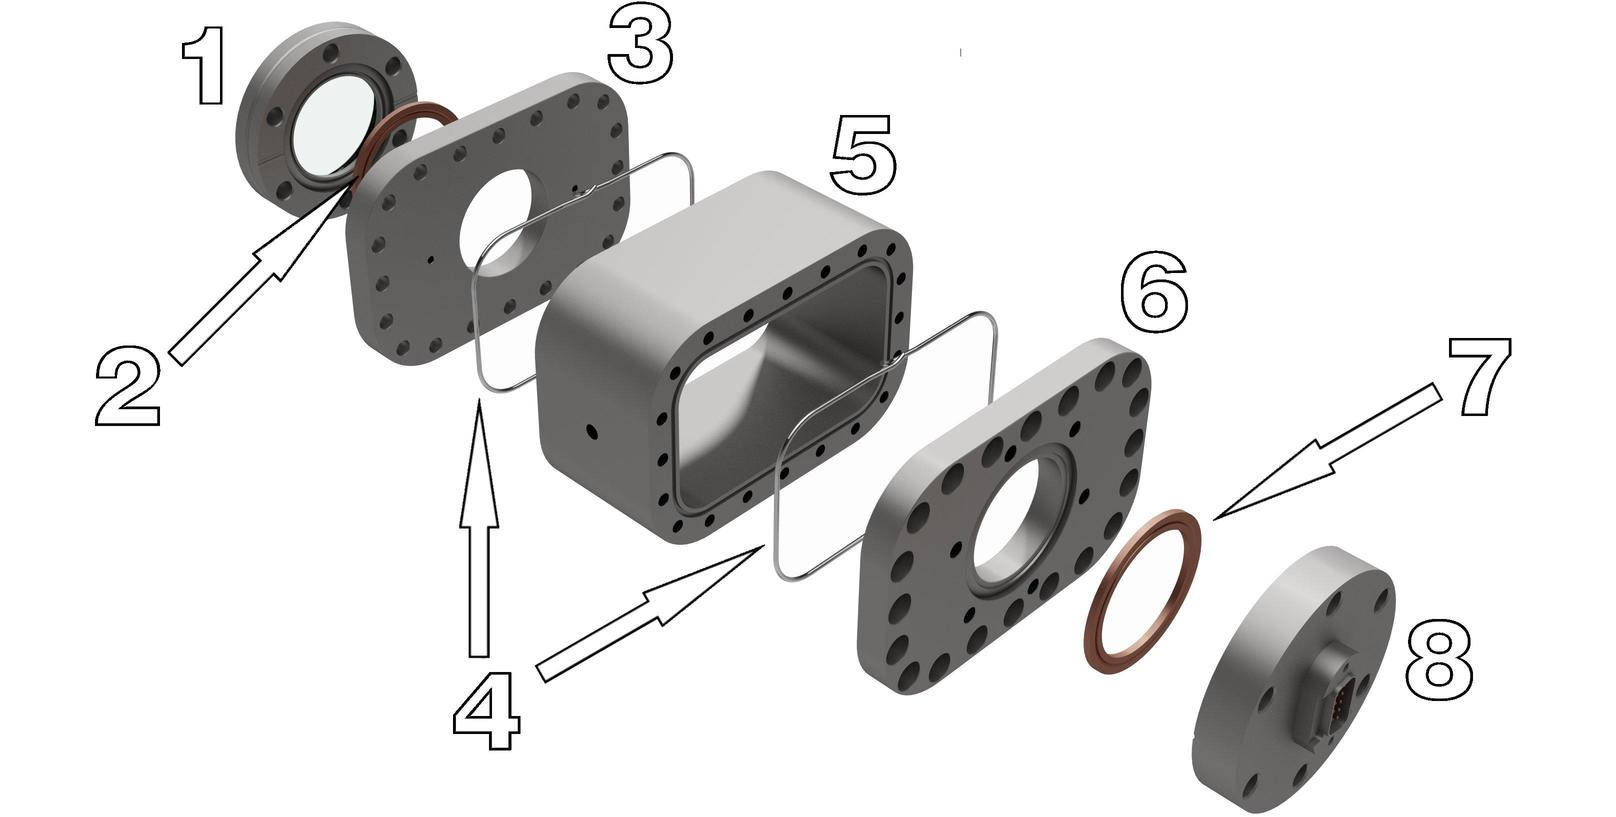
\includegraphics[width=0.4\textwidth]{exo100-camera-case}%
  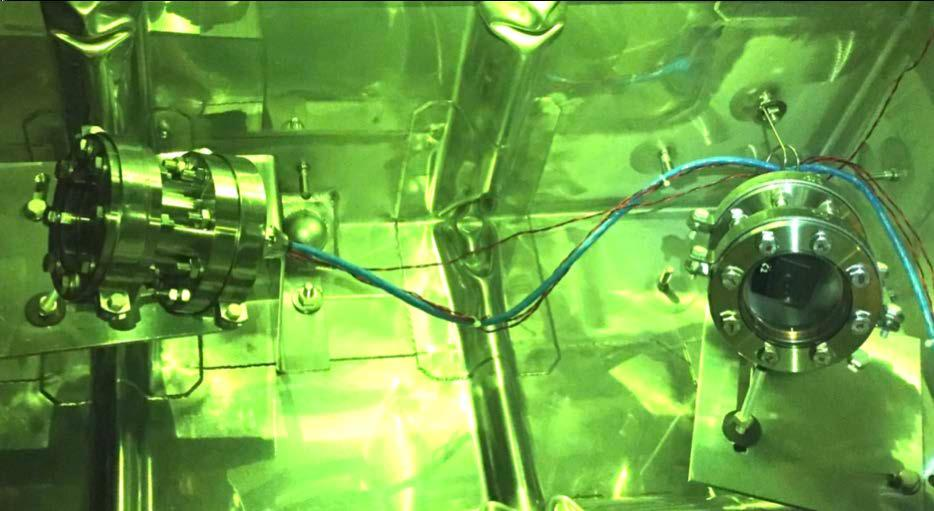
\includegraphics[width=0.4\textwidth]{edgar-cameras}\\
  \hfill 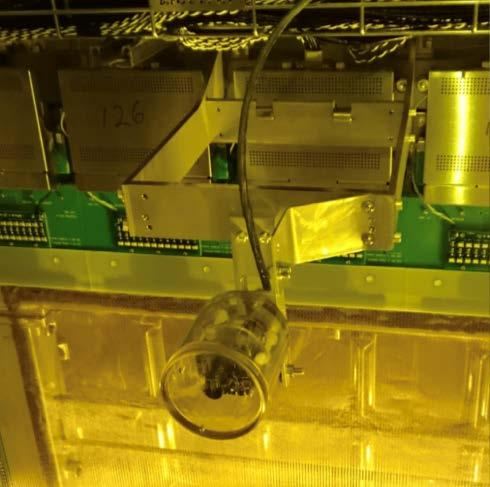
\includegraphics[width=0.22\textwidth]{bo-camera}%
  \hfill 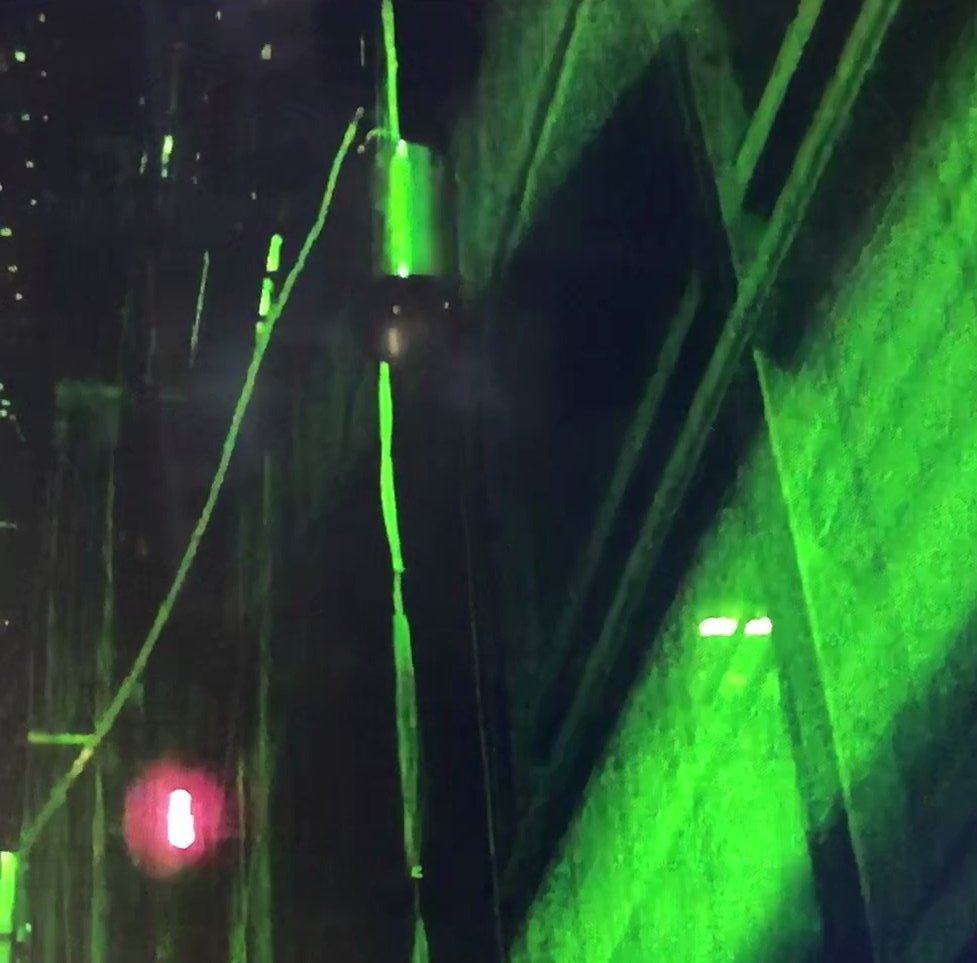
\includegraphics[width=0.22\textwidth]{camera-105-purmon-orig-rot-crop}%
  \hfill
\end{dunefigure}

An alternative design uses an acrylic enclosure.
This design was used successfully in \dword{pdsp} (see Figure~\ref{fig:gen-fdgen-cameras-enclosure}, bottom left).

All operate successfully, including those at the bottom of the cryostat.  %Please note that the \dword{dune} \dword{fd} 
The \dword{fd} modules will be twice as deep as \dword{protodune}, and therefore cameras observing the lowest surfaces of the \dword{fc} must withstand twice the pressure.

Improved designs for the cold cameras will be tested in \dword{pddp} and \dword{citf} for improved imaging including focus adjustment, and in \dword{citf} for pressure resistance, during 2020. 

%%%%%%%%%%%%%%%%%%%%%%%%%%%%%%%%%%%%%%%%%%%%%%%5
\subsubsection{Inspection Cameras (Warm)}

The inspection cameras are intended to be as versatile as possible.
The following %locations 
inspections have been identified as likely uses:
%to be of interest:
\begin{itemize}
\item status of \dword{hv} \fdth and cup,
\item status and relative position of \dword{fc} profiles, resistive sheaths between \dword{fc} super-modules (\SI{0.5}{mm} resolution),
\item vertical deployment of calibration sources,
\item status of thermometers, especially dynamic thermometers,
\item \dword{hv} discharge, corona, or streamers on \dword{hv} \fdth, cup, or \dword{fc},
\item relative straightness and alignment of \dwords{crp}, cathode, and \dword{fc} (\SI{1}{mm} resolution), and
\item gaps between \dword{crp} frames (\SI{1}{mm} resolution).
\end{itemize}

Unlike the fixed cameras, the inspection cameras operate only as
long as any inspection; the cameras can be replaced in case of failure.  It
is also more practical to keep the cameras continuously warmer than
 \SI{-150}{\celsius} during deployment; this allows use of  %and therefore we willhave 
commercial cameras, %more easily, e.g., %.  For example, we could deploy 
e.g., cameras of the same model were used successfully to observe discharges
in \dword{lar} from \SI{120}{cm} away \cite{Auger:2015xlo}.


The inspection cameras use the same basic
enclosure design as cold cameras, but the cameras are mounted on a movable
fork, so each camera can be inserted and removed from the cryostat
using a design similar to the dynamic temperature probes (see
 Figures~\ref{fig:gen-fdgen-cameras-movable} (left) and
 ~\ref{fig:fd-slow-cryo-sensor-mount}).  To avoid contaminating the
\lar with air, the entire system is sealed, and the
camera can only be deployed through a \fdth equipped with a gate
valve and a purging system, similar to the one used in the vertical axis
calibration system at \kamland~\cite{Banks:2014hra}. The entire system
is  purged with pure argon gas before the gate valve is opened.

\begin{dunefigure}[Inspection camera design]{fig:gen-fdgen-cameras-movable}
  {Left: An overview of the inspection camera design using a sealed deployment system opening directly into the cryostat. Right: A photograph of the \dword{pdsp} warm inspection camera acrylic tube immediately before installation; the acrylic tube is sealed with an acrylic dome at the bottom and can be opened at the top.}
  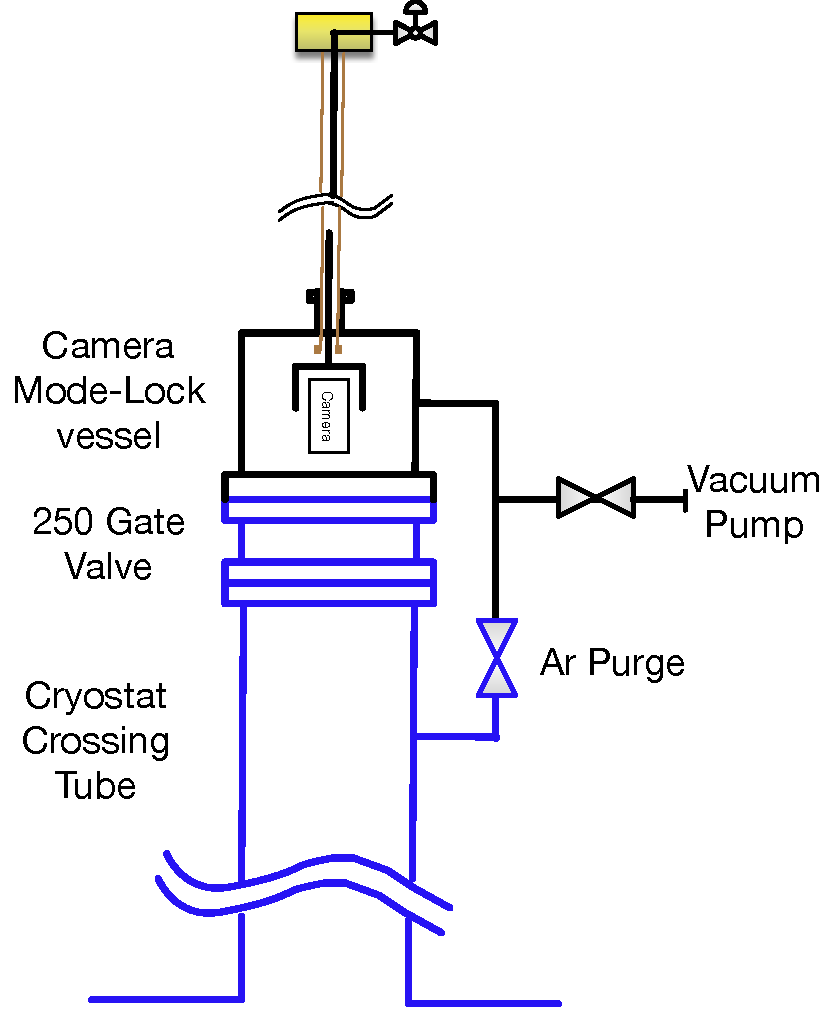
\includegraphics[height=0.3\textheight]{Camera-Sketch}%
  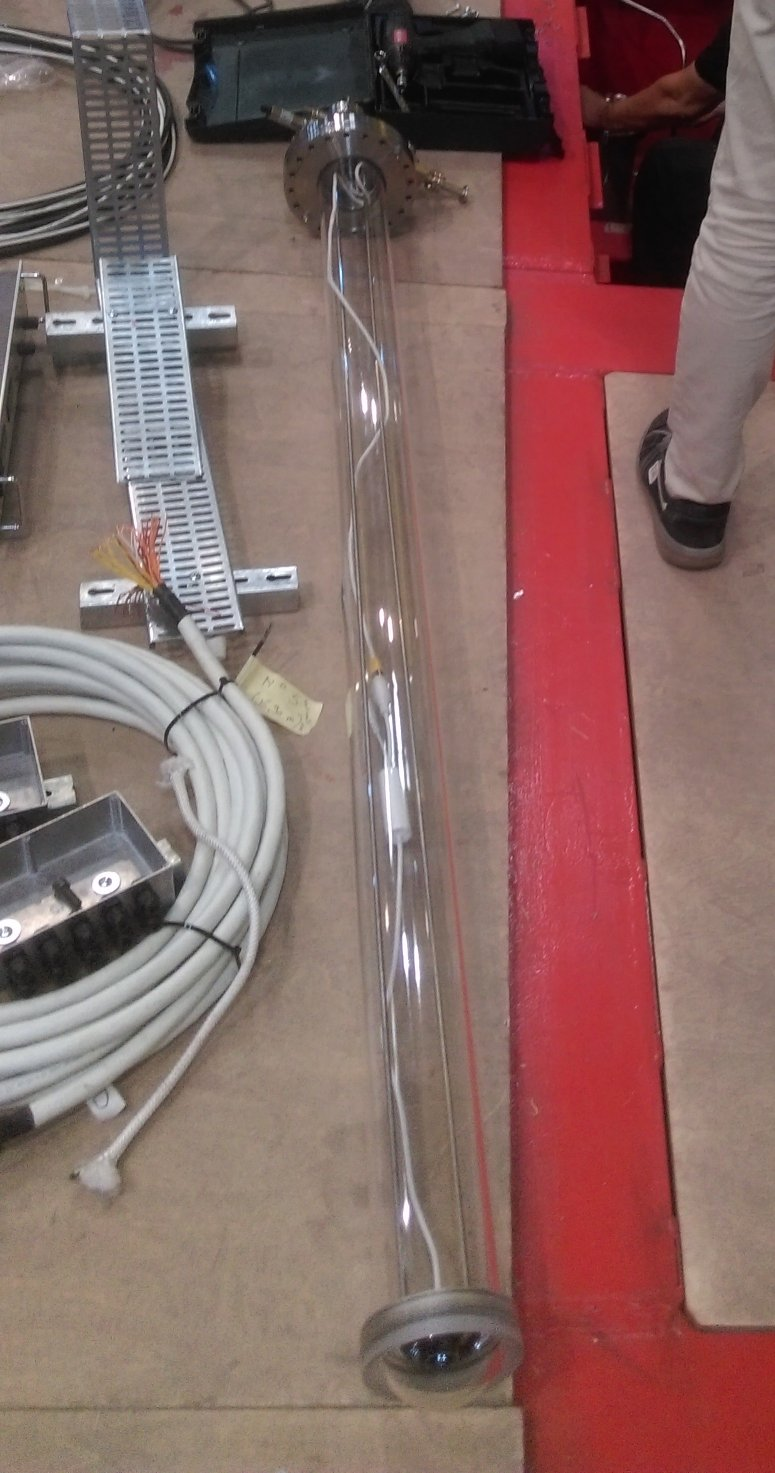
\includegraphics[height=0.3\textheight]{cisc-pdsp-camera-tube}%
\end{dunefigure}

Motors above the flange allow the fork to be rotated and moved vertically to position the camera. 
 A chain drive system with a motor
mounted on the end of the fork allows the camera assembly to tilt, 
creating a point-tilt mount that can be moved vertically.
With the space above the cryostat flanges and the
thickness of the cryostat insulation, cameras can be moved vertically up to
\SI{1}{m} inside the cryostat.
The motors for rotation and vertical motion are outside the sealed
volume, coupled mechanically using ferrofluidic seals, thus reducing any risk of
contamination and allowing manual rotation of the vertical
drive if the motor fails.  

An alternative design was demonstrated in \dword{pdsp}. In this design, the warm camera is contained inside a gas-tight acrylic tube inserted into the feedthrough, so a gate valve or a gas-tight rotatable stage is not needed; the warm cameras can thus be removed for servicing or upgrade at any time. Figure~\ref{fig:gen-fdgen-cameras-movable} (right) shows an acrylic tube enclosure and camera immediately before deployment.
Three such tubes were installed in \dword{pdsp}, and cameras with fisheye lenses were operated successfully.  One camera was removed without any evidence of contamination of the \dword{lar}.


Improved designs for the inspection cameras will be tested in the \dword{citf} and \dword{pdsp} during 2020 and 2021, focusing particularly on longevity, camera replaceability, and protection of the \dword{lar}.

%%%%%%%%%%%%%%%%%%%%%%%%%%%%%%%%%%%%%%%
\subsubsection{Light-emitting system}
%%% same text as dual-phase
The light-emitting system uses \dwords{led} to illuminate
the parts of the %\dword{fd} 
\dword{detmodule} in the camera's field of view with selected
wavelengths (IR and visible) that cameras can detect.  Performance criteria for the light-emission system include the efficiency with which the cameras can detect the light and the need to avoid
adding heat to the cryostat. Very high-efficiency
\dwords{led}   
help reduce heat generation; one \SI{750}{nm} \dword{led} \cite{lumileds-DS144-pdf}
has a specification equivalent to
\SI{33}{\%} conversion of electrical input power to light.
% CEL: 1W electrical gives 425mW blue flux, power limit from SMD package thermal resistance of 8C/W to have max 1C increase at LED. CREE Xlamp XP-E model

While data on how well \dwords{led} perform at cryogenic temperatures
is sparse, some studies of NASA projects~\cite{Carron:2017zzz}
indicate that \dwords{led} are more efficient at low temperatures and
that emitted wavelengths may change, particularly for blue
\dwords{led}.  In \dword{pdsp}, amber \dwords{led} were observed  to
emit green light at \dword{lar} temperature (see bottom right photo
in \ref{fig:gen-fdgen-cameras-enclosure}).  To avoid degradation of
wavelength-shifting materials in the \dword{pds}, short wavelength
\dwords{led} are not used in the \dword{fd}; \dwords{led} will be tested
in \dword{ln} to ensure their wavelength is long enough.


\dwords{led} are placed in a ring around the outside of each
camera, pointing in the same direction as the lens, to 
illuminate nearby parts of the \dword{detmodule} within the camera's field of
view. Commercially available \dwords{led} exist with
a range of angular spreads that can match the needs of the
cameras without additional optics.

Additionally, chains of \dwords{led} connected in series and driven with a
constant-current circuit are used for broad illumination, with each
\dword{led} paired in parallel with an opposite polarity \dword{led} and a resistor
(see Figure~\ref{fig:cisc-LED}).
This gives two different wavelengths of illumination using a single chain simply by changing the direction of the drive current and allows continued use of an \dword{led} chain even if individual \dwords{led} fail.

\begin{dunefigure}[Example schematic for LED chain]{fig:cisc-LED}
  {Example schematic for LED chain, allowing failure tolerance and two LED illumination spectra.}
  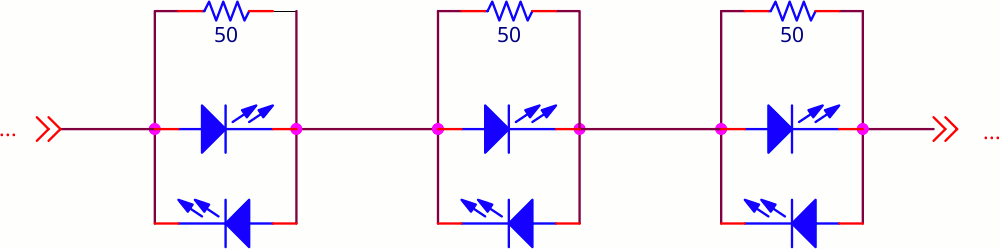
\includegraphics[width=0.6\textwidth]{cisc_led.png}
\end{dunefigure}


%%%%%%%%%%%%%%%%%% CRYOGENIC Instrumentation TEST FACILITY %%%%%%%%%%%%%%%%%%%
\subsection{Cryogenic Instrumentation Test Facility}
% same for SP and DP
% alan h
The \dword{cisc} consortium plans to build a \dfirst{citf} at \dword{fnal} to facilitate testing of various cryogenic instrumentation devices and small-scale assemblies of \dword{cisc} systems. 
%The \dfirst{citf} at 
In the past and recent times, various test facilities at \dword{fnal} have provided access to small ($<\,\SI{1}{ton}$) to intermediate ($\sim\,\SI{1}{ton}$) volumes of purified \dword{tpc}-grade \dword{lar}, required for %. Hardware that requires this high-purity liquid includes 
any device intended for drifting electrons for millisecond periods. 

The \dword{pab} facility at \dword{fnal} houses the \dword{iceberg} \SI {3000} {liter} cryostat that allows fast turnaround for testing of the \dword{dune} \dword{ce}. 

The \dword{pab} facility also includes \dword{tallbo} (\SI {450} {liter}), Blanche (\SI {500} {liter}), and Luke (\SI {250} {liter}) cryostats. %All these cryostats are available for outside use.
In the recent past, Blanche has been used for \dword{hv} studies,  \dword{tallbo} for \dword{pd} studies, and Luke for the material test stand work. These studies have contributed to the design and testing of  \dword{pdsp} components.
%\fixme{CP: DP facility for CRP testing could be added; SG: that would fall under CRP scope}

\subsection{Validation in ProtoDUNE}
\label{sec:pddp-cryo-valid}

%\fixme{SG/ACV:DONE; New section added for DP}

Design validation and testing of many planned \dword{cisc} systems for the \dword{dune} \dword{dp} \dword{fd} will be done using data from both \dword{pdsp} and \dword{pddp} detectors as discussed below.

\begin{itemize}
    \item  Level Meters: The same differential pressure level meters that are already validated in \dword{pdsp} will be used in the \dword{dpmod}. The same capacitive level meters currently used in \dword{pddp} will be used in the \dword{dpmod}. These will be validated in the upcoming \dword{pddp} run. 
    
    \item Pressure Meters (GAr): The same high-precision pressure sensors which are already validated in \dword{pdsp} will be used in the \dword{dpmod}.
    
    \item Gas Analyzers:  The same gas analyzers currently used in \dword{pdsp} will be used in the \dword{dpmod}. They have already been validated.
    
    \item Vertical array of thermometers in GAr: The same design of vertical array of thermometers currently used in \dword{pddp} will be used in the \dword{dpmod} but with different distribution density. This design will be validated with \dword{pddp} data.
    
    \item High-precision thermometer arrays in \lar: The static and dynamic T-gradient thermometers discussed in previous sections are not yet installed in \dword{pddp}, but the plan is to deploy them in the \dword{dpmod}. Therefore, the validation of these devices will be performed using \dword{pdsp} data and can also be tested in future running of \dword{pddp}.
    
    \item Purity monitors: The purity monitors are being validated at both \dword{pdsp} and \dword{pddp}. Currently, \dword{pdsp} and \dword{pddp} are using slightly different designs. For the \dword{dpmod}, the plan is to use the same design as \dword{pdsp} along with some improvements such as longer drift purity monitors to increase the range of measured lifetime values.  \dword{protodune2} at \dword{cern} provides opportunities to
	      test any improvements to the design. 
    %\todo{CP:ProtoDUNE-DP is already testing possible improvements, as different silver cathodes}
  \item Cameras: various types of cameras are being actively developed in both \dword{pdsp} and \dword{pddp} so these detectors will perform validation of the   designs. Future improvements can be tested in \dword{protodune2} at \dword{cern}. % \dword{pdsp} and \dword{pddp} run 2 phaseat CERN.
\end{itemize}

%%%%%%%%
\section{Slow Controls}
% same for SP and DP

The slow controls system collects, archives, and displays data from
a broad variety of sources and provides real-time status, alarms, and warnings for detector operators. The slow control system also provides control for %some detector components of the detector systems 
items such as \dword{hv} systems, \dword{tpc} electronics, and \dword{pd} systems. Data are acquired via network interfaces.  Figure~\ref{fig:gen-slow-controls-diagram} shows connections between major parts of the slow controls system and other systems. Hardware, infrastructure, and software are the three main components of the slow controls system. %, each of which are described in this section.

\begin{dunefigure}[Slow controls connections and data]{fig:gen-slow-controls-diagram}
{Typical slow controls system connections and data flow.}
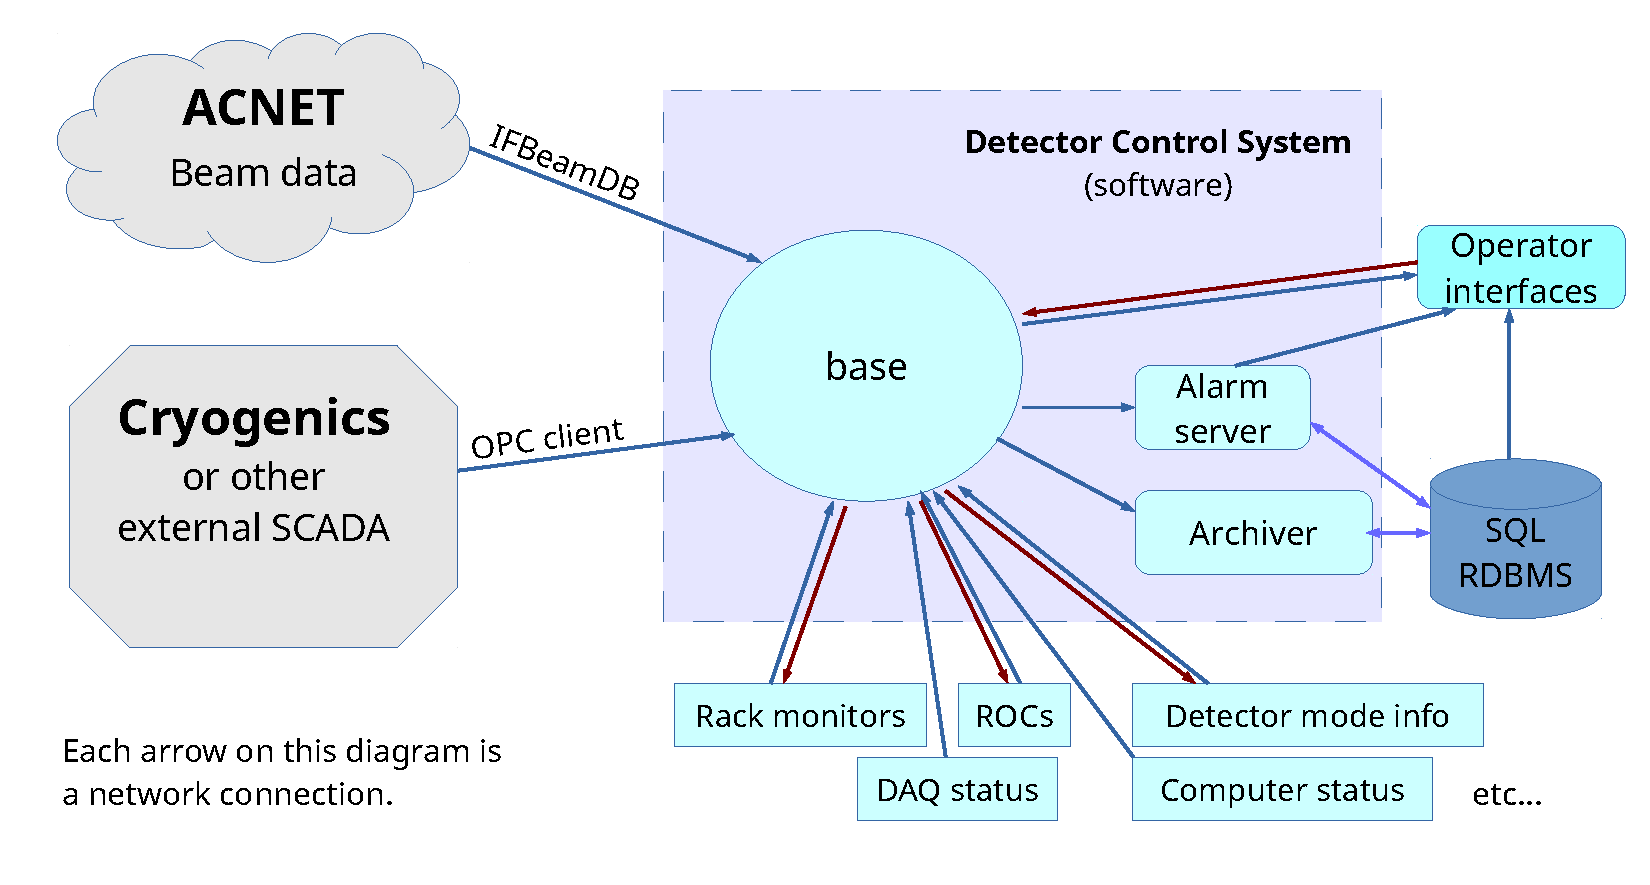
\includegraphics[width=0.7\textwidth]{cisc_slow-controls-diagram}
\end{dunefigure}

The \dword{pdsp} detector control system\cite{pdspdcs_proc}  met its operational requirements fully. %the requirements for operating \dword{pdsp}. 
Section~\ref{sec:cisc-slow-control-pdsp} provides a short description of the \dword{pdsp} slow controls and its performance.

%%%%%%%%%%%%%%%%%%%%%%%%%%%%%%%%%%%
 \subsection{Slow Controls Hardware}
\label{sec:fdgen-slow-cryo-hdwr}

%A modest amount of dedicated hardware is envisioned for 
Slow controls requires a modest amount of dedicated hardware, mostly for rack monitoring,  %Additionally, slow controls will always 
and a small amount of dedicated network and
computing hardware. % as described below. 
Slow controls also relies on common
infrastructure as described in
Section~\ref{sec:fdgen-slow-cryo-slow-infra}.

%%%%%%%%%%%%%%%%%
\subsubsection{Dedicated Monitoring Hardware}

Every rack (including those in the \dword{cuc}) should have dedicated hardware to monitor rack parameters like rack protection system, rack fans, rack air temperatures, thermal interlocks with power supplies, and any interlock bit status monitoring needed for the racks. For the racks in the \dword{cuc} server room, this functionality is built into the proposed water cooled racks, much like what is already in place at \dword{protodune}.  For the racks on the detector itself, the current plan is to design and install a custom-built 1U rack-mount enclosure containing a single-board computer to control and monitor various rack parameters. Such a system has been successfully used in \dword{microboone}. The design is being improved for the \dword{sbnd} experiment (see Figure~\ref{fig:slow-controls-rack-box}). Other slow controls hardware includes interfacing cables like adapters for communication and debugging and other specialized cables like \dword{gpib} 
or National Instruments cables. The cable requirements must be determined in consultation with other groups once hardware choices for various systems are finalized.

\begin{dunefigure}[Rack monitoring box prototype for the SBND; based on MicroBooNE design]{fig:slow-controls-rack-box}
{Rack monitoring box prototype in development for the \dshort{sbnd} experiment based on the original design from \dshort{microboone}.}
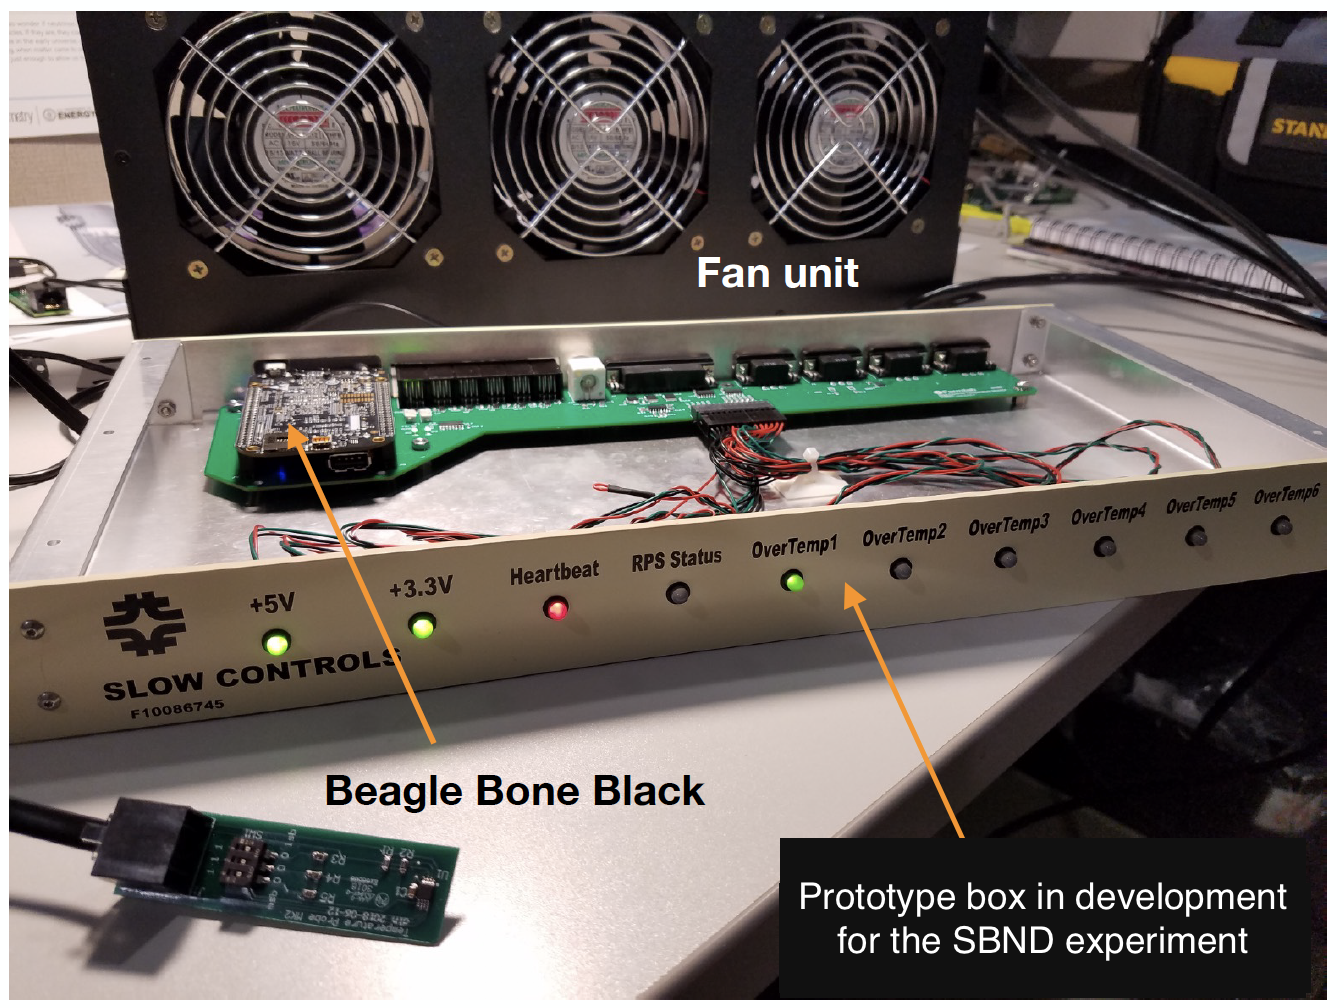
\includegraphics[width=0.6\textwidth]{cisc-slow-controls-rackbox}
\end{dunefigure}


% % % % Alec
\subsubsection{Slow Controls Network Hardware}
\label{sec:fdgen-slow-cryo-slow-network}
The slow controls data originates from the cryogenic instrumentation and from other systems as listed in Table~\ref{tab:gen-slow-quant}. This data is collected by software running on servers
(see Section~\ref{sec:fdgen-slow-cryo-slow-compute})
housed in the underground data room in the \dword{cuc},
where data is archived in a central \dword{cisc} database.
The instrumentation data is transported over
conventional network hardware from any sensors located in the cryogenics
plant.  However, we must remain aware of grounding and noise in readouts in the racks on top of the
cryostats.  Therefore, each
rack on the cryostat has a small network switch that sends
any network traffic from that rack to the \dword{cuc} via a fiber transponder.
This is the only network hardware specific to slow controls and will be provided by %the laboratory's
\dword{surf}'s   
general computing infrastructure. % managed by project \dword{tc}. 
The network infrastructure requirements are described in
Section~\ref{sec:fdgen-slow-cryo-slow-infra}.

% % % % Alec
\subsubsection{Slow Controls Computing Hardware}
\label{sec:fdgen-slow-cryo-slow-compute}
Two servers (a primary server and a replicated backup) suitable for the relational database discussed
in Section~\ref{sec:fdgen-slow-cryo-sw} are located in the \dword{cuc} data
room along with an additional
two servers for the \dword{fe} monitoring interface. These additional servers would cover assembling dynamic \dword{cisc} monitoring web pages from adjacent
databases.  Yet another server will be needed to run back-end I/O.  Any special purpose software, such as iFix used by the cryogenics experts, would
also run here. One or two additional servers should accommodate these programs.
% (The exact number of iFix machines will be determined based
% on input from the LBNF cryogenics experts.)
Replicating this setup for each module would make commissioning and independent operation easier, accommodate different module
designs (with resulting differences in database tables), and ensure
sufficient capacity.  These four sets of networking hardware would fit tightly into one rack or very comfortably into two.  \fixme{No cost info in TDR: Using the requirements from \dword{cisc}, the \dword{daq} consortium will provide the needed cost estimates for servers and racks. }



%%%%%%%%%%%%%%%%%%%%%%%%%%%%%%%%%%%
% Alec
\subsection{Slow Controls Infrastructure}
\label{sec:fdgen-slow-cryo-slow-infra}

The data rate will be in the range of tens of kilobytes per second, given the total number of slow controls quantities and the update rate  
(see Section~\ref{sec:fdgen-slow-cryo-quant}), placing minimal demands
on local network infrastructure.
Network traffic out of  \dword{surf} to \dword{fnal} will primarily be database calls
to the central \dword{cisc} database, either from monitoring applications or from
database replication to the offline version of the \dword{cisc} database.  This
traffic requires little bandwidth, so the proposed general purpose
links both out of the %mine 
underground area at  \dword{surf} and back to \dword{fnal}  can accommodate the traffic.

Up to two racks of space and appropriate power and cooling are
available in the \dword{cuc}'s \dword{daq} server room for \dword{cisc} use. This is ample space (see Section~\ref{sec:fdgen-slow-cryo-slow-compute}).


%%%%%%%%%%%%%%%%%%%%%%%%%%%%%%%%%%
% Sowjanya
\subsection{Slow Controls Software}
\label{sec:fdgen-slow-cryo-sw}


To provide complete monitoring and control of detector subsystems, the slow controls software includes
%
\begin{itemize}
 \item the control systems base for input and output operations
  and defining processing logic, scan conditions, and alarm conditions;
 \item an alarm server to monitor all channels and send alarm
  messages to operators;
 \item a data archiver for automatic sampling and storing values for history tracking; and 
 \item an integrated operator interface providing display panels for
  controls and monitoring.
\end{itemize}

In addition, the software must be able to 
interface indirectly with external systems (e.g., cryogenics control
system) and databases (e.g., beam database) to export data into
slow controls process variables (or channels) for archiving and status
displays. This allows us to integrate displays and warnings into one
system for the experiment operators and %to provide 
provides integrated
archiving for sampled data in the archived database. As one possibility, an input output controller running on a central \dword{daq}
server could provide soft channels for these data.
Figure~\ref{fig:gen-slow-controls-diagram} shows a typical workflow of a
slow controls system.

The key features of the software require highly evolved software designed to manage real-time data exchange, scalable
to hundreds of thousands of channels sampled at intervals of hours to seconds as needed. The software
must be well documented, supported, and reliable. The base
software must also allow easy access to any channel by name. The
archiver software must allow data storage in a database with
adjustable rates and thresholds so data
for any channel can be easily retrieved using channel name and time range. Among other key
features, the alarm server software must remember the state, support an
arbitrary number of clients, and provide logic for delayed alarms and
acknowledging alarms. A standard naming
convention for channels will be part of the software to help handle large
numbers of channels and subsystems.



The \dword{protodune} detector control system software \cite{pdspdcs_proc}
provides a prototype for %this required
the \dword{fd} slow controls software.
In \dword{protodune}, the unified control system base is WinCC OA \cite{winccoa}, a
commercial toolkit used extensively at \dword{cern}, with device interfaces
supported using several standardized interface protocols. A more detailed description is in Section~\ref{sec:cisc-slow-control-pdsp} below.
WinCC OA is our baseline for the \dword{fd} slow control software.
EPICS \cite{epics7} is an alternative controls system which also meets the specifications; it is used in other neutrino experiments including \dword{microboone}\cite{microboone} and \dword{nova}\cite{Lukhanin:2012fp}. 

%%%%%%%%%%%%%%%%%%%%%%%%%%%%%%%%%%
% Ed T
\subsection{Slow Controls Quantities}
\label{sec:fdgen-slow-cryo-quant}

% starter text from Glenn

%\fixme{"3rd draft" or supplement : update total no. of variables once you here from Giovanna/Xavier}

The final set of quantities to monitor will ultimately be determined
by the subsystems being monitored, documented in appropriate  interface control documents (ICDs), and continually revised based on operational experience.  The total number of quantities to monitor has been roughly estimated by taking the total number monitored in \dword{pdsp}~\cite{pdspdcs_proc}, 7595 as of Nov. 19, 2018, and scaling by the detector length and the number of planes, giving approximately 150,000 per \dword{detmodule}. In the case of \dword{pddp}, we do not have the exact total number monitored yet, but the expectation is that the \dword{dp} numbers should not deviate substantially from \dword{sp} and in fact maybe lower since the total number of channels is lower. We think the \dword{pdsp}-based estimate can be considered as an upper limit for the \dword{dp}.
Quantities should update on average no more than once per minute.
Transmitting a single update for each channel at that rate translates to a few thousand updates per second, or a few tens of thousands of bytes per second. While this is not a significant load on a network with an efficient slow controls protocol, it would correspond to approximately \SI{1}{TB} per year per \dword{detmodule} if every timestamp and value were stored.
The actual data volume will be lower because values are stored only if they vary from previous values by more than an amount that is adjustable channel-by-channel.
Database storage also allows data to be sparsified later.
No slow controls data is planned to be written to the \dword{daq} stream.
With careful management of archiving thresholds for each quantity monitored and yearly reduction of stored sample time density, the retained data volume can be reduced to a few TB over the life of the experiment.

The subsystems
to be monitored include the 
cryogenic instrumentation
described in this chapter, the other detector systems, and relevant
infrastructure and external devices. Table~\ref{tab:gen-slow-quant}
lists the quantities expected from each system.

\begin{dunetable}
[Slow controls quantities]
{p{0.3\textwidth}p{0.6\textwidth}}
{tab:gen-slow-quant}
{Slow controls quantities.}
System & Quantities \\ \toprowrule
\multicolumn{2}{l}{\bf Detector cryogenic instrumentation } \\ \specialrule{1.5pt}{1pt}{1pt}
Purity monitors & anode and cathode charge, bias voltage and current, flash lamp status, calculated electron lifetime \\ \colhline
Thermometers & temperature, position of dynamic thermometers \\ \colhline
Liquid level & liquid level \\ \colhline
Pressure meters & pressure readings \\ \colhline
Gas analyzers & purity level readings \\ \colhline
Cameras & camera voltage and current draw, temperature, heater current and voltage, lighting current and voltage \\ \toprowrule
\multicolumn{2}{l}{\bf Other detector systems } \\ \specialrule{1.5pt}{1pt}{1pt}
Cryogenic internal piping & \fdth gas purge flow and temperature \\ \colhline
\dword{hv} systems & drift \dword{hv} voltage and current, end-of-field cage current and bias voltage, electron diverter bias, ground plane currents \\ \colhline
\dword{tpc} electronics & voltage and current to electronics \\ \colhline
\dword{pd} & voltage and current for photodetectors and electronics \\ \colhline
\dword{daq} & warm electronics currents and voltages, run status, \dword{daq} buffer sizes, trigger rates, data rates, GPS status, computer and disk health status, other health metrics as defined by \dword{daq} group \\ \colhline
\dword{crp} / \dword{apa} & bias voltages and currents \\ \toprowrule
\multicolumn{2}{l}{\bf Infrastructure and external systems } \\ \specialrule{1.5pt}{1pt}{1pt}
Cryogenics (external) & status of pumps, flow rates, inlet and return temperature and pressure (via \dword{opc-ua} or similar \dword{scada} interface) \\ \colhline
Beam status & protons on target, rate, target steering, beam pulse timing (via \dword{ifbeam}) \\ \colhline
Near detector & near detector run status (through common slow controls database) \\ \colhline
Rack power and status & power distribution unit current and voltage, air temperature, fan status if applicable, interlock status \\ \colhline
\multicolumn{2}{l}{\bf Detector calibration systems } \\ \specialrule{1.5pt}{1pt}{1pt}
Laser & laser power, temperature, operation modes, other system status as defined by calibration group\\ \colhline
External neutron source  & safety interlock status, power supply monitoring, other system status as defined by calibration group \\ \colhline
External radioactive source & system status as defined by calibration group\\
\end{dunetable}

%%%%%%%%%%%%%%%%%%%%%%%%%%%%%%%%%%
% Sowjanya and Anselmo
\subsection{Local Integration}
\label{sec:fdgen-slow-cryo-slow-loc-integ}



The local integration of slow controls consists entirely of software
and network interfaces with systems that are outside the scope of the \dword{detmodule}.
This includes the following:
\begin{itemize}
\item readings from the \dword{lbnf}-managed external cryogenics systems, for status of pumps, flow rates, inlet, and return temperature and pressure, which are implemented via \dword{opc-ua} or a similar \dword{scada} interface; 
\item beam status, such as protons-on-target, rate, target steering, and beam pulse timing, which are retrieved via \dword{ifbeam}; 
and \item near detector status, which can be retrieved from a common slow controls database.
\end{itemize}
%
Integration occurs after both the slow controls and non-detector
systems are in place.  The \dword{lbnf}-\dword{cisc} interface is managed by the
cryogenics systems working group in \dword{cisc} (see Section~\ref{sec:cisc-slow-controls-org}), which includes members from both \dword{cisc} and \dword{lbnf}. 
The \dword{ifbeam} DB interface for slow controls is an already well established method used in \dword{microboone}, \dword{nova}, and other \dword{fnal} experiments. An internal \dword{nd}/\dword{fd} working group can be established 
to coordinate detector status exchange between the near and far sites.

%%%%%%%%%%%%%
\subsection{Validation in ProtoDUNE}
\label{sec:cisc-slow-control-pdsp}

The \dword{protodune} slow control system has met
all requirements for operation of \dword{pdsp}\cite{pdspdcs_proc} and will be used for \dword{pddp}.  The requirements for \dword{protodune} are
nearly identical to those for the \dword{dpmod} other than
total channel count. Of particular note, the \dword{protodune} slow control system unified a heterogenous set of devices and data sources
through several protocols into a
single control system, as illustrated in
Figure~\ref{fig:cisc-NP04-DCS-topology}. In addition to what
the figure shows, data were also acquired from external cryogenics and beam
systems.  The topology and data flow of the system matches the general
shape shown in Figure~\ref{fig:gen-slow-controls-diagram}.

\begin{dunefigure}[Diagram of the ProtoDUNE-SP control system topology]{fig:cisc-NP04-DCS-topology}
{Diagram of the \dword{pdsp} control system topology, from \cite{pdspdcs_proc}.}
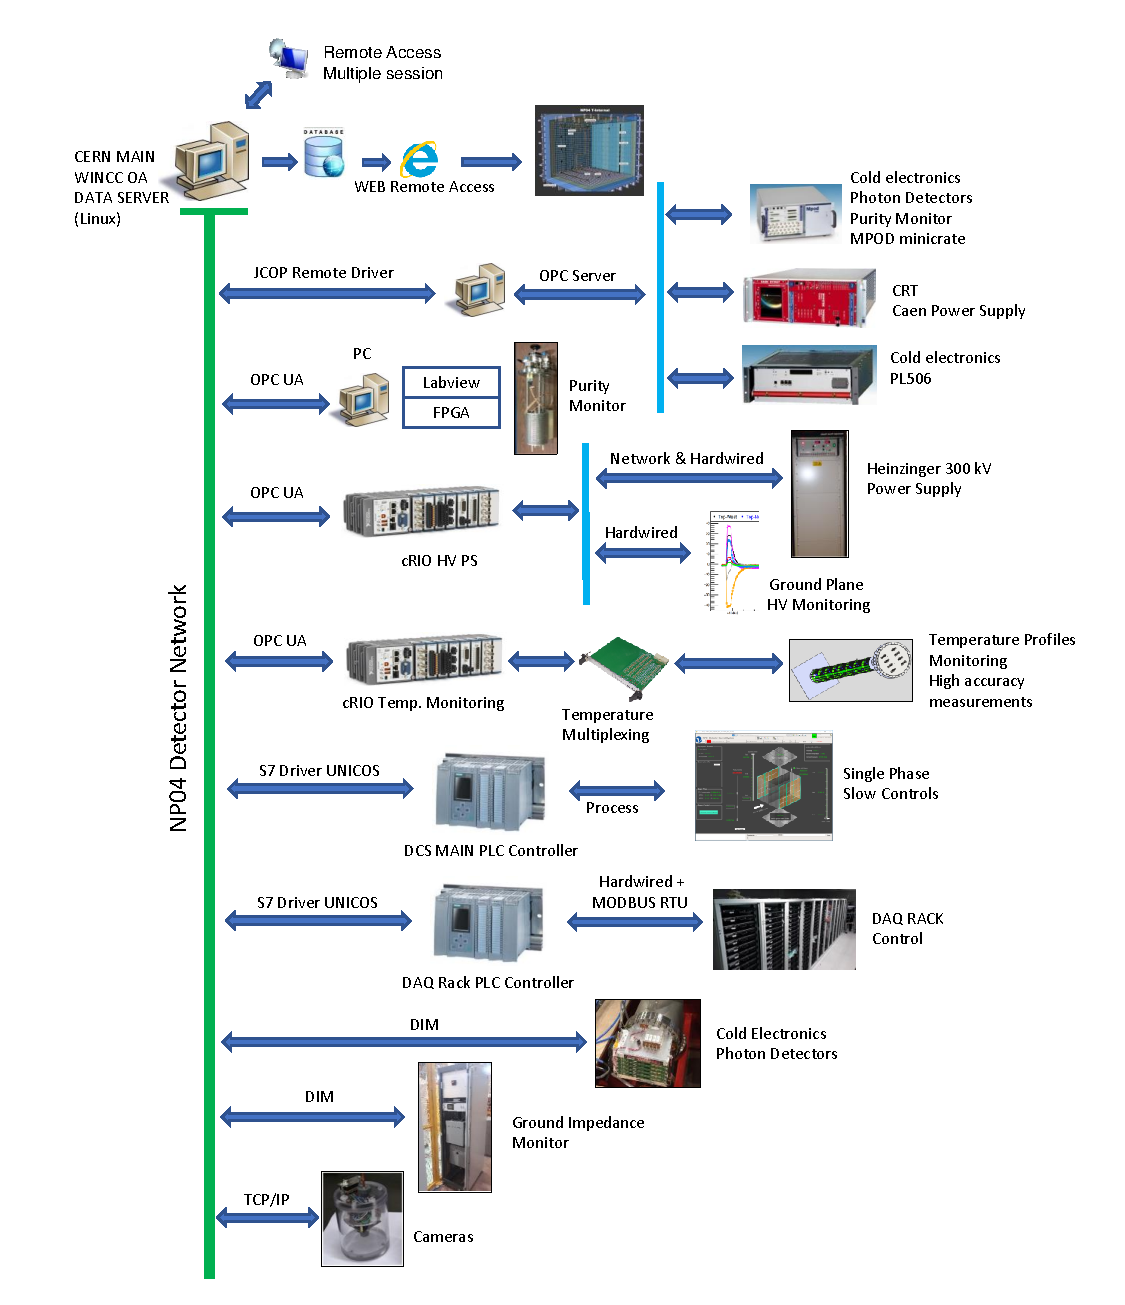
\includegraphics[height=0.9\textheight,width=0.95\textwidth,keepaspectratio]{NP04-DCS_arch_vert}
\end{dunefigure}

In this control system, the unified control system base is WinCC-OA~\cite{winccoa}, a commercial \dword{scada} system for visualizing and operating of processes, production flows, machines, and plants, used
in many businesses. It was chosen at \dword{cern} as a basis for
developing the control systems of the \dword{lhc} experiments, the
accelerators and the laboratory infrastructure for its flexibility and
scalability, as well as for the openness of the architecture, allowing
it to interface with many different types of hardware devices and
communication protocols. Additional software developed at \dword{cern}
is also used, including Joint COntrols Projects~\cite{jcop} and UNified
Industrial COntrol System (UNICOS)~\cite{unicos}.  WinCC-OA and the
additional software developed on top of it in the past 20 years, have
grown into a fairly complex ecosystem. While multiple collaboration
members have experience using the \dword{pdsp} control system,
customizing and using WinCC-OA in an effective way for developing the
control system of \dword{dune} requires proper training and a
non-negligible learning effort.


As noted in sections \ref{sec:fdgen-slow-cryo-sw} and \ref{sec:fdgen-slow-cryo-quant},
the slow control archiver will gradually accumulate terabytes of
data, requiring a sizable database to store the value history and
allow efficient data retrieval. Individually adjustable rates and
thresholds for each channel are key to keeping this database
manageable. The \dword{pdsp} operations provided not only a test of
these features as implemented in the \dword{protodune} slow control system, but also insight into
reasonable values for these archiving parameters for each system.


%%%%%%%%
\section{Organization and Management}
\label{sec:cisc-slow-controls-org}

%\fixme{SG/ACV:DONE}

The organization of the \dword{cisc} consortium is shown in
 Figure~\ref{fig:gen-slow-cryo-org}. The \dword{cisc} consortium board currently comprises institutional representatives from 19 institutes as shown in Table~\ref{tab:gen-slow-cryo-org}.  The consortium leader is the spokesperson for the consortium and responsible for the overall scientific program and managing the group. The technical leader of the consortium is responsible for managing the project for the group. Currently, the
consortium has five working groups:
\begin{description}
 \item[Cryogenics Systems:] gas analyzers and differential pressure liquid level
  monitors; \dword{cfd} simulations.
 \item[Argon Instrumentation:] purity monitors, thermometers (\dword{lar} and \dword{gar}), capacitive level meters, pressure meters (\dword{gar}), cameras and light emitting system, and \dword{citf}, also feedthroughs, \efield simulations, instrumentation precision studies, \dword{protodune} data analysis coordination and validation; 
 \item [Slow Controls Base Software and Databases:]  base I/O software, alarms and archiving databases, also monitoring tools,
   variable naming conventions, and slow controls quantities;
 \item [Slow Controls Detector System Interfaces:] signal processing software and hardware interfaces (e.g., power supplies), firmware, rack hardware, and infrastructure;   and 
 \item [Slow Controls External Interfaces:] interfaces with external detector systems (e.g., cryogenics system, beam, facilities, and \dword{daq}, near detector status).
\end{description}

\begin{dunefigure}[CISC consortium organization]{fig:gen-slow-cryo-org}
{CISC Consortium organizational chart.}
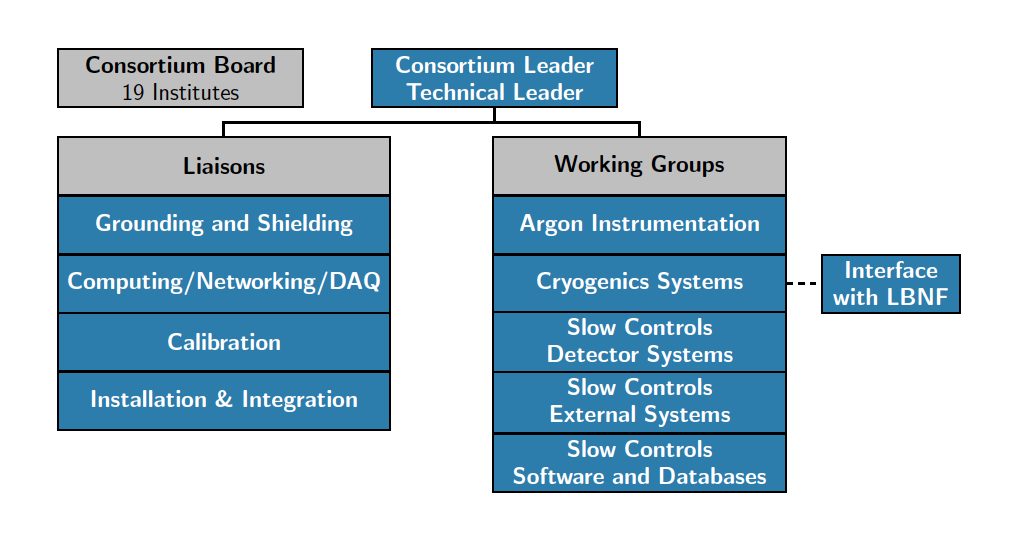
\includegraphics[width=0.8\textwidth]{graphics/cisc_org_20190716_zoomedin.png}
\end{dunefigure}

\begin{dunetable}
[CISC consortium institutions.]
%{p{0.43\textwidth}p{0.12\textwidth}p{0.22\textwidth}}
{lc}
{tab:gen-slow-cryo-org}
{Current \dword{cisc} Consortium Board Members and their institutional affiliations.}
Member Institute                         &  Country       \\%  &  Consortium Board Representative \\ \toprowrule
CIEMAT                                   &  Spain         %  &  Ines Gil Botella 
\\ \colhline
Instituto de Fisica Corpuscular (IFIC)          &  Spain          % &  Anselmo Cervera 
\\ \colhline
University of Warwick                    &  UK % &  Gary Barker 
\\ \colhline
University College London (UCL)             &  UK  %&  Mario Campanelli 
\\ \colhline
Argonne National Lab (ANL)                     &  USA             %&  Jim Grudzinski 
\\ \colhline
Brookhaven National Lab (BNL)                  &  USA            % &  Jim Stewart
\\ \colhline
University of California, Irvine (UCI)        &  USA            % &  Jianming Bian 
\\ \colhline
Drexel University                        &  USA           %  &  Charles Lane 
\\ \colhline
Fermi National Accelerator Lab (\fnal)           &  USA           %  &  Alan Hahn
\\ \colhline
University of Hawaii                     &  USA            % &  Jelena Maricic 
\\ \colhline
University of Houston                    &  USA           %  &  Andrew Renshaw 
\\ \colhline
Idaho State University (ISU)                   &  USA           %  &  Ed Tatar 
\\ \colhline
Kansas State University (KSU)                  &  USA            % &  Glenn Horton-Smith 
\\ \colhline
University of Minnesota, Duluth (UMD)         &  USA            % &  Alec Habig 
\\ \colhline
Notre Dame University                    &  USA            % &  John LoSecco 
\\ \colhline
South Dakota State University (SDSU)           &  USA            % &  Stephen Gent
\\ \colhline
University of Tennessee at Knoxville (UTK)     &  USA           %  &  Sowjanya Gollapinni 
\\ \colhline
Virginia Tech (VT)                            &	USA	           % &  Camillo Mariani
\\ \colhline
Boston University (BU)                        & USA %& Edward Kearns 
\\
\end{dunetable}

Moreover, because the \dword{cisc} consortium broadly interacts with other groups, liaisons have been named (see Figure~\ref{fig:gen-slow-cryo-org}). 
A short-term task force formed in 2017-2018 explored cryogenics modeling for the consortium and corresponding simulation needs. A work plan for \dword{cfd} simulations for both \dword{protodune} and \dword{fd} was developed based on input from the task force. 


\subsection{Institutional Responsibilities}
%\fixme{SG/ACV: DONE}
The \dword{cisc} %slow controls and cryogenic instrumentation 
will be a joint effort for \dword{sp} and \dword{dp}. %\single and \dual. 
A single slow controls system will be implemented to serve both the \dword{spmod} and the \dword{dpmod}.

Design and installation of cryogenics systems (e.g., gas analyzers, differential pressure liquid level meters) 
will be coordinated with \dword{lbnf} and the consortium providing resources and effort; expertise is provided by \dword{lbnf}. \dword{pdsp} and \dword{pddp} designs for argon instrumentation (e.g., purity monitors, pressure meters, thermometers, cameras) will be the basis for \dword{detmodule} designs. Design validation, testing, calibration, and performance will be evaluated using \dword{protodune} data.

Following the conceptual funding model envisioned for the consortium, various responsibilities have been distributed across institutions within the consortium pending final funding decisions.
Table~\ref{tab:cisc-inst-resp} shows the current institutional responsibilities for primary \dword{cisc} subsystems. Only lead institutes are listed in the table for a given effort. For physics and simulations studies and for validation using \dword{protodune}, a number of institutes are involved. A detailed list of tasks and institutional responsibilities are presented in~\cite{bib:docdb5609}.

\begin{dunetable}
[Institutional responsibilities in the CISC consortium ]
{p{0.4\textwidth}p{0.45\textwidth}}
{tab:cisc-inst-resp}
{Institutional responsibilities in the \dword{cisc} consortium.}
CISC Sub-system     &  Institutional Responsibility \\ \toprowrule
Purity monitors          &  UCI, Houston, UCL \\ \colhline
Static T-gradient monitors     &  IFIC, CIEMAT \\ \colhline
Dynamic T-gradient monitors & Hawaii \\ \colhline
Individual sensors & IFIC, CIEMAT \\ \colhline
Vertical thermometer arrays (GAr) & TBA \\ \colhline
Pressure meters (GAr) & TBA \\ \colhline
Readout system for thermometers & IFIC, Hawaii, CIEMAT \\ \colhline
Cold cameras & KSU, BNL \\ \colhline
Warm cameras & KSU, BNL \\ \colhline
Light-emitting system (for cameras) & Drexel \\ \colhline
Gas analyzers & FNAL, \dshort{lbnf} \\ \colhline
Differential pressure level meters & \dword{lbnf} \\ \colhline
Capacitive level meters & Notre Dame \\ \colhline
\dshort{citf} & FNAL, ANL \\ \colhline
\dshort{cfd} simulations & SDSU, ANL \\ \colhline
Other simulation \& validation studies & Number of Institutes \\ \colhline
Slow controls hardware & UMD, UTK, Drexel\\ \colhline
Slow controls infrastructure & UMD, UTK\\ \colhline
Slow controls base software & KSU, UTK, BU, Drexel, Warwick, UCL, ANL, IFIC\\ \colhline 
Slow controls signal processing & A number of institutes \\ \colhline
Slow controls external interfaces & VT, UTK, UMD \\
\end{dunetable}




\subsection{Schedule}
\label{sec:fdgen-cisc-schedule}

Table \ref{tab:dp-cisc-sched} shows key construction milestones for the \dword{cisc} consortium leading to commissioning of the second \dword{fd} module. \dword{cisc} construction milestones align with the overall construction milestones of the second \dword{fd} module (highlighted in orange in the table). The technology design decisions for \dword{cisc} systems should be made by April 2021 followed by final design reviews in June 2021. Design decisions will largely be based on how a given system performed (technically and physics-wise) in \dword{protodune}. This is currently actively ongoing with the \dword{pdsp} instrumentation data.  
As noted in section~\ref{sec:pddp-cryo-valid}, since the designs aimed for the \dual \dword{fd} are not deployed in the current run of \dword{pddp}, the plan is to test everything in the \dword{protodune2} \dword{dp} except for pressure meters and long capacitive level meters as they are already deployed in the current run of \dword{pddp}. The production of systems aimed for \dword{protodune2} \dual should be finished by January 2022 followed by assembly and deployment in March 2022. 

\begin{dunetable}
[DP CISC schedule]
{p{0.65\textwidth}p{0.25\textwidth}}
{tab:dp-cisc-sched}
{Key CISC construction schedule milestones leading to commissioning of the second FD module.}   
Milestone & Date (Month YYYY)   \\ \toprowrule
\rowcolor{dunepeach} Start of \dword{pdsp}-II installation& \startpduneiispinstall      \\ \colhline
Technology Decision Dates &   April 2021   \\ \colhline
Final Design Review Dates &   June 2021   \\ \colhline
Start of module 0 component production for ProtoDUNE-II & August 2021  \\ \colhline
End of module 0 component production for ProtoDUNE-II & January 2022  \\ \colhline
\rowcolor{dunepeach} Start of \dword{pddp}-II installation& \startpduneiidpinstall      \\ \colhline
\rowcolor{dunepeach}South Dakota Logistics Warehouse available& \sdlwavailable      \\ \colhline
\rowcolor{dunepeach}Beneficial occupancy of cavern 1 and \dword{cuc}& \cucbenocc      \\ \colhline
\rowcolor{dunepeach} \dword{cuc} counting room accessible& \accesscuccountrm      \\ \colhline
 \dword{prr} dates &  September 2023    \\ \colhline
Start procurement of \dword{cisc} hardware & December 2023 \\ \colhline

\rowcolor{dunepeach}Top of \dword{detmodule} \#1 cryostat accessible& \accesstopfirstcryo      \\ \colhline
Start of production of \dword{cisc} hardware & April 2024 \\ \colhline
\rowcolor{dunepeach}Start of \dword{detmodule} \#1 \dword{tpc} installation& \startfirsttpcinstall      \\ \colhline

\rowcolor{dunepeach}Top of \dword{detmodule} \#2 accessible& \accesstopsecondcryo      \\ \colhline
End of \dword{cisc} hardware production  &   April 2025   \\ \colhline

%Installation of gas analyzers & April 2025\\ \colhline
\rowcolor{dunepeach}End of \dword{detmodule} \#1 \dword{tpc} installation& \firsttpcinstallend      \\ \colhline
Start integration of \dword{cisc} hardware in the cavern & July 2025   \\ \colhline
 \rowcolor{dunepeach}Start of \dword{detmodule} \#2 \dword{tpc} installation& \startsecondtpcinstall      \\ \colhline
 Installation of gas analyzers and support structure for all instrumentation devices &  September 2025 \\ \colhline
Installation of individual sensors, static T-gradient thermometers, and level meters & November 2025\\ \colhline
All slow controls hardware, infrastructure, \& networking installed & February 2026\\ \colhline
Slow controls software for I/O, alarms, archiving, displays installed on production systems & May 2026 \\ \colhline
\rowcolor{dunepeach}End of \dword{detmodule} \#2 \dword{tpc} installation& \secondtpcinstallend      \\ \colhline
Install dynamic T-gradient monitors, cameras, purity monitors, and pressure meters & June 2026 \\\colhline
Install all feedthroughs for instrumentation devices & July 2026 \\ \colhline
Install slow control expert interfaces for all systems in time for testing & September 2026 \\ \colhline
Full slow controls systems commissioned and integrated into remote operations & July 2027 \\ 
\end{dunetable}



Designs may need review based on performance in \dword{protodune2} and any modifications will be incorporated into the final design before the start of production of \dword{cisc} systems for the \dword{fd} 
\fixme{\dword{dpmod}?} in April 2024. This will be followed by assembly of the systems underground in the detector cavern in July 2025. Installation of instrumentation devices will start in September 2025 following the beneficial occupancy of the interior of the cryostat. Installing gas analyzers, level meters, individual temperature sensors, static T-gradient thermometers, and support structure for all instrumentation devices will be finished before installing \dword{tpc}, but installation of dynamic T-gradient thermometers, purity monitors, pressure meters and cameras will occur afterward. \dword{cisc} will work closely with \dword{lbnf} to coordinate installation of the cryogenics systems and instrumentation devices. For slow controls, the goal is to have the full slow controls system commissioned and integrated into remote operations at least three months before the \dword{dpmod} is ready for operations.  




\subsection{Risks}


Table~\ref{tab:risks:DP-FD-CISC} lists the possible risks identified by the \dword{cisc} consortium along with corresponding mitigation strategies. 
A more detailed list of risks with additional descriptions can be found in \cite{bib:docdb7192}. The table shows 18 risks, all at medium or low level, mitigated with necessary steps and precautions. More discussion on all medium-level risks are provided in the text below. 
\begin{itemize}
    \item Risk 01: The risk associated with \dword{protodune}-based designs (mainly \dword{sp}) being inadequate for \dword{fd}, is important because this requires early validation from \dword{protodune} data so R\&D of alternate designs can be timely. With \dword{pdsp} data now available, the consortium is focused on validating instrumentation designs.
    \item Risk 06: Temperature sensors in the dynamic T-gradient monitor are calibrated using two methods: lab calibration to \SI{0.002}{K} (as in the static T-gradient monitor case) and in situ cross-calibration moving the system vertically. Disagreement between the two methods can occur. In order to mitigate this we need to investigate and improve both methods. 
    \item Risk 10: This risk involves an inability to build a working prototype for cold cameras during R\&D phase that meets all the requirements \& safety, e.g., that cold camera prototypes fail longevity tests or show low performance (e.g. bad resolution). This risk originates from past experience with cold cameras that became non-operational after a period of time in \dword{lar} or showed low performance. In order to address this, we plan to pursue further R\&D to improve thermal insulation and heaters, develop alternative camera models, etc. If problems persist one can use the cameras in the ullage (cold or inspection) with the appropriate field of view and lighting such that elements inside \dword{lar} can be inspected during filling.
    \item Risk 12: Cameras are delicate devices and some of them located near \dword{hv} devices can be destroyed by \dword{hv} discharges. This can be mitigated by ensuring that most important cold cameras have enough redundancy such that the loss of one camera does not compromise the overall performance. In the case of inspection cameras, % since they are replaceable, one 
    we can simply replace them.
    \item Risk 17: The gas analyzers and level meters may fail as these are commercial devices purchased at some point in their product cycle and cannot be required to last 20 years. Typical warranties are $\sim$1 year from date of purchase. The active electronics parts of both gas analyzers and level meters are external to the cryostat so they can be replaced. To mitigate this, provisions will be made for future replacement in case of failure or loss of sensitivity. Also, the risk is not high since we have purity monitors in the filtration system that can cover the experiment during the time gas analyzers are being replaced or repaired. 
\end{itemize}

Related to risks 12, 16 and 18, ageing is an important aspect for several monitors, especially for those that are inaccessible. The \dword{protodune} tests demonstrate that the devices survive the commissioning phase, and we continue to learn from \dword{protodune} experience. In addition to \dword{protodune}, other tests are planned. For example, in the case of purity monitors, photocathodes are expected to survive the first five years and if we prevent running them with high frequency at low purity (lifetime~$<$~\SI{3}{\milli\second}), ageing can be prevented for a longer time. To understand long-term ageing, R\&D is planned at \dword{citf} and at member institute sites for many of the devices. %Other s
Systems that are replaceable, such as inline purity monitors, gas analyzers, and inspection cameras, can be replaced when failures occur and maintained for the lifetime of the experiment.


% risk table values for subsystem DP-FD-CISC
\begin{footnotesize}
\begin{longtable}{p{0.18\textwidth}p{0.20\textwidth}p{0.32\textwidth}p{0.02\textwidth}p{0.02\textwidth}p{0.02\textwidth}}
%\begin{longtable}{x{0.18\textwidth}x{0.20\textwidth}x{0.32\textwidth}x{0.02\textwidth}x{0.02\textwidth}x{0.02\textwidth}} 
\caption{Risks for DP-FD-CISC (P=probability, C=cost, S=schedule) (more information at \dword{riskprob}). \fixmehl{ref \texttt{tab:risks:DP-FD-CISC}}} \\
\rowcolor{dunesky}
ID & Risk & Mitigation & P & C & S  \\  \colhline
RT-DP-CISC-001 & Baseline design from ProtoDUNEs for an instrumentation device is not adequate for DUNE far detectors & Focus on early problem discovery in ProtoDUNE so any needed redesigns can start as soon as possible. & L & M & L \\  \colhline
RT-DP-CISC-002 & Swinging of long instrumentation devices (T-gradient monitors or PrM system) & Add additional intermediate constraints to prevent swinging. & L & L & L \\  \colhline
RT-DP-CISC-003 & High E-fields near instrumentation devices cause dielectric breakdowns in \dword{lar} & CISC systems shielded and placed as far from cathode and FC as possible. & L & L & L \\  \colhline
RT-DP-CISC-004 & Light pollution from purity monitors and camera light emitting system & Use PrM lamp and camera lights outside PDS trigger window; cover PrM cathode to reduce light leakage. & L & L & L \\  \colhline
RT-DP-CISC-005 & Temperature sensors can induce noise in cold electronics & Check for noise before filling and remediate, repeat after filling. Filter or ground noisy sensors. & L & L  & L \\  \colhline
RT-DP-CISC-006 & Disagreement between lab and \em{in situ} calibrations for ProtoDUNE-SP dynamic T-gradient monitor & Investigate and improve both methods, particularly laboratory calibration. & M & L & L \\  \colhline
RT-DP-CISC-007 & Purity monitor electronics induce noise in TPC and PDS electronics. & Operate lamp outside TPC+PDS trigger window. Surround and ground light source with Faraday cage. & L & L & L \\  \colhline
RT-DP-CISC-008 & Discrepancies between measured temperature map and CFD simulations in ProtoDUNE-SP & Improve simulations with additional measurements inputs; use fraction of sensors to predict others   & L & L & L \\  \colhline
RT-DP-CISC-009 & Difficulty correlating purity and temperature in ProtoDUNE-SP impairs understanding cryo system. & Identify causes of discrepancy, modify design. Calibrate PrM differences, correlate with RTDs. & L & L & L \\  \colhline
RT-DP-CISC-010 & Cold camera R\&D fails to produce prototype meeting specifications \& safety requirements & Improve insulation and heaters. Use cameras in ullage or inspection cameras instead. & M & M & L \\  \colhline
RT-DP-CISC-011 & HV discharge caused by inspection cameras & Study E-field in and on housing and anchoring system. Test in HV facility. & L & L & L \\  \colhline
RT-DP-CISC-012 & HV discharge destroying the cameras & Ensure sufficient redundancy of cold cameras. Warm cameras are replaceable. & L & M & L \\  \colhline
RT-DP-CISC-013 & Insufficient light for cameras to acquire useful images & Test cameras with illumination similar to actual detector. & L & L & L \\  \colhline
RT-DP-CISC-014 & Cameras may induce noise in cold electronics & Continued R\&D work with grounding and shielding in realistic conditions. & L & L & L \\  \colhline
RT-DP-CISC-015 & Light attenuation in long optic fibers for purity monitors  & Test the max.\ length of usable fiber, optimize the depth of bottom PrM, number of fibers. & L & L & L \\  \colhline
RT-DP-CISC-016 & Longevity of purity monitors & Optimize PrM operation to avoid long running in low purity. Technique to protect/recover cathode. & L & L & L \\  \colhline
RT-DP-CISC-017 & Longevity: Gas analyzers and level meters may fail. & Plan for future replacement in case of failure or loss of sensitivity.  & M & M & L \\  \colhline
RT-DP-CISC-018 & Problems in interfacing  hardware devices (e.g. power supplies) with slow controls & Involve slow control experts in choice of hardware needing control/monitoring.
 & L & L & L \\  \colhline

\label{tab:risks:DP-FD-CISC}
\end{longtable}
\end{footnotesize}


\subsection{Interfaces}  
\label{sec:interfaces}

\dword{cisc} subsystems interface with all other detector subsystems and could affect the work of all detector consortia, as well as some
working groups (e.g., physics, software and computing, beam instrumentation), and technical coordination, requiring interactions with all of these entities.  We also interact heavily with \dword{lbnf} beam and cryogenics groups.  
Detailed descriptions of \dword{cisc} interfaces are maintained in \dword{dune} DocDB. A brief summary is provided in this section. Table~\ref{tab:fdgen-cisc-interfaces} lists the IDs of the different DocDB documents as well as their highlights. Descriptions of the interfaces and interactions that affect many systems follow. 

%Obviously,
 \dword{cisc} interacts with the detector consortia because \dword{cisc} will provide status monitoring of all important detector subsystems along with controls for some components of the detector.
\dword{cisc} will also consult on selecting different power supplies to ensure monitoring and control can be established with preferred types of communication. 
Rack space distribution and interaction between slow controls and other modules from other consortia will be managed by \dword{tc} in consultation with those consortia. 

If heaters/\dwords{rtd} are needed on flanges, \dword{cisc} will specify the heaters/\dwords{rtd} and will provide the readout/control, while the responsibility for the actual hardware will be discussed with the different groups.  

Installing instrumentation devices will interfere with other devices and must be coordinated with the appropriate consortia.  
On the software side, \dword{cisc} must define, in coordination with other consortia/groups, the quantities to be monitored/controlled by slow controls and the corresponding alarms,
archiving, and GUIs. 



%\fixme{reduced the text in the description column so that we don't have to move to longtable format. anne}
\begin{dunetable}
[CISC system interface links]
{p{0.15\textwidth}p{0.45\textwidth}p{0.14\textwidth}}
{tab:fdgen-cisc-interfaces}
{\dword{cisc} system interface links.}   % These are called Interface Documents in Doc-DB, also in Work Breakdown Structure documents.
\small
Interfacing System & Description & Linked Reference \\ \toprowrule
%test & & \citedocdb{6628} \\ \colhline
\dword{crp}	           &
               
temperature sensors in the gas, cameras, and lights
& \citedocdb{6760} 
\\ \colhline

\dword{pds}	     & 

PrMs, light emitting system for cameras
& \citedocdb{6781}  
\\ \colhline

\dword{tpc} Electronics	         &  
noise, power supply monitoring
& \citedocdb{6784}  \\ \colhline


\dword{hv} Systems	           &

shielding, bubble generation by inspection camera, cold camera locations, ground planes
& \citedocdb{6787}   
\\ \colhline

\dword{daq}	                      &
description of \dword{cisc} data storage, 
allowing bi-directional communications between \dword{daq} and \dword{cisc}.      & \citedocdb{6790}
\\ \colhline
Calibration          &

multifunctional \dword{cisc}/\dword{citf} ports; space sharing around ports 
& \citedocdb{7072} 

\\ \colhline
Physics	          &

indirect interfaces through calibration, tools to extract data from the slow controls database %& \citedocdb{7099} 
\\ \colhline

Software \& Computing	  &

slow controls database design and maintenance
& \citedocdb{7126}  
\\ \colhline

Cryogenics             &  

must be designed and implemented.       
purity monitors, gas analyzers, interlock mechanisms to prevent contamination of LAr
&  -   

\\ \colhline

Beam                      &   %At least the status of this system will be monitored  
beam status &  -     
\\ \colhline
TC Facility              &   
significant interfaces at multiple levels   
& \citedocdb{6991}   \\ \colhline
TC Installation     	  &     
significant interfaces at multiple levels
& \citedocdb{7018}   \\ \colhline
TC Integration Facility    &    
significant interfaces at multiple levels
& \citedocdb{7045}   \\ 
\end{dunetable}






\subsection{Installation, Integration, and Commissioning}

%\fixme{SG (04/15): pressure meters are missing here}
\subsubsection{Purity Monitors}
\label{sec:fdgen-slow-cryo-install-pm}


The purity monitor system will be built in modules, so it can be assembled outside the %\dword{dune} \dword{fd} 
cryostat  
leaving few steps to complete inside the cryostat.  The assembly itself %should
 comes into the cryostat with the individual purity monitors mounted to support tubes and with no \dword{hv} cables or optical fibers yet installed.  The support tube at the top and bottom of the assembly %would then be 
 is then mounted to the brackets inside the cryostat and  %; the brackets could be 
 the brackets attached to the cables trays and/or the detector support structure.  At much the same time, the \dword{fe} electronics and light source can be installed on top of the cryostat, and the electronics and power supplies can be installed in the electronics rack.  

Integration %would 
begins by running the  \dword{hv} cables and optical fibers to the purity monitors through the top of the cryostat.  These cables %would be 
are attached to the  \dword{hv}  feedthroughs with sufficient length to reach each purity monitor inside the cryostat.  
The cables %would be 
are run along cable trays through the port reserved for the purity monitor system. 
Each purity monitor will have three  \dword{hv} cables that connect it to the feedthrough and then further along to the  \dword{fe} electronics.  The optical fibers %would then be 
are then run through the special optical fiber feedthrough into the cryostat and %would be 
guided to the purity monitor system either using the cables trays or guide tubes, depending on which solution is adopted. 
%for running the optical fibers from the feedthrough to the purity monitor system, 
This should protect fibers from breaking accidentally as the rest of the detector and instrumentation installation continues.  The optical fibers %would then be 
are then run inside the purity monitor support tube and to the appropriate purity monitor, terminating the fibers at the photocathode of each monitor while protecting them from breaking near the purity monitor system itself.

Integration %would 
continues as the  \dword{hv} cables are connected through the feedthrough to the system  \dword{fe} electronics; then optical fibers are connected to the light source.  The cables connecting the \dword{fe} electronics and the light source to the electronics rack %would also be 
are also run and connected at this time.  This allows the system to be turned on and the software to begin testing the various components and connections.  Once all connections are confirmed successful, integration with the slow controls system begins, first by establishing communication between the two systems and then transferring data between them to ensure successful exchange of important system parameters and measurements.  

Commissioning the purity monitor system % is considered  official
begins once the cryostat is purged and a gaseous argon atmosphere is present.  At this time, the \dword{hv} for the purity monitors 
  is ramped up without risk of discharge through the air, and the light source turned on.  Although the drift electron lifetime in the gaseous argon would be very large and therefore not %really 
  measurable with the purity monitors themselves, the signal strength at both the cathode and anode will %would 
  give a good indication of how well the light source generates drift electrons from the photocathode. % and  that the electrons successfully drift to the anode by looking at the signal strength at the anode and comparing it to the cathode signal strength.
  Comparing the signal strengths at the anode and cathode will indicate whether the electrons successfully drift to the anode.
  Although \dword{qa} and \dword{qc} should make it unlikely for a purity monitor to fail this final test, if that does happen then the electric and optical connections can be fixed before filling.

\subsubsection{Thermometers}
\label{sec:fdgen-slow-cryo-install-th}

\paragraph{Static T-gradient monitors}
 %should 
are installed after \dwords{fc} along the long cryostat sides. The profiles %will be 
are preassembled before they are delivered to \surf. 
Installation begins by anchoring the support holding the two vertical strings to bolts on the top corner of the cryostat. All cables can then be routed to the assigned cryostat ports. Second, the array is unrolled using a scissor lift, and once at the bottom, it is attached to bolts on the bottom corner of the cryostat. After checking string tension and verticality, cable and sensors supports are checked, and the individual Faraday cages are installed. A precision resistor is plugged into each IDC-4 connector, so noise studies can be performed. Sensors will be installed later. 

\paragraph{Individual temperature sensors} on pipes/\dwords{pd}\footnote{Actually on \dshort{pd}'s support structure}  and cryostat floor %will be 
should be installed after \dwords{pd} and the grounding grid. First, vertical strings for cable routing %will be 
are installed following a procedure similar to the one described above for the static T-gradient monitors. Next, anchor all cable supports to pipes/\dshorts{pd}. Then each cable %will be 
is routed individually starting from the sensor end (with IDC-4 female connector but without the sensor)
to the corresponding cryostat port. Once all cables going through the same port have been routed, the cables are cut to the same length, so they can be properly assembled into the corresponding connector(s). To avoid damaging them, sensors are installed later, once all operations at the bottom of the cryostat are complete. 

 


\paragraph{Dynamic T-gradient monitors} %will be 
are installed
after the \dword{tpc} components are in place.
Figure~\ref{fig:fd-slow-cryo-dt-monitor-overview} shows the
design of the dynamic T-gradient monitor with its sensor carrier rod,
enclosure above the cryostat, and stepper motor. 
 Figure~\ref{fig:fd-slow-cryo-sensor-mount} shows detailed views of key
components.  Each monitor %will 
comes in several segments with sensors
and cabling already in place. Additional slack will be provided at
segment joints to make installation easier. Segments of the sensor
carrier rod with preattached sensors %will be 
are fed into the flange one
at a time. Each segment, as it is fed into the %detector
cryostat, is % will be
held at the top with a pin that prevents the segment from sliding all
the way in. %to the detector. 
The next segment %will be 
is connected at that
time to the previous segment. Then the pin %will be 
is removed, the first
segment %will be 
is pushed down, and the next segment top %will be 
is held
with the pin at the flange. This process %will be 
is repeated for each
segment %to be installed 
until the entire sensor carrier rod is in
place.  Next, the enclosure %will be 
is installed on top of the flange,
starting with the six-way cross at the bottom of the enclosure.  (See
 Figure~\ref{fig:fd-slow-cryo-sensor-mount}, right.)  Again, extra cable
slack at the top will be provided to ease connection to the D-sub
flange and allow the entire system to move vertically.  The wires
%will be 
are connected to a D-sub connector on the \fdth on one side port
of the cross. Finally, a crane %will be used to 
positions the remainder
of the enclosure over the top of the cross.  This enclosure includes
the mechanism used to move the sensor rod, which %will be 
is preassembled,
with the motor in place, on the side of the enclosure, and the pinion
and gear is used to move the sensor inside the enclosure.  The pinion
%will be 
is connected to the top of the rod. The enclosure is then %will then be
connected to top part of the cross, which finishes the installation of
the dynamic T-gradient monitor.


\paragraph{Vertical arrays in gas phase:} The baseline design assumes 20 arrays, each of which is attached to a \dword{crp} frame. Thus, they should be installed on the corresponding \dword{crp} before being moved into the cryostat. Cables will be routed to the assigned cryostat port using the appropriate elements on the \dword{crp} frame. 

Commissioning all thermometers will occur in several steps. In the first stage, only cables %will be 
are installed, so
the readout performance and the noise level inside the cryostat %will be
is checked again at room temperature.
Spare cables, connectors and sensors are available for replacement at \dword{surf} if needed. 
The final commissioning phase %will be done
takes place during and after cryostat filling.  


\subsubsection{Gas Analyzers}
\label{sec:fdgen-slow-cryo-install-ga}
%\fixme{IIC Gas Analyzers: To be reviewed}

%\fixme{AC: VALID SUBSECTION}

The gas analyzers %should be 
are installed before the piston purge and gas recirculation phases of the cryostat commissioning. They %should be 
are installed near the tubing switchyard to minimize tubing run length and for convenience when switching the sampling points and gas analyzers. Because each is a standalone module, a single rack with shelves %should be 
is adequate to house the modules.

For integration, the gas analyzers typically have an analog output (\SIrange{4}{20}{mA} or \SIrange{0}{10}{V}), which maps to the input range of the analyzers. They also usually have several relays to indicate the scale they are currently running. These outputs can be connected to the slow controls for readout. However, using a digital readout is preferable because this gives a direct analyzer reading at any scale. Currently, the digital output connections are RS-232, RS-485, USB, and Ethernet. The preferred option is chosen at the time of purchase. %When they are purchased, the preferred option can be chosen, but the available protocols for the modules may change. 

The readout usually responds to a simple set of text query commands. Because of the natural time scales of the gas analyzers and lags in gas delivery times (which depend on the length of the tubing run), sampling every minute is adequate.

The analyzers %should 
must be brought online and calibrated before beginning the gas phase of the cryostat commissioning.  Calibration varies by module because they differ, but calibration often requires using argon gas with zero contaminants, and argon gas with a known level of the contaminant to check the scale. Contaminants are usually removed with a local inline filter for the first gas sample. %The gas phase of the cryostat 
This gas phase usually begins with normal air, with the more sensitive analyzers valved off at the switchyard to prevent overloading their inputs (and potentially saturating their detectors). As the argon purge and gas recirculation progress, the various analyzers %will be 
are valved back in when the contaminant levels reach the upper limits of the analyzer ranges. 

\subsubsection{Liquid Level Monitoring}
\label{sec:fdgen-slow-cryo-install-llm}

%\fixme{AC: DONE. Slightly modified}

\dword{lbnf} will install differential pressure level meters, but the capacitive level meters fall within scope of \dword{cisc}. The exact number of capacitive level meters is not yet decided. We will need at least four, one for each of the four corners of the cryostat.  
They will be attached to the M10 bolts in the cryostat corners after the detector is installed. If additional capacitive level meters are needed in the central part of the cryostat, those will be installed after the nearby \dword{fc} modules, attaching them to the bolts in the top cryostat corner\footnote{These level meters must be shorter because no bolts run vertically as they do for the other level meters}. In all cases, cables will be routed to the appropriate nearby port (not yet assigned). 

\subsubsection{Pressure Meters}
\label{sec:fdgen-slow-cryo-install-press}
%\fixme{SG: to be reviewed by experts}
\dword{cisc} will install the pressure meters. Six sensors will be mechanically installed in two dedicated flanges (three sensors each) at opposite sides of the cryostat after the detector is installed. Cables will be routed through the dedicated ports assigned for these devices. The pressure signals (absolute and relative) are read and converted to
%electrical signals corresponding to 4...20~mA range.
standard 4--20 mA current loop signals.
A twisted pair shielded cable connects the sensors to the slow controls \dword{plc} controller using software to convert electrical signals to pressure values.

\subsubsection{Cameras and light emitting system}
\label{sec:fdgen-slow-cryo-install-c}
%\fixme{IIC Cameras: To be reviewed}

%\fixme{Reviewed by Glenn, updated light source installation. Done.}

Installing fixed cameras is, in principle, simple but involves several interfaces. The enclosure of each camera has
exterior threaded holes for mounting the cameras on the cryostat wall,
cryogenic internal piping, or \dword{dss}. Each
enclosure %will be 
is attached to a gas line to maintain appropriate
underpressure in the fill gas; %and so 
therefore, an interface with cryogenic
internal piping will be necessary. Each camera has a cable (coaxial or
optical) for the video signal and a multiconductor cable for power and
control. These %will be 
are run through cable trays to flanges on assigned
instrumentation feedthroughs.

The inspection camera is designed to be inserted and removed on any
instrumentation feedthrough equipped with a gate valve at any time
during operation.  Installing the gate valves and purge system
for instrumentation feedthroughs falls under cryogenic internal
piping.

Fixed lighting sources separate from the cameras
are mounted on cryostat wall, cryogenic internal piping, or
\dword{dss}, and multiconductor cables for power are run through cable
trays to flanges on assigned instrumentation feedthroughs.



\subsubsection{Slow Controls Hardware}
\label{sec:fdgen-slow-cryo-install-sc-hard}
%\fixme{IIC Slow Controls Hardware: To be reviewed}

Slow controls hardware installation %will 
includes several
servers, network cables, any specialized cables needed
for device communication, and possibly some custom-built hardware for monitoring racks. The installation sequence will be 
planned with the facilities group and other consortia. The network
cables and rack monitoring hardware will be common across many racks
and will be installed first as part of the basic rack installation as %which will 
led by the facilities group. Specialized cables needed for slow controls and servers %will be 
are installed
after the common rack hardware. Selecting and installing these cables will be coordinated
with other consortia, and server installation will be coordinated with the \dword{daq} group.

\subsubsection{Transport, handling, and storage}
\label{sec:fdgen-slow-cryo-install-transport}


Most instrumentation devices will be shipped in pieces to \surf via the \dword{sdwf} and mounted on site. 
Instrumentation devices are in general small, except for
the support structures for purity monitors and dynamic T-gradient monitors
that will cover the entire height of the cryostat. The load on those structures is relatively small (\(<\SI{100}{kg}\)), so they can be fabricated in sections smaller than \SI{3}{m},
which can be easily transported to \surf, down the shaft, and through the tunnels.
All instrumention devices except the dynamic T-gradient monitors can be moved into the cryostat without the crane. The dynamic T-gradient monitors, which %will be 
are introduced into the cryostat from above, %will 
require a crane for installing  the external enclosure (with preassembled motor, pinion, and gear). % on top of the cryostat. 


\subsection{Quality Control}
\label{sec:fdsp-slow-cryo-qc}
%\fixme{CP: Reviewed. Minor modifications and fixmes added. ACV: checked --> OK}
%\fixme{SG (4/15): pressure meters missing under QC}
The manufacturer and the institution in charge of device assembly will conduct a series of tests to ensure the equipment can perform its intended function as part of \dword{qc}. \dword{qc} also includes post-fabrication tests and tests run after shipping and installation. For complex systems, the entire system will be tested before shipping. 
Additional \dword{qc} procedures can be performed at the \dword{citf} and underground after installation. % as much as possible. 

The planned tests for each subsystem are described below.  

%\fixme{QC: To be reviewed}

\subsubsection{Purity monitors}
\label{sec:fdgen-slow-cryo-qc-pm}


The purity monitor system will undergo a series of tests to ensure the
system performs as intended. These tests 
%reflect the \dword{pdsp} purity monitor QC tests, which included
include electronic tests
with a pulse generator, mechanical and electrical connectivity tests
at cryogenic temperatures in a cryostat, and vacuum tests for short
and full assemblies in a dewar and in a long vacuum tube.

The \dword{qc} tests for \dword{fd} purity monitors begin with testing
individual purity monitors in vacuum after each is fabricated and
assembled.  This test checks the amplitude of the signal generated by
the drift electrons at the cathode and anode to ensure the
photocathode can provide sufficient numbers of photoelectrons to
measure the signal attenuation
with the required precision and the field gradient resistors all work properly to maintain the drift field. %and hence transport the drift electrons to the anode.  
A smaller version of the assembly with all purity monitors installed will be tested at the \dword{citf}
%in the \lar test facility 
to ensure the full system performs as expected in \dword{lar} and to study systematics that may influence the measured lifetime.

Next, %after individual testing would be 
the entire system %will be 
is assembled on the full-length mounting tubes to check connections.  Ensuring that all electric and optical connections are operating properly during this test reduces the risk of problems once the full system is assembled and ready for the final test in vacuum.  %With the full system assembled it would be 
The fully assembled system %can be 
is placed in the shipping tube, which %can 
serves as a vacuum chamber, and tested at \surf %on the \dword{fd} site
 before the system is inserted into the  %\dword{fd}  
 cryostat. During insertion, electrical connections %will be 
 are tested continuously with multimeters and electrometers. 


\subsubsection{Thermometers}
\label{sec:fdgen-slow-cryo-qc-th}

\paragraph{Static T-gradient thermometers:}
\label{sec:fdgen-slow-cryo-qc-thst}

Static T-gradient monitors undergo three type of tests at the production site before %they are shipped 
shipping to \surf: a mechanical rigidity test, a calibration of all sensors, and a test of all electrical cables and connectors.
Mechanical rigidity is tested by installing the static T-gradient monitor between two dummy cryostat corners mounted \SI{15}{m} apart. The tension of the strings is set to match the tension that would occur in a vertical deployment in \lar, and the deflection of the sensor and electrical cable strings is measured and compared to the expected value; this ensures any swinging or deflection of the deployed static T-gradient monitor will be < \SI{5}{cm}, mitigating any risk of touching the \dwords{fc} and the cryostat membrane.
The laboratory calibration of sensors will be performed 
as explained in Section~\ref{sec:fddp-cryo-therm}. The main concern is reproducibility of results because sensors could change resistance and hence their temperature scale when undergoing successive immersions in \lar. In this case, the calibration procedure itself provides \dword{qc} because each set of sensors goes through five independent measurements. Sensors with \rms variation outside the requirement (\SI{2}{mK} for \dword{pdsp}) are discarded. This calibration also serves as \dword{qc} for the readout system (similar to the final one) and of the \dword{pcb}-sensor-connector assembly.
Finally, the cable-connector assemblies are tested; sensors must measure the expected values with no additional noise introduced by either cable or connector. 

An integrated system test at a \dword{lar} test facility on site, with sufficient linear dimension (>\SI{2}{m}) to test a good portion of the system, would be desirable. This would ensure that the system
operates in \lar at the required performance level. \fixme{sp says test will be conducted at production site and compared with in situ. anne}

The last phase of \dword{qc} takes place after installation. The verticality of each array %will be 
is checked, and the tensions in the stainless steel strings adjusted as necessary.
Before closing the flange, the entire readout chain is %will be 
tested.  
This allows a test of the sensor-connector assembly, the cable-connector assemblies at both ends, and the noise level inside the cryostat.
If any sensor presents a problem, it is replaced. If the problem persists, the cable is checked and replaced as needed.

\paragraph{Dynamic T-gradient thermometers:}
\label{sec:fdgen-slow-cryo-qc-thdy}

The dynamic T-gradient monitor consists of an array of high-precision temperature sensors mounted on a vertical rod. The rod can move vertically to cross-calibrate the temperature sensors in situ. %{\em in situ}. 
We will use the following %several 
tests to ensure that the dynamic T-gradient monitor delivers vertical temperature gradient measurements with a precision of a few \si{mK}.

\begin{itemize}
\item
Before installation, temperature sensors are tested in \dword{ln} 
to verify correct operation and to set the baseline calibration for each sensor to the absolutely calibrated reference sensor. 
\item
Warm and cold temperature readings are taken with each sensor after it is mounted on the \dword{pcb} board and the readout cables are soldered. %of .
\item
The sensor readout is taken for all sensors after the cold cables are connected to electric \fdth{}s on the flange and the warm cables outside of the cryostat are connected to the temperature readout system.
\item 
The stepper motor is tested before and after connecting to the gear and pinion system.
\item
The fully assembled rod is connected to the pinion and gear and moved with the stepper motor on a high platform many times to verify repeatability, possible offsets, and any uncertainty in positioning. Finally, repeating this test many times will verify the sturdiness of the system.
\item
The full system is tested after it is installed in the cryostat; both motion and sensor operation are tested by checking % readout for sensors and motion of the system vertically. 
sensor readout and vertical motion of the system.
\end{itemize} 

\paragraph{Individual sensors:}
\label{sec:fdgen-slow-cryo-qc-is}

To address the quality of individual precision sensors, the same method is used as for the static T-gradient monitors %will be 
is used.
The \dword{qc} of the sensors is part of the laboratory calibration. After mounting six sensors with their corresponding cables, a
SUBD-25 connector %will be 
is added, and the six sensors tested at room temperature. All sensors %should 
must %work and 
give values within specifications.  
If any of the sensors present problems, they are replaced.  If the problem persists, the cable is checked and replaced as needed.

For standard \dwords{rtd} to be installed on the cryostat walls, floor, and roof, calibration is not an issue. Any \dword{qc} required for associated cables and connectors %will be 
is performed following the same procedure as for precision sensors. 


\paragraph{Vertical arrays in gas phase:}
\label{sec:fdgen-slow-cryo-qc-gs}

These thermometers use standard \dwords{rtd} that require no calibration.  Any \dword{qc} required for associated cables and connectors is performed following the same procedure as for precision sensors. The appropriate \dword{qc} procedure for the \dword{pcb} support structure will be elaborated once this is designed.  


\subsubsection{Gas analyzers}
\label{sec:fdgen-slow-cryo-qc-ga}


The gas analyzers will be guaranteed by the manufacturer. However, once received, the gas analyzer modules %will be 
are checked for both \textit{zero} and the \textit{span} values using a gas-mixing instrument and two gas cylinders, one having a zero level of the gas analyzer contaminant species and the other cylinder with a known percentage of the contaminant gas. This %should
 verifies the proper operation of the gas analyzers. When they are installed at \surf, this process %will be 
 is repeated before commissioning the cryostat. Calibrations must be repeated %at times recommended by the 
 using manufacturer recommendations over the gas analyzer lifetime.


\subsubsection{Liquid level monitoring}
\label{sec:fdgen-slow-cryo-qc-llm}

The manufacturer will provide the \dword{qc} for the differential pressure level meters; further \dword{qc} during and after installation %will be 
is the responsibility of \dword{lbnf}.

The capacitive sensors will be tested with a modest sample of \lar in the laboratory before they are installed. After installation, they are tested in situ %{\em in situ} 
using a suitable dielectric in contact with the sensor.

\subsubsection{Pressure meters}
\label{sec:fdgen-slow-cryo-qc-press}
%\fixme{SG: to be reviewed by experts}
The manufacturer will provide the \dword{qc} for the pressure meters; \dword{cisc} will provide further \dword{qc} during and after installation.

The pressure sensors will be tested with a modest sample of gaseous argon in the laboratory before they are installed. After installation, they are tested in situ at atmospheric pressure. The whole pressure readout chain, (including slow controls \dword{plc} and software protocol) 
%WINCC conversion) 
will also be tested and cross-checked with \dword{lbnf} pressure sensors.

\subsubsection{Cameras}
\label{sec:fdgen-slow-cryo-qc-c}

Before %being 
transport to \surf, each cryogenic camera unit (comprising the enclosure, camera, and internal thermal control and monitoring) %will be 
is checked for correct operation of all features, for recovery from \SI{87}{K} non-operating mode, for leakage, and for physical defects. Lighting systems %will be 
are similarly checked. Operations tests will verify correct current draw, image quality, and temperature readback and control. Each movable inspection camera apparatus %will be 
is inspected for physical defects and checked for proper mechanical operation before shipping. A checklist %will be 
is created for each unit, filed electronically in the \dword{dune} logbook, and a hard copy is sent with each unit. 

Before installation, each fixed cryogenic camera unit is inspected for physical damage or defects and checked at the \dword{citf} 
%in a cryogenics test facility  
for correct operation of all features, for recovery from \SI{87}{K} non-operating mode, and for contamination of the \dword{lar}. Lighting systems are similarly checked. Operations tests verify correct current draw, image quality, and temperature readback and control. After installing and connecting the wiring, fixed cameras and lighting are again  checked for operation. The movable inspection camera apparatus is inspected for physical defects and, after integration with a camera unit, tested in the facility for proper mechanical and electronic operation and cleanliness before being installed or stored. A checklist will be completed for each \dword{qc} check and filed electronically in the \dword{dune} logbook. 

\subsubsection{Light-emitting system}
\label{sec:fdgen-slow-cryo-qc-les}

The entire light-emitting system is checked before installation to ensure functionality of light emission. 
Initial testing of the system (see Figure~\ref{fig:cisc-LED}) begins with
measuring the current when low voltage (\SI{1}{V}) is applied to check
that the resistive \dword{led} failover path is correct. Next, the forward voltage is measured using nominal forward current to
check that it is within \SI{10}{\%} of the nominal forward voltage drop of
the \dword{led}, that all of the \dwords{led} are illuminated, and that each \dword{led} is visible over the nominal angular range. If the \dwords{led} are
infrared, a video camera with the IR filter removed is used for a
visual check. This procedure is then duplicated with the current
reversed for \dwords{led} oriented in the opposite direction. Initial tests are performed at room temperature and then repeated in \dword{ln}. 
Color shifts in the \dwords{led} are expected and will be noted. A checklist is completed for each \dword{qc} check and filed electronically in the \dword{dune} logbook.

Room temperature tests are repeated during and immediately after installation to ensure that the system has not been damaged during transportation or installation. Functionality checks of the \dwords{led} are repeated after the cameras are installed in the cryostat.

\subsubsection{Slow controls hardware}
\label{sec:fdsp-slow-cryo-qc-sc-hard}

Networking and computing systems will be purchased commercially, requiring manufacturer's\dword{qa}. The new servers %will be 
are tested after delivery to confirm they suffered no damage during shipping. The new system is allowed to burn in overnight or for a few days, 
running a diagnostics suite on a loop to validate %. This should turn up anything that escaped 
the manufacturer's \dword{qa} process.

The system %can be 
is shipped directly to \surf
where an on site
expert %will 
boots the systems and does basic
configuration. %Then s
Specific configuration information %will be 
is pulled over
the network, after which others may log in remotely to do the final
set up, minimizing the number of people underground.


\subsection{Safety}
Safety %should be taken into account 
is critical during %the different 
all phases of the \dword{cisc} project, including R\&D, laboratory calibration and testing, mounting tests, and installation. 
Safety experts %will 
review and approve the initial safety planning for all phases as part of the initial design review, as well as %always 
before implementation. 
All documentation of component cleaning, assembly, testing, and installation will include a section on relevant safety concerns and will be reviewed during appropriate pre-production reviews.

Several areas are of particular importance to \dword{cisc}.
\begin{itemize}
\item Hazardous chemicals (e.g., epoxy compounds used to attach sensors to cryostat inner membrane) and cleaning compounds:
  All chemicals used will be documented at the consortium management level, with a material safety data sheet
  and approved handling and disposal plans in place.

\item Liquid and gaseous cryogens used in calibrating and testing: \dword{ln} and \dword{lar} %will be 
are used to calibrate and test instrumentation devices.
  Full hazard analysis plans will be in place at the consortium management level for full module or
  module component testing that involves %cryogenic hazards. 
  cryogens. These safety plans will be reviewed in appropriate pre-production and production reviews.

\item High voltage safety:  Purity monitors %will 
have a voltage of $\sim\,$\SI{2}{kV}. Fabrication and testing plans will show compliance with local
  \dword{hv} safety requirements at %whichever 
  any institution or laboratory that conducts testing or operation, and this compliance will be reviewed as part of the standard review process.

\item Working at heights: Some fabrication, testing, and installation of \dword{cisc} devices require working at heights.
  Both T-gradient monitors and purity monitors, which span the height of the detector, require working at heights exceeding \SI{10}{m}.
  Temperature sensors installed near the top cryostat membrane and cable routing for all instrumentation devices
  %will 
  also require working at heights. % as well. 
  The appropriate safety procedures, including lift and harness training, will be designed and reviewed. 
  
\item Falling objects: all work involving heights has associated risks of falling objects. The corresponding safety procedures, including proper helmet use 
and a well restricted safety area, will be included in the safety plan. 
\end{itemize}
